% Szkielet dla pracy licencjackiej pisanej w języku polskim.

\documentclass[polish,masters,a4paper,oneside]{ppfcmthesis}

\usepackage[utf8]{inputenc}
\usepackage[OT4]{fontenc}
\usepackage{amsmath}
\usepackage{float}
\usepackage{caption}
\usepackage{listings}
\usepackage{color}
\usepackage{subfig}
\usepackage{subcaption}
\usepackage{graphicx}
\usepackage{subfig}
\definecolor{mauve}{rgb}{0.58,0,0.82}
\definecolor{dkgreen}{rgb}{0,0.3,0}


%--------------------------------------
% Strona tytułowa
%--------------------------------------

% Autorzy pracy, jeśli jest ich więcej niż jeden
% wstaw między nimi separator \and
\author{%
   Anna Lehnhardt \album{136275} \and 
   Bartosz Ciesielski \album{136694}}
\authortitle{}                                % Do not change.

\title{TBD}

% Your supervisor comes here.
\ppsupervisor{dr hab. inż. Robert Wrembel, prof. nadzw.} 

% Year of final submission (not graduation!)
\ppyear{2022}                                 


\begin{document}

\lstset{
  language=Python,
  aboveskip=4mm,
  belowskip=4mm,
  showstringspaces=false,
  columns=flexible,
  basicstyle={\small\ttfamily},
  keywordstyle=\color{dkgreen},
  commentstyle=\color{blue},
  stringstyle=\color{mauve},
  breaklines=true,
  breakatwhitespace=true,
  tabsize=3
}

% Front matter starts here
\frontmatter\pagestyle{empty}%
\maketitle\cleardoublepage%



%--------------------------------------
% Streszczenie
\newpage\null\thispagestyle{empty}\newpage
\newpage
\begin{center}
    \huge Streszczenie
\end{center}

 

\begin{center}
    \huge Abstract
\end{center}


%--------------------------------------

%--------------------------------------
% Spis treści
%--------------------------------------
\newpage\null\thispagestyle{empty}\newpage
\newpage
\pagenumbering{Roman}\pagestyle{ppfcmthesis}%
\tableofcontents* 
\cleardoublepage % Zaczynamy od nieparzystej strony
%--------------------------------------
% Rozdziały
%--------------------------------------

%Najwygodniej jeśli każdy rozdział znajduje się w oddzielnym pliku
\mainmatter%

\chapter{Wstęp}

\subsection{Anna - zrozumienie pracy}
The goal of the thesis is to compare couple of algorithms, that are used to analyse time series.
Data, that will be used during experiments comes from real experiments and shows consumption of CPU and RAM during execution of specific functions. 
\par
The main task is to find out, which algorithms will be the most effective in determining which function was executed based on given time series. To do so, we need to take into account how the time series looks like – for example if it has a lot of outliers, or if the scale may differ a lot between measurements. That’s because there are some algorithms that are best for particular goals but no good for others. After choosing algorithm it is often needed to fit the algorithm’s
parameters for distinct task and data.
\par 
The algorithms are usually based on some observations and assumptions, so probably they could be divided into groups, that were based on the same grounds, or have common origin. In this thesis differences and similarities of different algorithms for comparing time series will also be analysed.
The general plan for working on this thesis could look like this:
\begin{enumerate}
\item Research of different algorithms for Time Series Analysis
\item Choosing couple of algorithms for deeper analysis
\item Comparing chosen algorithms in terms of common idea and origin. Getting to know chosen algorithms as best as possible
\item Experimenting and adjusting algorithms for the task
\item Comparing effectiveness of chosen algorithms
\end{enumerate}
\newpage
\subsection{Bartosz - zrozumienie pracy}
User-Defined Functions (UDF in short) are widely used in data processing pipelines. They are custom functions created in one of the languages that are available in the environment (for example scala or SQL). They are often seen as a ‘black box’, meaning that they can be run by supplying input parameters without the knowledge of what’s exactly happening during the processing. 

The goal of this thesis is to use runtime characteristics (RAM and CPU usage) of the running UDFs and based on them classify them into groups using machine learning or statistic methods.
Since the data is in time-series format, similarity measures for that type would be used based on available python libraries and then fed into a machine learning algorithm that can classify the UDF based on those measures.

In this work, we will be checking different algorithms and comparing them with each other to find the best method for this use case.

\subsection{Dotychczasowy przegląd prac naukowych WiP}
W literaturze można znaleźć wiele prac naukowych, które badają sposoby identyfikowania aplikacji uruchamianych w środowisku superkomputerowym. Często jednak określenie typu wykonywanego programu nie jest głównych celem tych artykułów. W pracy \textit{'Using machine learning to optimize parallelism in big data applications'} autorzy próbowali poprawić estymacje planowanych zadań \cite{JobSchedulingSC}. Do identyfikacji wykorzystali metadane historyczne w celu znalezienia przeszłych uruchomień aplikacji przez danego użytkownika w ramach projektu. W zbiorze danych wykorzystywanych przez nas nie mamy takich informacji, dlatego nie możemy zastosować podobnej taktyki. 

Bardziej zbliżonym artykułem była praca \textit{'A runtime estimation framework for ALICE'}, gdzie autorzy szukali metody poprawienia estymat długości czasu przetwarzania się aplikacji w systemie \cite{RuntimeEstimationALICE}. Chcieli oni znaleźć metody klasyfikacji typu aplikacji bez wykorzystywania metadanych. Zrobili to klasyfikując wpierw aplikacji na podstawie charakterystyk historycznych uruchomień. Nie były one niestety związane z zużyciem zasobów typu RAM oraz CPU. Do klasyfikacji został użyty algorytm drzew decyzyjnych. Uzyskał on wysoką (ok. 97\%) trafność co może być dla nas inspiracją przy wyborze algorytmów uczenia maszynowego.

Potencjalnie interesującą pracą jest \textit{'Using machine learning to optimize parallelism in big data applications'}\cite{BigDataParallelism}, tutaj z kolei problemem był wybór parametrów dla przetwarzania przy użyciu technologii Spark. Autorzy chcieli wybrać odpowiednie ustawienie środowiska dla jak najlepszego zutylizowania zasobów korzystając z uczenia maszynowego. Spowodować by to miało przyspieszenie wykonywania się programów. Podczas analizy artykułu jednak można zauważyć, że uczenie maszynowe dotyczyło regresji, w celu przewidzenia czasu wykonywania się aplikacji przy zadanych parametrach na podstawie historycznych metryk. Jako iż w pracy mamy zamiar wykorzystać istniejące implementacje algorytmów uczenia maszynowego w języku Python, to użyteczną informacją z tego artykułu jest fakt wykorzystania biblioteki Sklearn. 



\chapter{Cel i zakres pracy}



\chapter{Przegląd badań - stan wiedzy}
\label{chap:theory}
    W literaturze można znaleźć prace naukowe, które badają sposoby identyfikowania aplikacji uruchamianych w środowisku superkomputerowym. Często jednak określenie typu wykonywanego programu nie jest głównych celem tych artykułów. W pracy \textit{'Using machine learning to optimize parallelism in big data applications'} autorzy próbowali poprawić estymacje planowanych zadań \cite{JobSchedulingSC}. Do identyfikacji wykorzystali metadane historyczne w celu znalezienia przeszłych uruchomień aplikacji przez danego użytkownika w ramach projektu. W zbiorze danych wykorzystywanych przez nas nie mamy takich informacji, dlatego nie możemy zastosować podobnej taktyki. 
    
    Bardziej zbliżonym artykułem był \textit{'A runtime estimation framework for ALICE'}, gdzie autorzy szukali metody poprawienia estymat długości czasu przetwarzania się aplikacji w systemie \cite{RuntimeEstimationALICE}. Chcieli oni znaleźć metody klasyfikacji typu aplikacji bez wykorzystywania metadanych. Zrobili to klasyfikując wpierw aplikacje na podstawie charakterystyk historycznych uruchomień. Nie były one niestety związane z zużyciem zasobów typu RAM oraz CPU. Do klasyfikacji został użyty algorytm drzew decyzyjnych. Uzyskał on wysoką (ok. 97\%) trafność co może być dla nas inspiracją przy wyborze algorytmów uczenia maszynowego.
    
    Potencjalnie interesującą pracą jest \textit{'Using machine learning to optimize parallelism in big data applications'}\cite{BigDataParallelism}, tutaj z kolei problemem był wybór parametrów dla przetwarzania przy użyciu technologii Spark. Autorzy chcieli wybrać odpowiednie ustawienie środowiska dla jak najlepszego zutylizowania zasobów korzystając z uczenia maszynowego. Spowodować by to miało przyspieszenie wykonywania się programów. Podczas analizy artykułu jednak można zauważyć, że uczenie maszynowe dotyczyło regresji, w celu przewidzenia czasu wykonywania się aplikacji przy zadanych parametrach na podstawie historycznych metryk. Jako iż w pracy mamy zamiar wykorzystać istniejące implementacje algorytmów uczenia maszynowego w języku Python, to użyteczną informacją z tego artykułu jest fakt wykorzystania biblioteki Sklearn.
    
    Nie udało się jednak znaleźć prac, które używałby szeregów czasów zużycia zasobów do klasyfikacji typu wykonywanej aplikacji w systemie. Przez to kierunkiem naszych badań będzie analiza istniejących algorytmów mierzących podobieństwo między szeregami czasowymi. Tak samo w drugiej części pracy będziemy klasyfikować przebiegi czasowe z wykorzystaniem uczenia maszynowego. W tym celu zbadamy specyficzne dla tego problemu klasyfikatory i sprawdzimy ich efektywność przy użyciu dostępnych danych.

    \section{Podobieństwo szeregów czasowych - przegląd algorytmów}
    \label{theory:podobienstwo}
    % Tutaj może zdanie wstępu a tak to rozdział spoko tylko do uporządkowania  ;) - B.C
    
        \subsection{Landmark similarity}
            Założenia: Ludzie uważają dwa wykresy za podobne, jeżeli ich punkty zwrotne są podobne, a reszta wykresu to krzywe łączące te punkty
            \newline
            Metoda zakłada zidentyfikowanie cech, które pozostają niezmienne po wykonaniu następujących transformacji
            \begin{enumerate}
                \item Przesunięcie (Shifting) 
                \item Jednolite Skalowanie Amplitudy (Uniform Amplitude Scaling)
                \item Jednolite Skalowanie Czasu (Uniform Time Scaling)
                \item Jednolite Bi-skalowanie (Uniform Bi-scaling)
                \item Dopasowanie Czasu (Time Warping)
                \item Niejednolite Skalowanie Amplitudy (Non-uniform amplitude scaling)
            \end{enumerate}
            \begin{figure}[H]
                \centering
                \captionsetup{justification=centering,margin=0.5cm}
                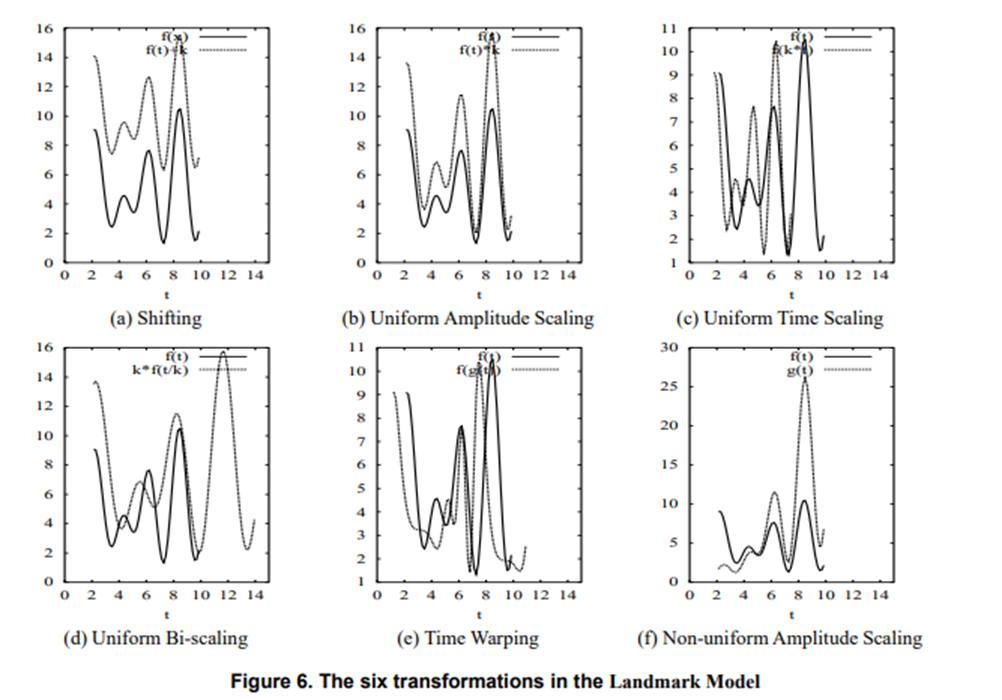
\includegraphics[scale=0.4]{figures/03-teoria/theSixTransformationsInTheLandmarkModel.png}
                \caption{Transformations in Landmark Model}
                \label{fig:scr46}
            \end{figure}
            \par
            Wybór cech charakterystycznych:
            Różne cechy są wykorzystywane do różnych zastosowań, od prostych cech (minima lokalne, maksima lokalne, punkty przełamania) do bardziej skomplikowanych
            Im więcej typów cech, tym dokładniejsze wyniki
            Punkt charakterystyczny n-tego rzędu danej krzywej jest wtedy, gdy pochodna n-tego rzędu znajduje się na tym punkcie – lokalne minima/maksima są punktami 1 rzędu, a punkty przegięcia – 2 rzędu
            Im bardziej zmienny wykres, tym mniejsze znaczenie mają punkty charakterystyczne wyższych rzędów
            \par
            Wygładzanie: Minimal Distance/Percentage Principle (MDPP) 
            Przykład MDPP(5, 5\%) – znaczy: pomiar raz na 5 dni, od 5\% wzrost lub spadek zaczyna być znaczący. Zmiany większe niż 5\% nie zostaną wygładzone
            \par 
            Obliczanie podobieństwa: Porównujemy sekwencje landmarków (a nie surowych danych)
            \begin{itemize}
                \item Pomiar niezgodności (dissimilarity measurement)
                \item Pomiar zgodności (z wykorzystaniem MDPP)
            \end{itemize}
        
        \subsection{Dynamic Time Warping}
        \label{theory:DTW}
            Metoda zakłada znalezienie optymalnego dopasowania punktów jednego przebiegu do drugiego, który ma najmniejszy koszt i spełnia wszystkie z poniższych warunków:
            Założenia przy porównywaniu dwóch sekwencji:
            \begin{itemize}
                \item Pierwsze oraz ostatnie punkty przebiegów są dopasowane do siebie
                \item Przebieg nie cofa się w czasie podczas dopasowywania
                \item Podczas dopasowania nie można wykonać zbyt długich kroków
                \item Koszt dopasowania jest sumą lokalnych odległości na tej ścieżce
            \end{itemize}
            Charakterystyka algorytmu:
            \begin{itemize}
                \item Radzi sobie ze skalowaniem czasu 
                \item Radzi sobie z przesunięciem czasu
                \item Bardziej zwraca uwagę na konkretne wartości, w porównaniu do Landmark Similarity, który głównie zwraca uwagę na punkty zwrotne
            \end{itemize}
        
        \subsection{Longest Common Subsequence}
            Jeżeli S1 i S2 to dwa ciągi, to Z jest ich wspólnym podciągiem jeżeli jest podciągiem zarówno S1, jak i S2
            Dwa ciągi są podobne jeżeli:
            (2 * Długość Z )/(Długość S1 + Długość S2) $>$= wybrana wartość progowa 
    
        \subsection{Odległość Euklidesowa}
        \label{theory:Euklides}
             Długość odcinka między punktami
            \begin{itemize}
                \item Podatny na wartości odstające
                \item Nie radzi sobie ze zeskalowanymi wykresami
                \item Wykresy muszą być tej samej długości
                \item TODO:poszukać wariacje odległości Euklidesowej
            \end{itemize}
    \section{Klasyfikacja szeregów czasowych}
        Klasyfikacja to jeden z znanych problemów, które staramy rozwiązywać się przy pomocy uczenia maszynowego. Jej celem jest przypisanie rekordów zbioru danych do odpowiedniej grupy. Klasyfikacja używa odpowiedniej funkcji mapującej zbiór cech na klasę, gdzie funkcja ta nauczona jest na zbiorze danych treningowych\cite{Classification_theory}. Przykładowe algorytmy, które rozwiązują ten problem to \textit{Support Vector Machine (SVM)}, \textit{Drzewa decyzyjne}, \textit{KNN} i wiele innych, jednak niekonieczne nadają się one do problemu szeregów czasowych.
        
        W przypadku szeregów czasowych nie mamy do czynienia z zbiorem cech dla obserwacji, lecz z pomiarami zebranymi w jakimś okresie czasu. Przykładowo pomiar temperatury w ciągu dnia. Do klasyfikacje trzeba brać pod uwagę szereg jako całość a nie pojedyncze obserwacje. Dodatkowo dany szereg może posiadać więcej niż jeden typ obserwacji, wtedy poza temperaturą, mierzymy przykładowo wilgotność i prędkość wiatru. Innym czynnikiem wpływającym na zdatność algorytmu do klasyfikacji szeregów czasowych jest jego zdolność do radzenia sobie z obserwacjami o różnej długości. Jeżeli badamy pogodę każdego dnia to szeregi będą równe (24 godziny), ale nie zawsze tak jest. Badane zjawisko może mieć nieregularną długość i wtedy każda obserwacja może mieć różną długość trwania (przykładowo zużycie zasobów podczas działania algorytmu). Biorąc pod uwage te wszystkie cechy szeregów czasowych szukaliśmy specyficznych algorytmów, które poradzą sobie z tymi wyzwaniami.
        
        \subsection{ROCKET}
            ROCKET, czyli \textbf{R}and\textbf{O}m \textbf{C}onvolutional \textbf{KE}rnel \textbf{T}ransform wykorzystuje, jak nazwa wskazuje, losowe kernele konwolucyjne do transformacji szeregów czasowych, w celu użycia wyniku tej operacji jako cech w klasyfikatorze \cite{Rocket_classifier}. Autorzy wspierali się tym, że wykorzystanie neuronowych sieci konwolucyjnych jest efektywne dla szeregów czasowych. Podali argumenty za tym, że wykorzystanie losowych kerneli konwolucyjnych oraz wykorzystanie ich wyjściowych transformacji jako cechy wejściowe dla innego klasyfikatora jest wykorzystywane w innych przypadkach z sukcesem. 
            
            Metoda ta wykorzystuje ekstremalną ilość kerneli (domyślnie używali 10.000), w których każdy generuje 2 wartości, w ten sposób każdy szereg czasowy ma wytworzoną dużą ilość cech (w przypadku domyślnych ustawień 20.000 cech). Autorzy twierdzą, że im więcej jąder tym większa dokładność klasyfikacji kosztem czasu przetwarzania. Algorytm klasyfikacji użyty po transformacjach może być dowolny, jednak autorzy polecają klasyfikatory liniowe (domyślnie użyta została \textit{regresja grzbietowa} (ang. Ridge Regression)).
            
            Główną zaletą tego podejścia poza dokładnością, która jest na równi (jak nie lepsza) z innymi nowoczesnymi metodami klasyfikacji szeregów czasowych, jest czas przetwarzania. Złożoność tego algorytmu zależy głównie od liczby kerneli, a poza tym od liczby przykładów oraz długości przebiegów czasowych. Drugim czynnikiem wpływającym na czas potrzebny na wykonanie obliczeń jest złożoność użytego klasyfikatora, więc w przypadku regresji grzbietowej zależy ona od wielkości zbioru i liczby badanych cech. Poprzez eksperymenty w pracy, autorzy pokazali, że w porównaniu z innymi algorytmami czas trwania klasyfikacji jest niższy od reszty dla tej samej liczby przykładów z utrzymaniem podobnej dokładności, co może być dobrą cechą dla naszych przyszłych eksperymentów.
            
            Podsumowując tą sekcje, metoda ROCKET zdaję się być dobrym do sprawdzenia w naszej pracy. Autorzy tekstu pisali, że implementacja w ramach której wykonywali eksperymenty była wykonana w języku Python, więc powinna być możliwość wykorzystania jej w naszych eksperymentach. Jedyne czego brakowało w artykule to wykorzystanie algorytmu dla wielowymiarowych szeregów czasowych, jednak w podsumowaniu napisali, że jest to następny krok w badań. Z względu na to jest szansa, że ten algorytm został przystosowany dla takich zbiorów danych.
        \subsection{HIVECOTE2}
            HIVECOTE, czyli Hierarchical Vote Collective of Transformation-based Ensembles to heterogeniczny meta zbiór metod klasyfikacji szeregów czasowych \cite{HiveCote}. Każdy z zawartych algorytmów dotyczy innej domeny. Można w tej metodzie znaleźć takie algorytmy jak \textit{shapelets}, słownikach bazujących na modelu ""bag-of-words"" oraz metody interwałowe. Zgodnie z badaniami autorów pracy, HIVECOTE2 średnio jest jednym z najlepszych klasyfikatorów szeregów czasowych.
            
            Konkretne modele zawarte w ramach drugiej wersji tego algorytmu to: 
            \begin{itemize}
                \item \textit{Shapelet Transform Classifier}
                \item Dostosowana wersja wcześniej wspomnianego algorytmu \textit{ROCKET} nazwana \textit{ARSENAL}
                \item \textit{Temporal Dictionary Ensemble (TDE)}
                \item \textit{Diverse Representation Canonical Interval Forest (DrCIF)}
            \end{itemize}
            Każdy z tych algorytmów jest uczony osobno i dodatkowo na potrzeby ostatecznego wyniki musi zwrócić estymacje swojej dokładności (ang. accuracy) na nieznanych im wcześniej danych. Podczas predykcji, każda z metod zwraca prawdopodobieństwo przynależności badanego szeregu do danej klasy po czym obliczana jest średnia ważona. Wagi to wcześniej obliczona dokładność poszczególnych algorytmów, która jest zmniejszona poprzez potęgowanie przez jakąś wartość (domyślnie jest to 4). Poniższy rysunek \ref{fig:hive_example} pokazuje przykładowe działanie tego algorytmu w praktyce dla problemu trzy-klasowego:
            
           \begin{figure}[H]
                \centering
                \captionsetup{justification=centering,margin=0.5cm}
                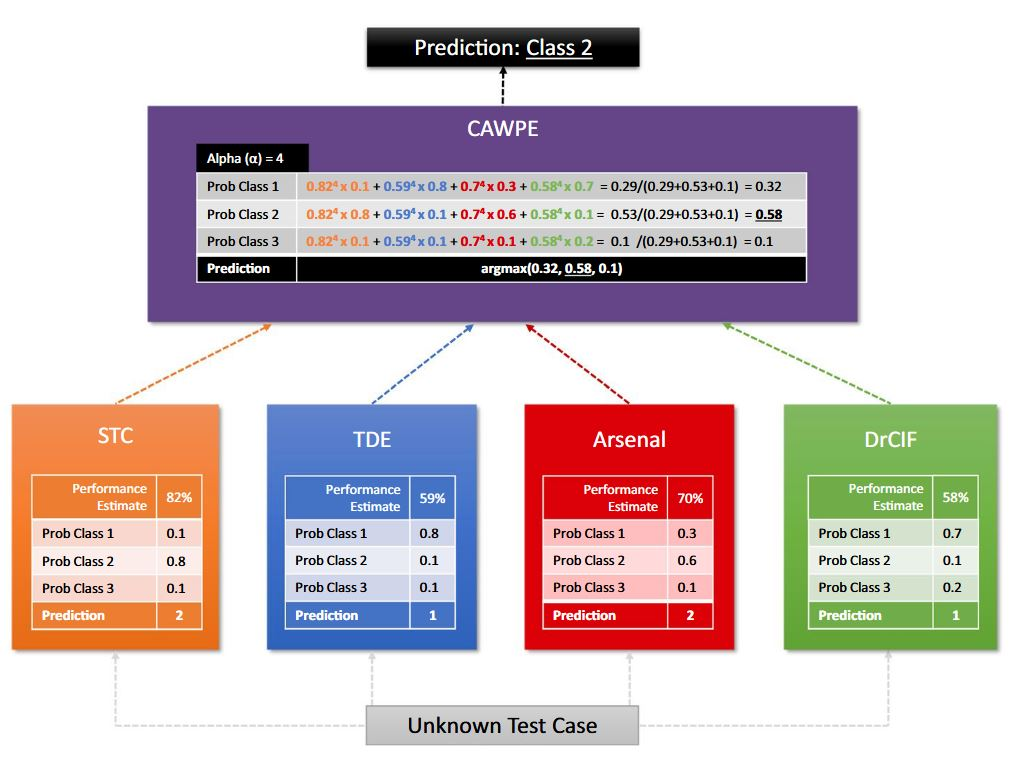
\includegraphics[scale=0.6]{figures/03-teoria/HIVE.JPG}
                \caption{Przykładowe działanie algorytmu HIVECOTE2 \cite{HiveCote}}
                \label{fig:hive_example}
            \end{figure}
            
            Jednym z zarzutów dla metody HIVECOTE2 jest jego długi czas uczenia. W porównaniu z algorytmem ROCKET jest on rzeczywiście powolny. W pracy autorzy zmieścili porównanie, gdzie ROCKET wykonuje się ponad 100 razy szybciej od algorytmu HIVECOTE2. Jednak twórcy umożliwiają ograniczenie czasu procesowania co może pozwolić nam na wygodne wykorzystanie tej metody do badań, kosztem dokładności obliczeń.
            
            Podsumowując, ten algorytm jest warty uwagi jeżeli znajdziemy jego implementacje w języku Python. Zgodnie z badaniami z opisywanej w tej sekcji pracy jest to algorytm, który powinien mieć bardzo dokładne wyniki, jeżeli pozwolimy mu wykonywać się bez ograniczeń czasowych. Jeżeli wyniki będą zadowalające dla wersji ograniczonej czasowo, eksperymenty zapewne wykonamy z tym ograniczeniem w celu oszczędzenia czasu.
        \subsection{KNN-DTW}
            Poza wyspecjalizowanymi podejściami do klasyfikacji szeregów czasowych, warto sprawdzić czy bardziej ogólne metody nadają się do badania tego problemu. Jednym z takich algorytmów jest KNN albo K-najbliższych sąsiadów (ang. K-nearest neighbor). Ta metoda przechowuje wszystkie dostępne rekordy i nadaje klasę nowemu przypadkowi na podstawie zmierzonego podobieństwa. K jest to liczba sąsiadów, których "głos"  jest wzięty pod uwagę do predykcji. Przykładowo jeżeli k = 3 to koło dookoła nowego rekordu, gdzie promieniem jest podobieństwo, będzie zawierało w sobie 3 inne przykłady. Te przykłady są wzięte do głosowania aby określić przynależność do klasy badanego przykładu \cite{Classification_theory}. 
            
            Używając tego algorytmu do przebiegów czasowych, należy wybrać odpowiednią miarę podobieństwa pasującą do tego problemu. W poprzedniej sekcji \ref{theory:podobienstwo} zbadaliśmy znane podejścia i najbardziej wyróżniającą się miarą jest \textit{Dynamic Time Warping}. Użycie tego podejścia w połączeniu z algorytmem K-NN jest sprawdzoną metodą i udowodniono, że jakość klasyfikacji w tym przypadku jest bardzo dobra, osiągająca ok. 80\% dokładności \cite{KNNDTW}. Autorzy pracy również wzięli pod uwagę inne miary podobieństwa, jednak w przypadku klasyfikacji DTW osiągnął najlepsze wyniki. Wiemy też, że istnieją implementacje tego algorytmu w języku Python co daje nam możliwość użycia go w naszej pracy.
    
    \section{Metody normalizacji danych}
        \label{section:norm}
        W pracach zajmujących się uczeniem maszynowym bardzo często występuje normalizacja danych. Przykładowo \cite{RuntimeEstimationALICE} wykorzystuje normalizacje Z-score, a w pracy \cite{BigDataParallelism} twórcy użyli skalowania Min-Max. Wykonuję się ją na etapie przygotowywania danych (ang. Preprocessing) najczęściej w celu poprawienia wyników algorytmów lub czasem nawet algorytmy wymagają znormalizowanych danych dla poprawnego działania \cite{standarization_effects}. Dzięki temu procesowi otrzymujemy wartości, które w zbiorze danych będą miały podobną skale. W tej sekcji opisane zostaną popularne metody normalizacji danych, czyli \textbf{Min-Max} oraz \textbf{Z-score}. Jedna z tych metod zostanie użyta na danych wykorzystywanych w tej pracy.
        
        \subsection{Min-Max}
            Technika normalizacji Min-Max polega na odjęciu od wartości najmniejszej wartości z dziedziny i następnie podzielenie jej przez największą wartość z tej samej dziedziny. Tą metodę można przedstawić za pomocą następującego wzoru: 
            \begin{equation}
            \label{eqn:minmax}
            A'_i = \frac{A_i-min(A)}{max(A) - min(A)}
            \end{equation}
            W ten sposób uzyskujemy przeskalowane wartości z zakresu od 0 do 1. Jest to dobra technika, jeżeli nie znamy rozkładu wartości naszych danych lub jeżeli wiemy, że nie jest to rozkład standardowy.
        
        \subsection{Z-score}
            Ten sposób normalizacji to skalowanie poprzez odjęcie od wartości średniej wszystkich wartości i następnie podzielenia przez odchylenie standardowe zbioru. Wzór prezentuje się następująco:
            \begin{equation}
            \label{eqn:minmax}
            A'_i = \frac{A_i-mean(A)}{std(A)}
            \end{equation}
            Ta technika nie jest ograniczona przez żaden predefiniowany zakres wartości. Sprawia ona że średnia jest równa 0, a odchylenie standardowe 1. Użycie tej metody jest preferowane, jeżeli znamy rozkład wartości i jest on rozkładem standardowym.

\chapter{Opis danych}

Pierwszym korkiem w celu przeprowadzenia eksperymentów było zdobycie odpowiednich danych wejściowych. Zadanie to było proste, gdyż otrzymaliśmy dostęp do zbioru danych, wytworzonego w trakcie pracy, na której bazujemy naszą tezę \textbf{ODPOWIEDNI REFERENCE}. Znaleźć je można na repozytorium w serwisie GitHub.com utworzonym przez autorów poprzedniej pracy\footnote{\url{https://github.com/pientaa/spark-udf-characteristics}}.
Dane te zostały zebrane podczas przetwarzania w środowisku Apache Spark z każdego skonfigurowanego węzła i zapisane w formacie CSV w odpowiednim folderze. W sumie otrzymaliśmy 33,600 surowych plików, gdzie każdy plik to osobny przebieg wykonywania się funkcji.Struktura tych danych prezentuje się następująco:\\ 
\noindent'$<$typ przetwarzania$>$/$<$nazwa UDF$>$/$<$konfiguracja klastra$>$/source-data/node-$<$id węzła$>$/$<$data uruchomienia$>$.csv'\\
przykładowo:
\begin{figure}[H]
    \centering
    \captionsetup{justification=centering,margin=0.5cm}
    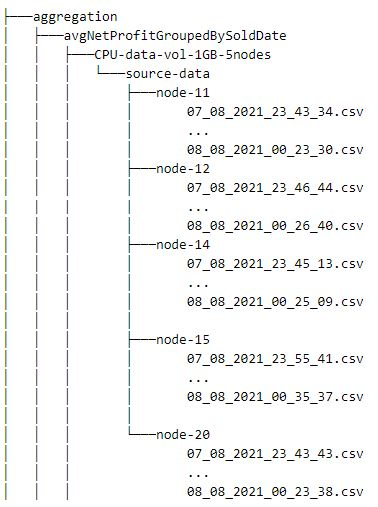
\includegraphics[scale=0.8]{figures/04-opis-danych/folder_structure.JPG}
    \caption{Struktura surowych danych}
    \label{fig:raw_file_structure}
\end{figure}
Każda funkcja została uruchomiona 25 razy per konfiguracja klastra. W każdym węźle zawarte są informacje o zużyciu procesora i pamięci RAM w trakcie wykonywania się UDF'a dla utworzonych procesów. Z tego powodu dla jednego momentu w czasie może być zaraportowanych parę procesów z ich zużyciem zasobów. Wszystko to jest zebrane w pliku CSV o następującym schemacie:
\begin{itemize}
    \item timestamp - znacznik czasowy w formacie 'rok-miesiąc-dzień godzina:minuta:sekunda.milisekunda'.
    \item PID - identyfikator procesu.
    \item CPU - procent zużycia procesora przez proces, dla zadań wielordzeniowych może przekroczyć 100\%.
    \item RAM - procent zużycia pamięci przez proces.
\end{itemize}
\section{Wstępne przetwarzanie danych}
Dane w tym stanie nie nadają się do eksperymentów, więc wpierw należało je uporządkować i zapisać w wygodnym dla nas formacie. Wpierw konieczne było pozbycie się podziału na procesy. Dla nas najbardziej interesujący jest sumaryczny przebieg zużycia zasobów na poziomie całej funkcji, a niż poszczególnych procesów. W tym celu wykorzystaliśmy bibliotekę \textbf{Pandas} często wykorzystywaną w przetwarzaniu danych. Wpisy zostały pogrupowane po znacznikach czasowych i procenty zużycia zasobów (kolumny CPU oraz RAM) zsumowane w ramach jednej grupy oraz usunięte identyfikatory procesów, gdyż nie są one nam do niczego potrzebne. Dodatkowo kolumna 'timestamp' zastąpiona jest kolumną 'epoch', która opisuje liczbę sekund (z dokładnością do 16 miejsc po przecinku) która minęła od uruchomienia funkcji.

Otrzymane zbiory zostały zapisane w takiej samej strukturze, ale w osobnym nad-folderze 'Prepared'.

W dalszym ciągu pozostaje kwestia zawartości poszczególnych folderów węzłów. Dla każdego uruchomienia funkcji posiadamy przebiegi o zużyciu w każdym węźle, zamiast ogólnie dla UDF'a. Dodatkowo bazując na pracy pilotażowej, wiemy że nie każdy więcej aktywnie brał udział w obliczeniach. Jeden z węzłów był zawsze używany jako master, którego zadaniem było zarządzanie wykonywaniem się zadań na klastrach pracujących (workers). Jeżeli master nie nadał zadania każdemu z klastrów pracujących, to taki węzeł nic nie robił poza wysyłaniem okazyjnie informacji o stanie (tzn. czy jest wciąż aktywny). Z tego powodu następnym krokiem było odfiltrowanie wszystkich węzłów bezczynnych oraz mastera i zachowanie jednie tych, które wykonywały jakieś obliczenia.

Założyliśmy, że master, ze względu na to, że nie wykonuje pracy na danych nie powinien wykorzystywać zbyt dużo pamięci RAM. I faktycznie dla każdego eksperymentu można było znaleźć jeden węzeł, którego średnie zużycie RAM było wyraźnie mniejsze. Eksperymentując ustaliliśmy próg 2\% - odrzuciliśmy wszystkie węzły, dla których średnie zużycie RAM było poniżej tego progu.

Następnym krokiem było znalezienie i wykluczenie węzłów niepracujących. Jako, że takie węzły wysyłały tylko okazyjne informacje o tym, że wciąż są aktywne to różnice między zużyciem CPU dla nich i dla węzłów pracujących również były wyraźnie widoczne. Dokładnie to było widać zwłaszcza w kilku początkowych pomiarach, które dla węzłów pracujących charakteryzowały się wysokim zużyciem CPU, co było dokładnie opisane i wytłumaczone w pracy pilotażowej. Z tego względu odrzuciliśmy węzły, których początkowe pomiary były niskie.

Ostatecznie chcieliśmy również uzyskać jak najmniej plików wejściowych, aby ułatwić dalsze przetwarzanie danych. Inspirując się przykładowym zbiorem danych wykorzystywanym do uczenia maszynowego na danych typu Time Series, utworzyliśmy pojedyncze pliki CSV per typ funkcji UDF o następującym schemacie:
\begin{itemize}
    \item snapshot - identyfikator pojedynczego przebiegu czasowego.
    \item label - opis typu funkcji, np 'aggregation'.
    \item udf - nazwa funkcji z którego pochodzi danych przebieg czasowy.
    \item epoch - liczba sekund, która minęła od uruchomienia się funkcji z dokładnością do 16 miejsc po przecinku.
    \item CPU - procent zużycia procesora przez proces, dla zadań wielordzeniowych może przekroczyć 100\%.
    \item RAM - procent zużycia pamięci przez proces.
\end{itemize}
Poniżej znajduje się przykładowe parę wierszy z tak utworzonego pliku dla funkcji typu 'aggregation':
\begin{table}[H]
\center{
 \begin{tabular}{|c|c|c|c|c|c|} 
 \hline
snapshot & label & udf & epoch & CPU & RAM \\
\hline
0 & aggregation & avgNetProfitGroupedBySoldDate & 0.0 & 206.7 & 4.8 \\
\hline
0 & aggregation & avgNetProfitGroupedBySoldDate & 0.1562700271606445 & 220.0 & 5.0 \\
\hline
0 & aggregation & avgNetProfitGroupedBySoldDate & 0.3140101432800293 & 133.3 & 5.19 \\
\hline
0 & aggregation & avgNetProfitGroupedBySoldDate & 0.4715931415557861 & 146.7 & 5.3 \\
\hline
0 & aggregation & avgNetProfitGroupedBySoldDate & 0.6280381679534912 & 126.7 & 5.4 \\
\hline
0 & aggregation & avgNetProfitGroupedBySoldDate & 0.7846581935882568 & 160.0 & 5.5 \\
\hline
\end{tabular}
}
\caption{Początek pliku joined\_aggregation.csv}
\end{table}

Zebrane tak dane mogą zostać użyte w dalszym przetwarzaniu. W zbiorze możemy wyróżnić pięć typów funkcji zależnie od rodzaju przetwarzania:
\begin{itemize}
    \item aggregation
    \item filtration
    \item filtration-aggregation
    \item filtration-aggregation-join
    \item filtration-join
\end{itemize}
Kolumna 'label' zawiera jedną z tych wartości, poniżej w celu przedstawienia przykładowych przebiegów czasowych narysowane są wykresy dla każdego z typów z podziałem na RAM i CPU.

\begin{figure}[H]
  \centering
  \subfloat[CPU]{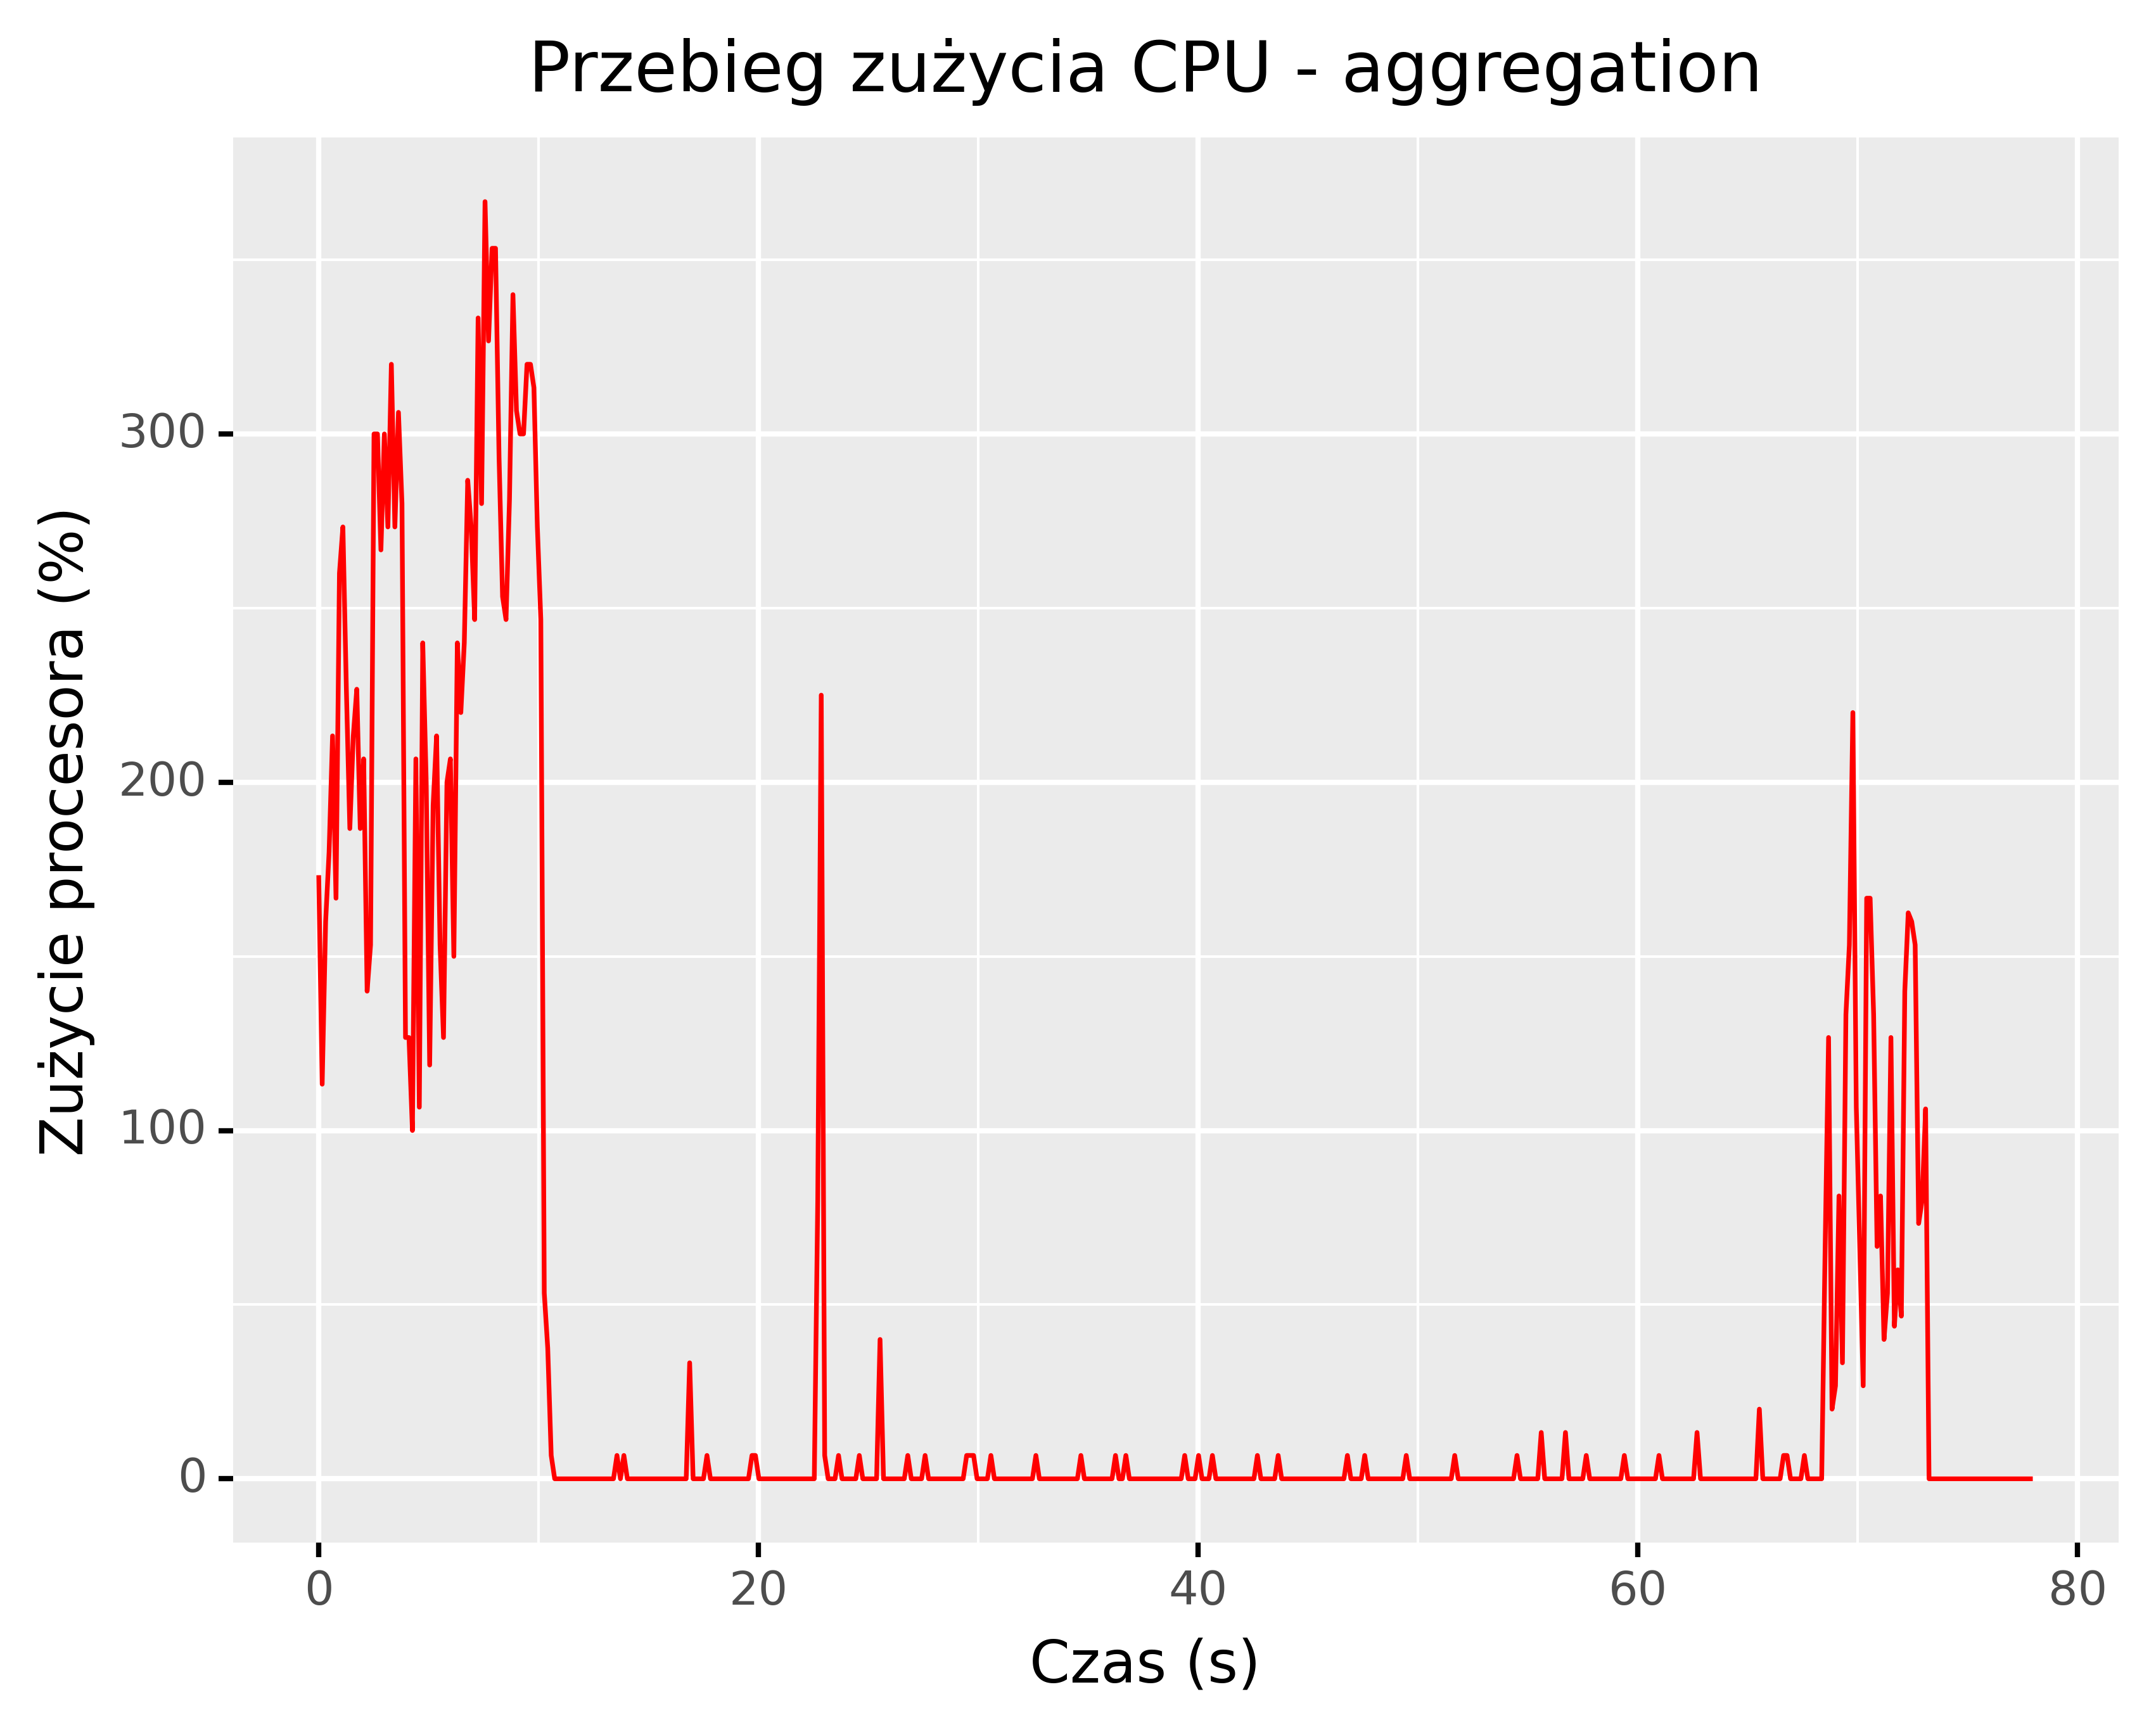
\includegraphics[width=0.5\textwidth]{figures/04-opis-danych/aggregation_example_cpu_snapshot_1.png}\label{aggregation_example:f1}}
  \hfill
  \subfloat[RAM]{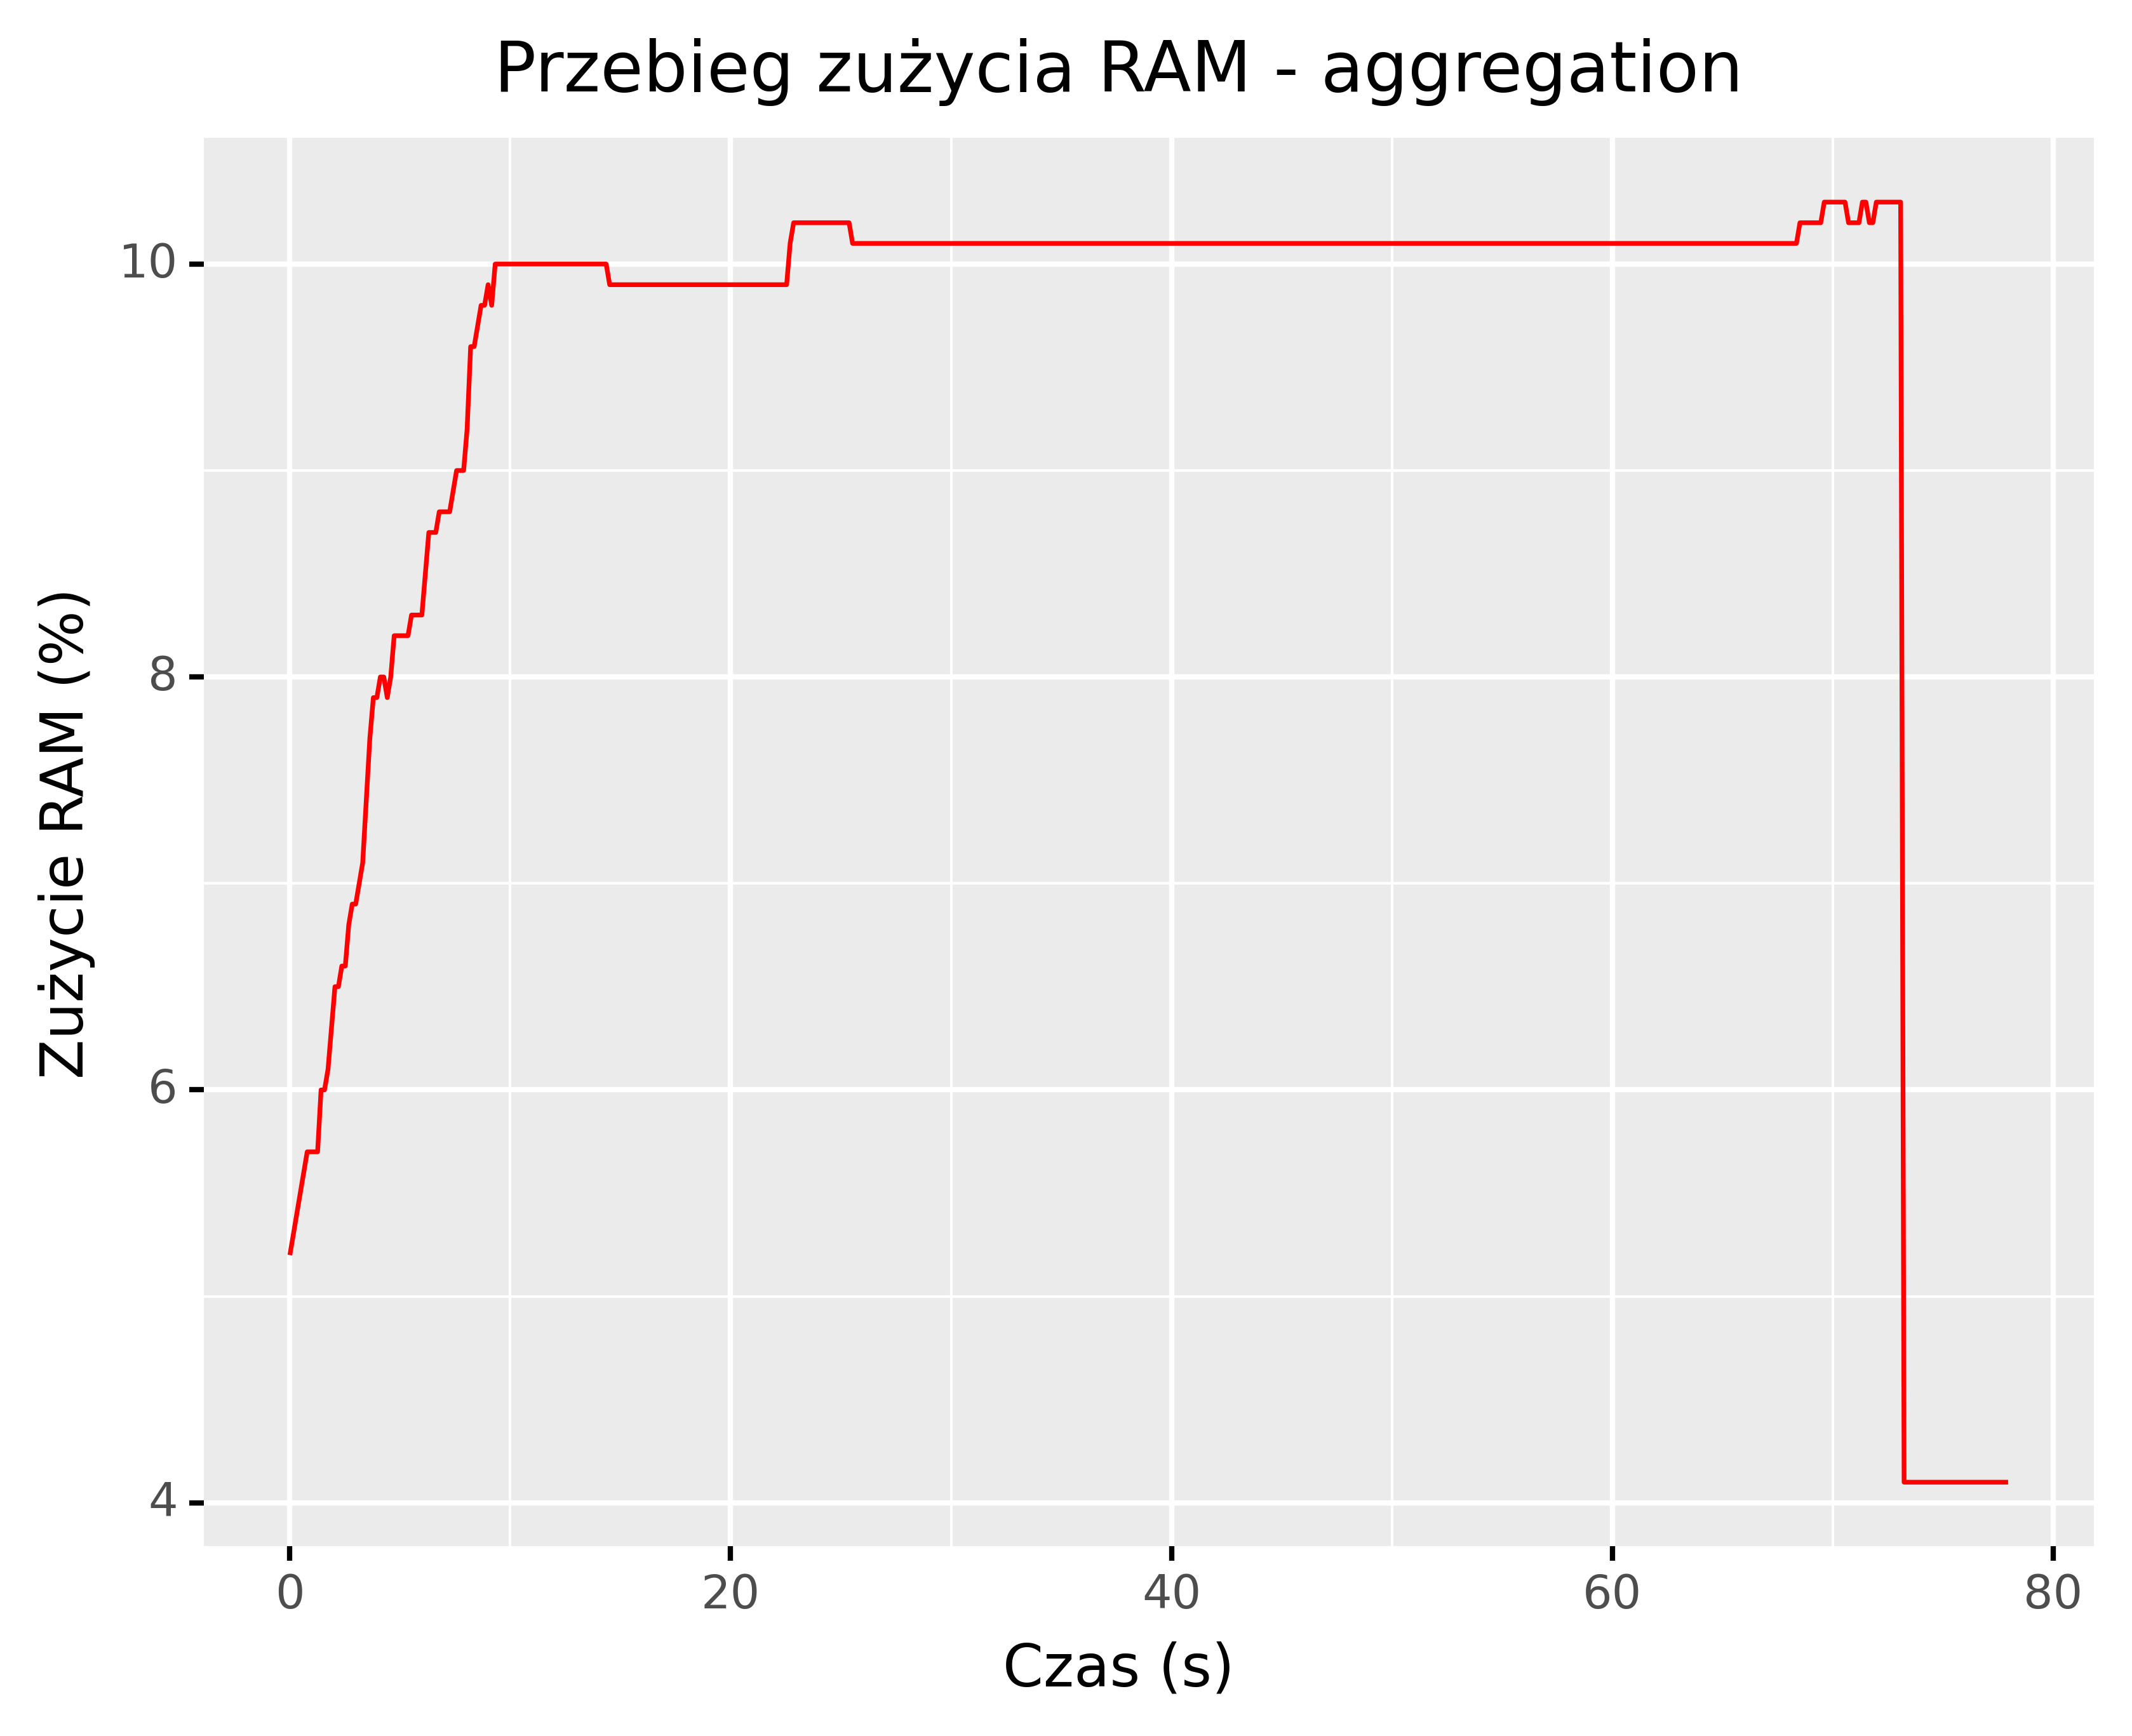
\includegraphics[width=0.5\textwidth]{figures/04-opis-danych/aggregation_example_ram_snapshot_1.png}\label{aggregation_example:f2}}
  \caption{Przykładowy przebieg zużycia zasobów dla agregacji (snapshot = 1)}
  \label{aggregation_example}
\end{figure}

\begin{figure}[H]
  \centering
  \subfloat[CPU]{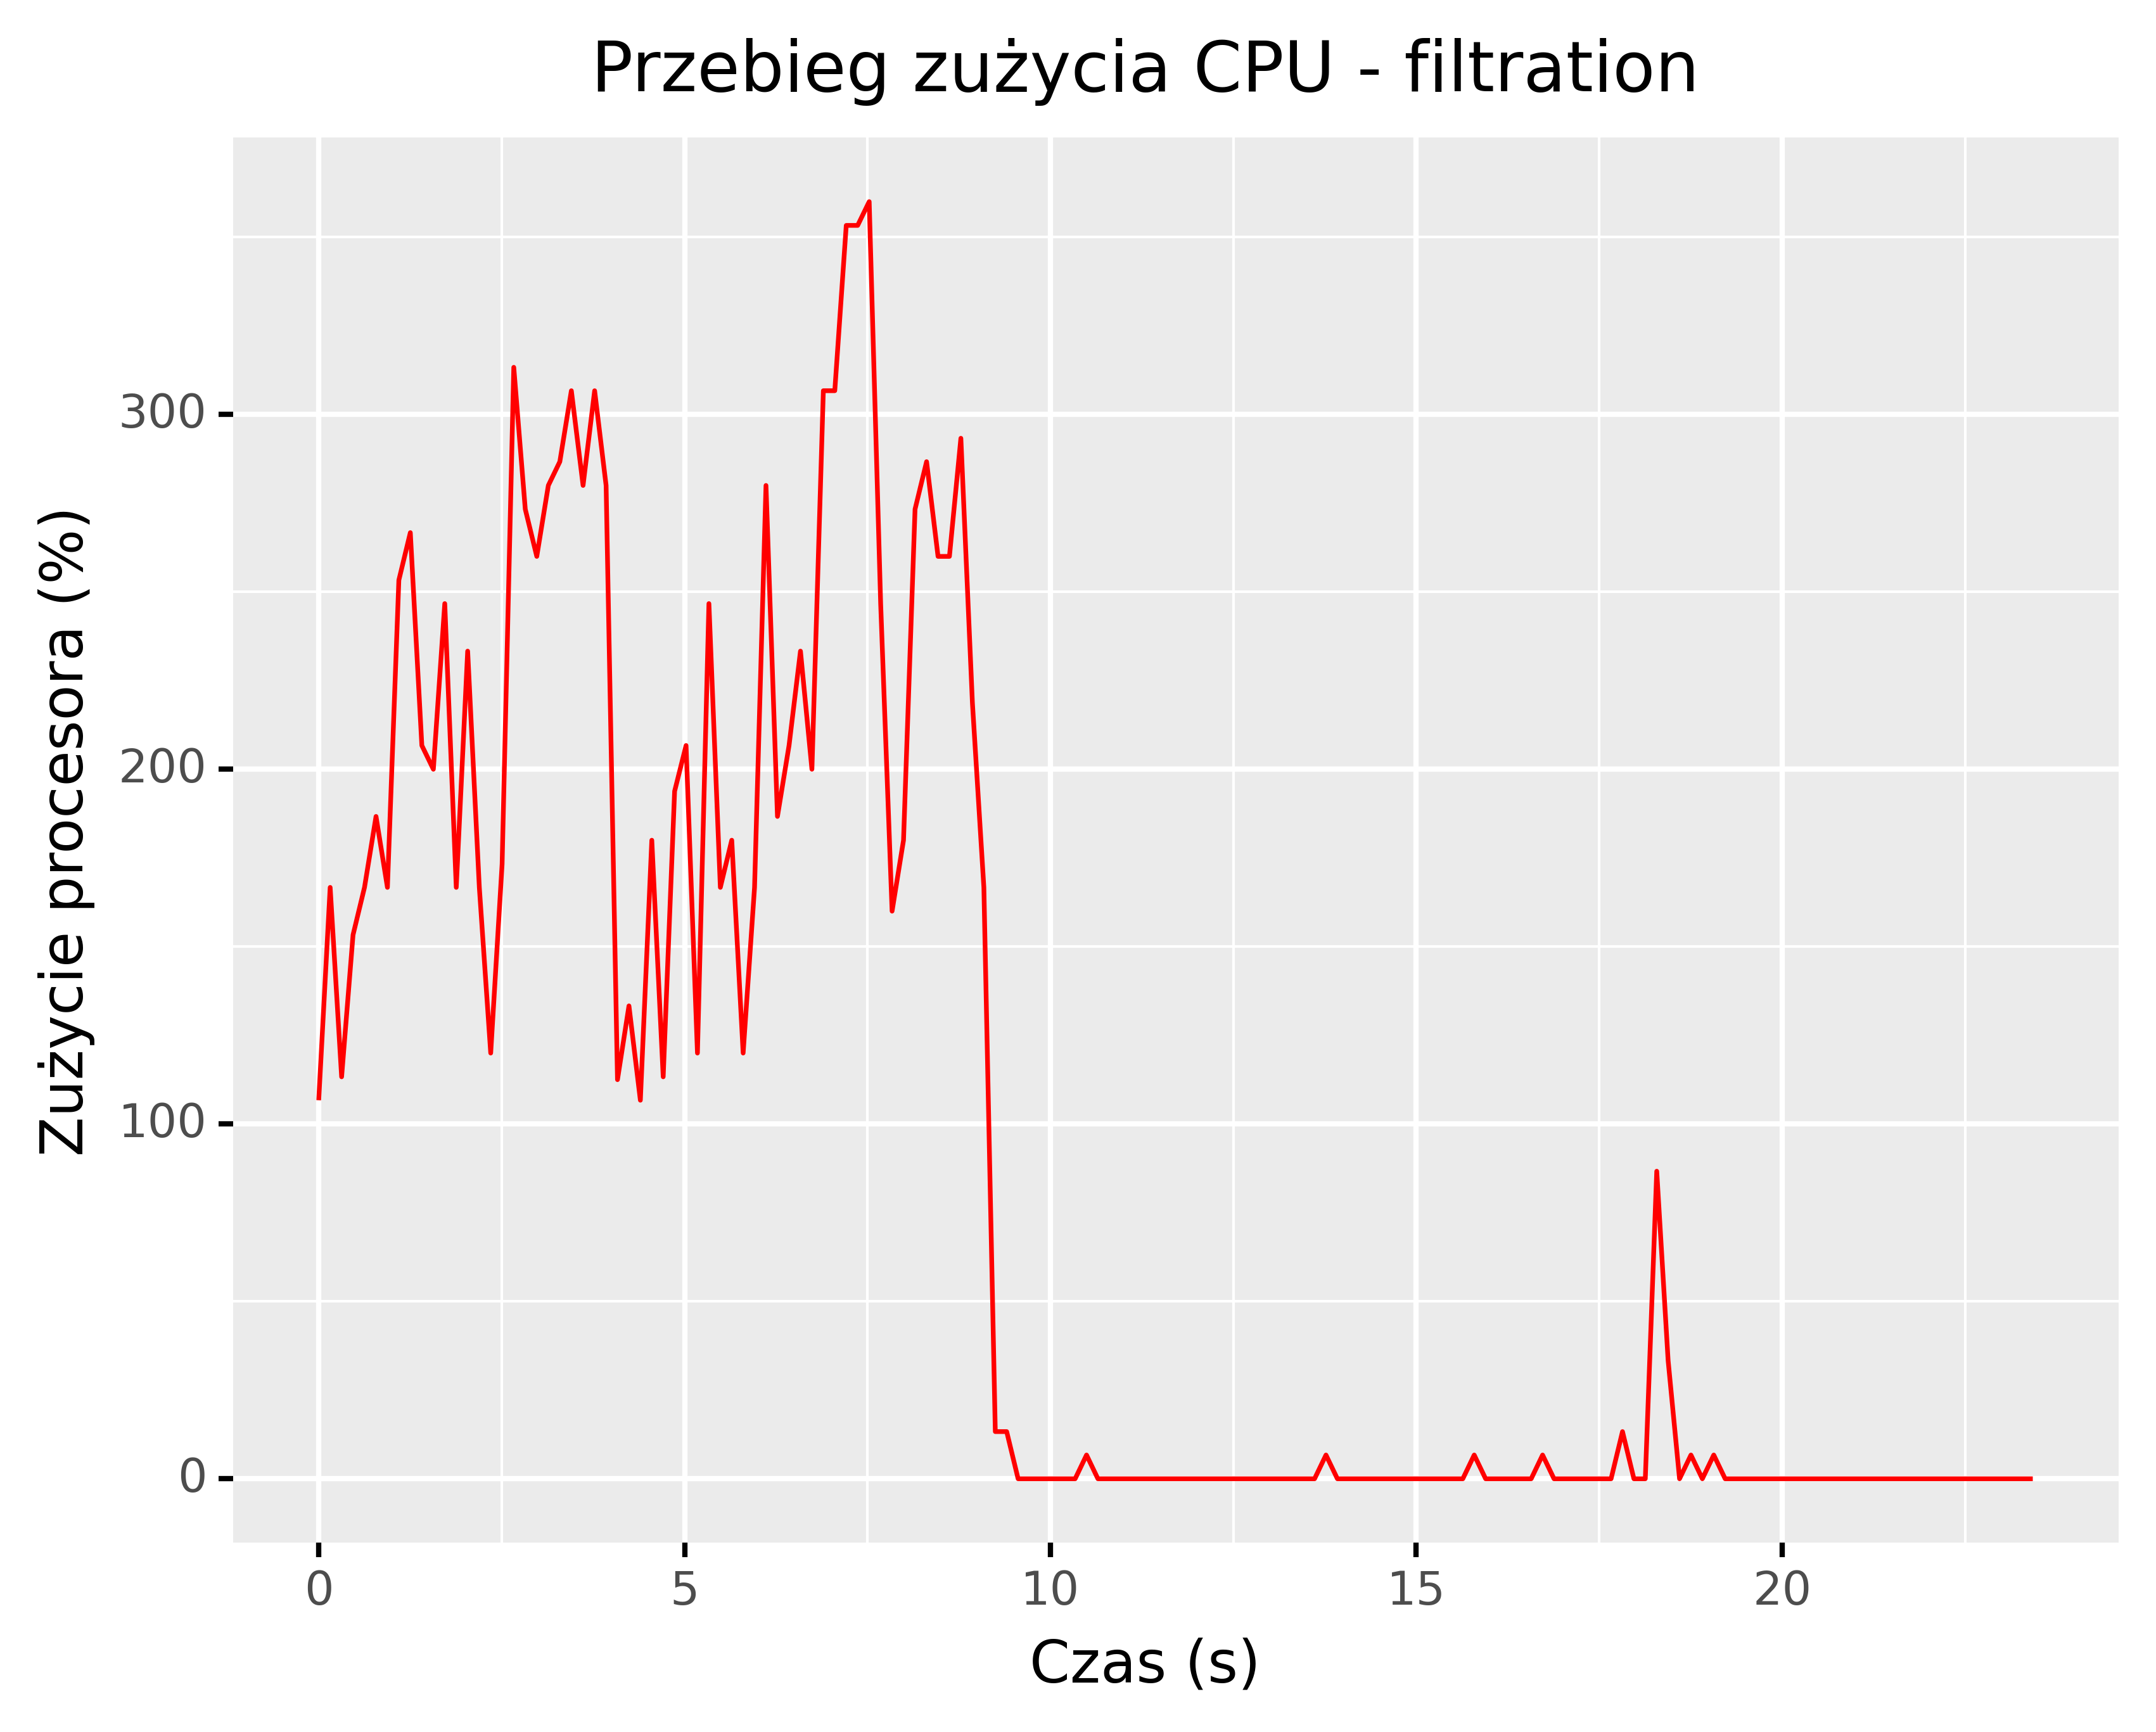
\includegraphics[width=0.5\textwidth]{figures/04-opis-danych/filtration_example_cpu_snapshot_1.png}\label{filtration:f1}}
  \hfill
  \subfloat[RAM]{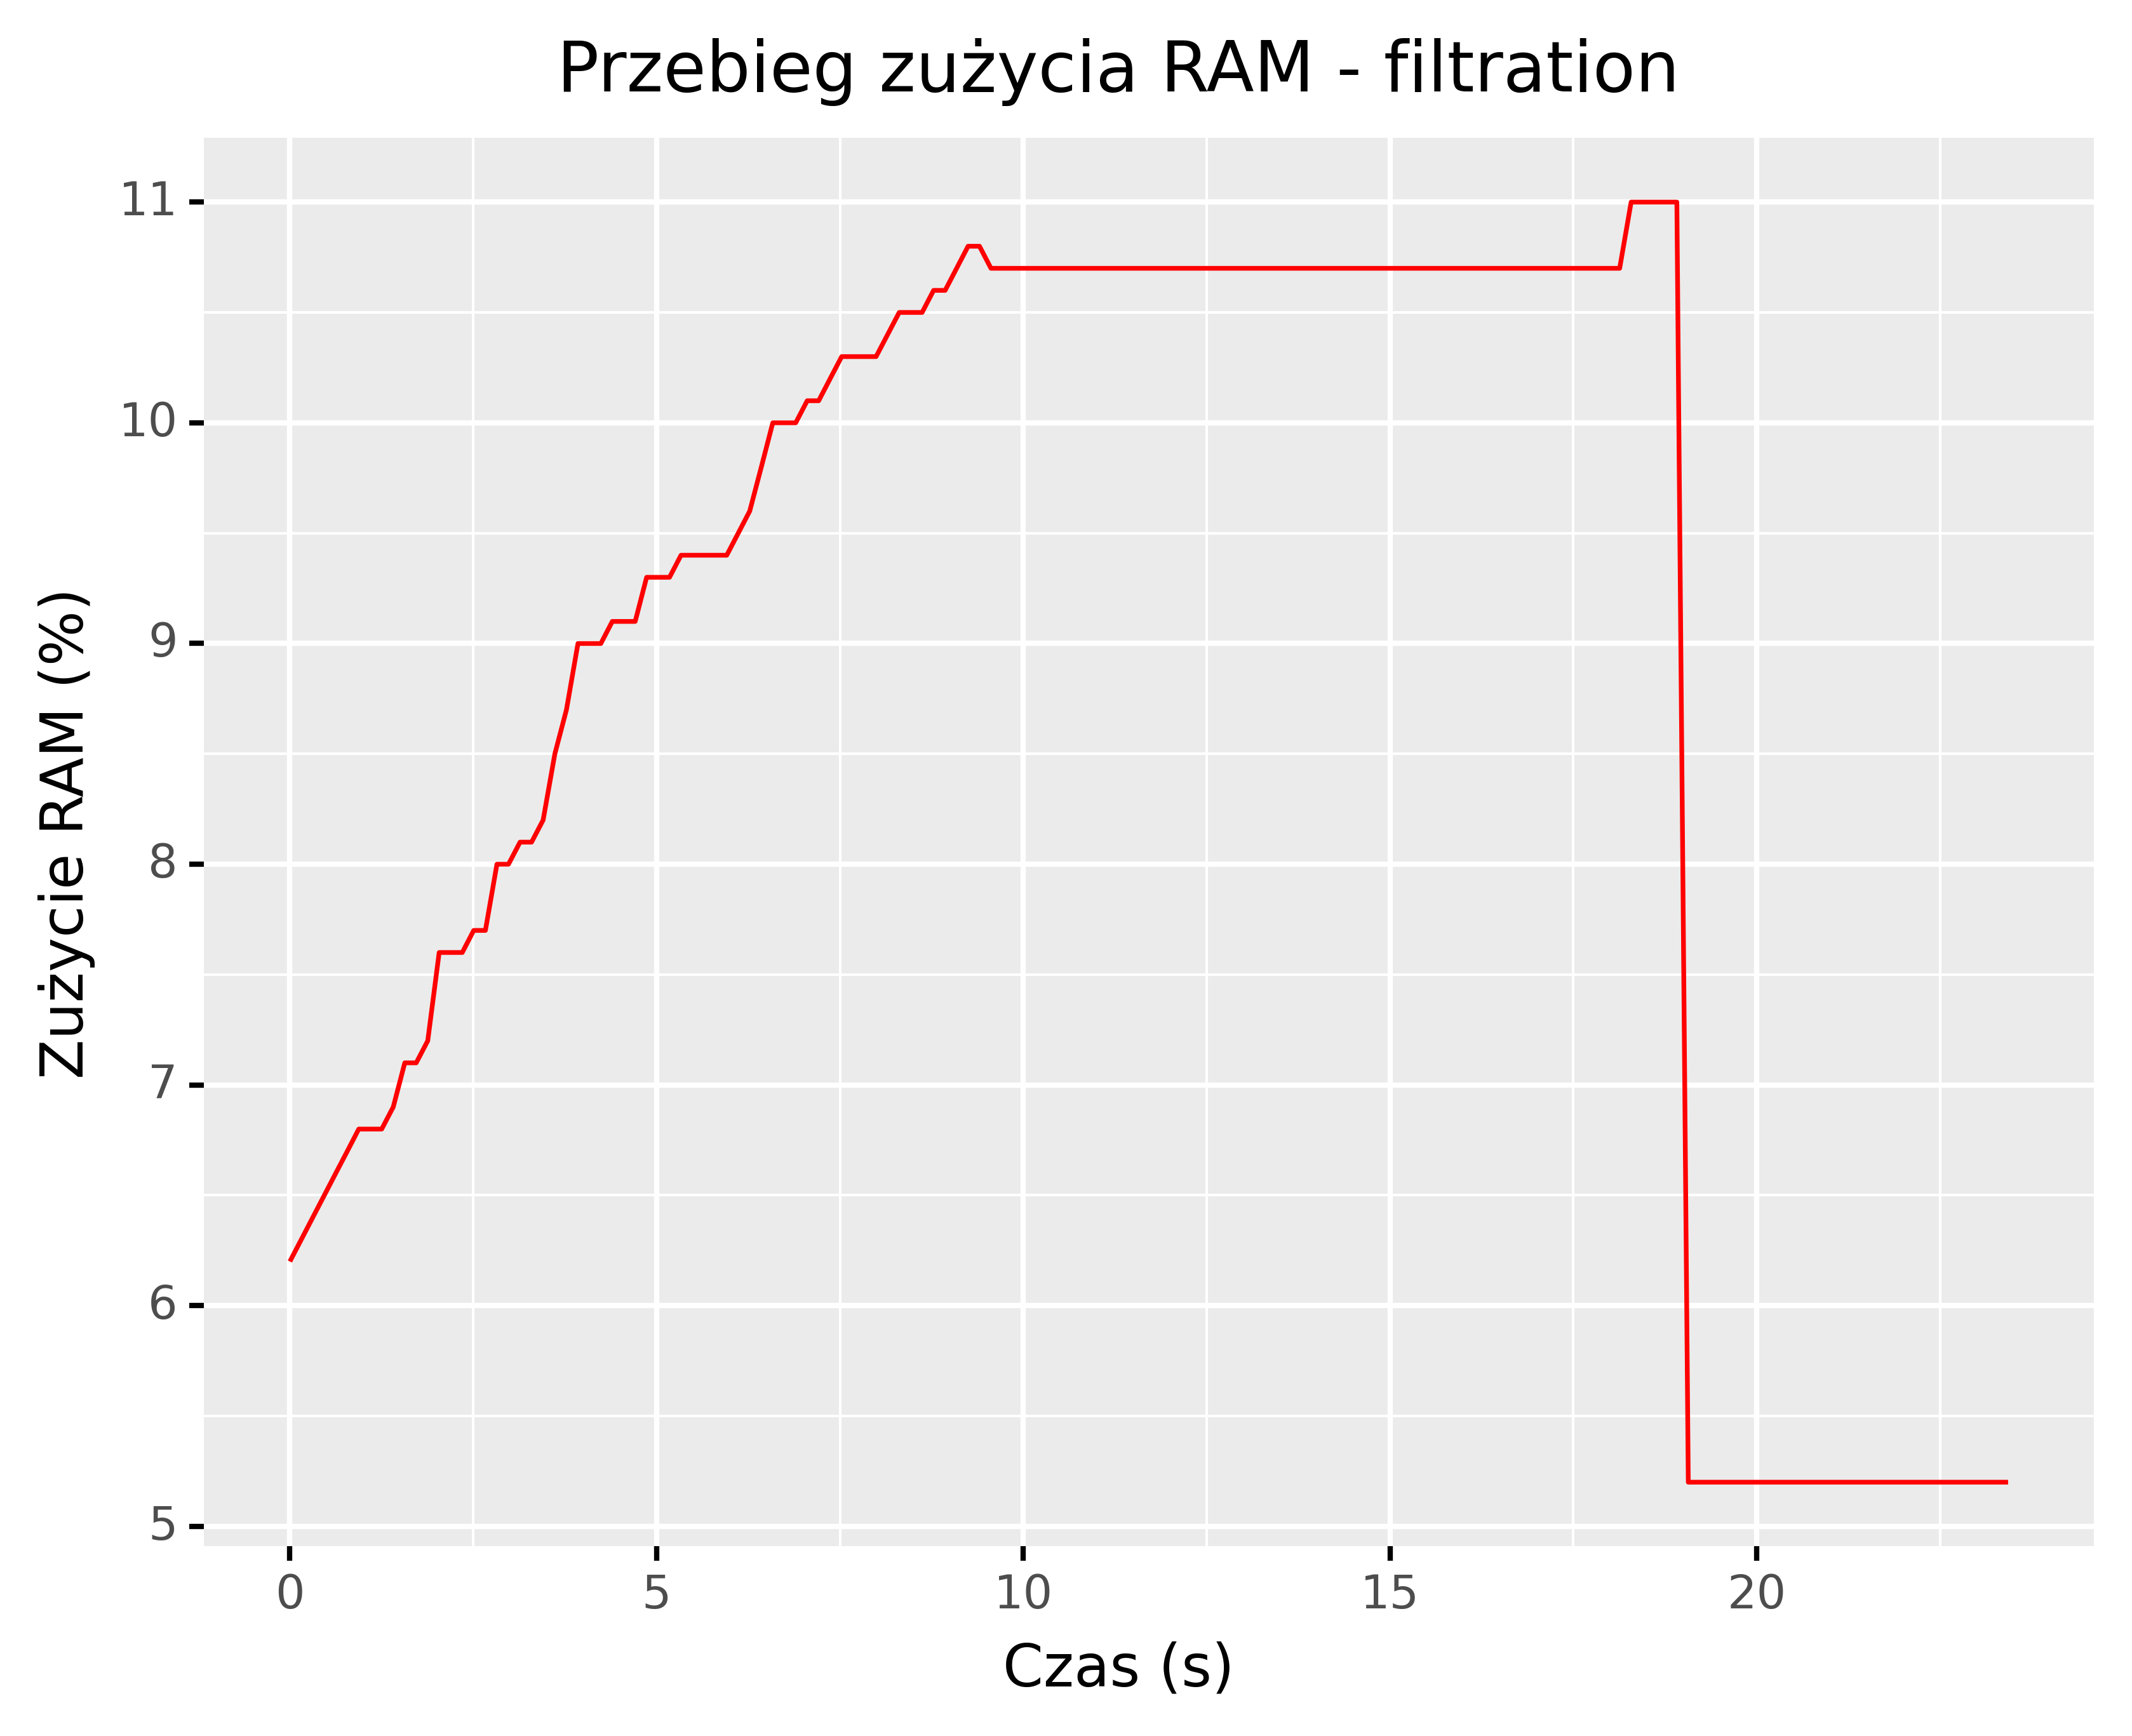
\includegraphics[width=0.5\textwidth]{figures/04-opis-danych/filtration_example_ram_snapshot_1.png}\label{filtration:f2}}
  \caption{Przykładowy przebieg zużycia zasobów dla filtracji (snapshot = 1)}
  \label{filtration_example}
\end{figure}

\begin{figure}[H]
  \centering
  \subfloat[CPU]{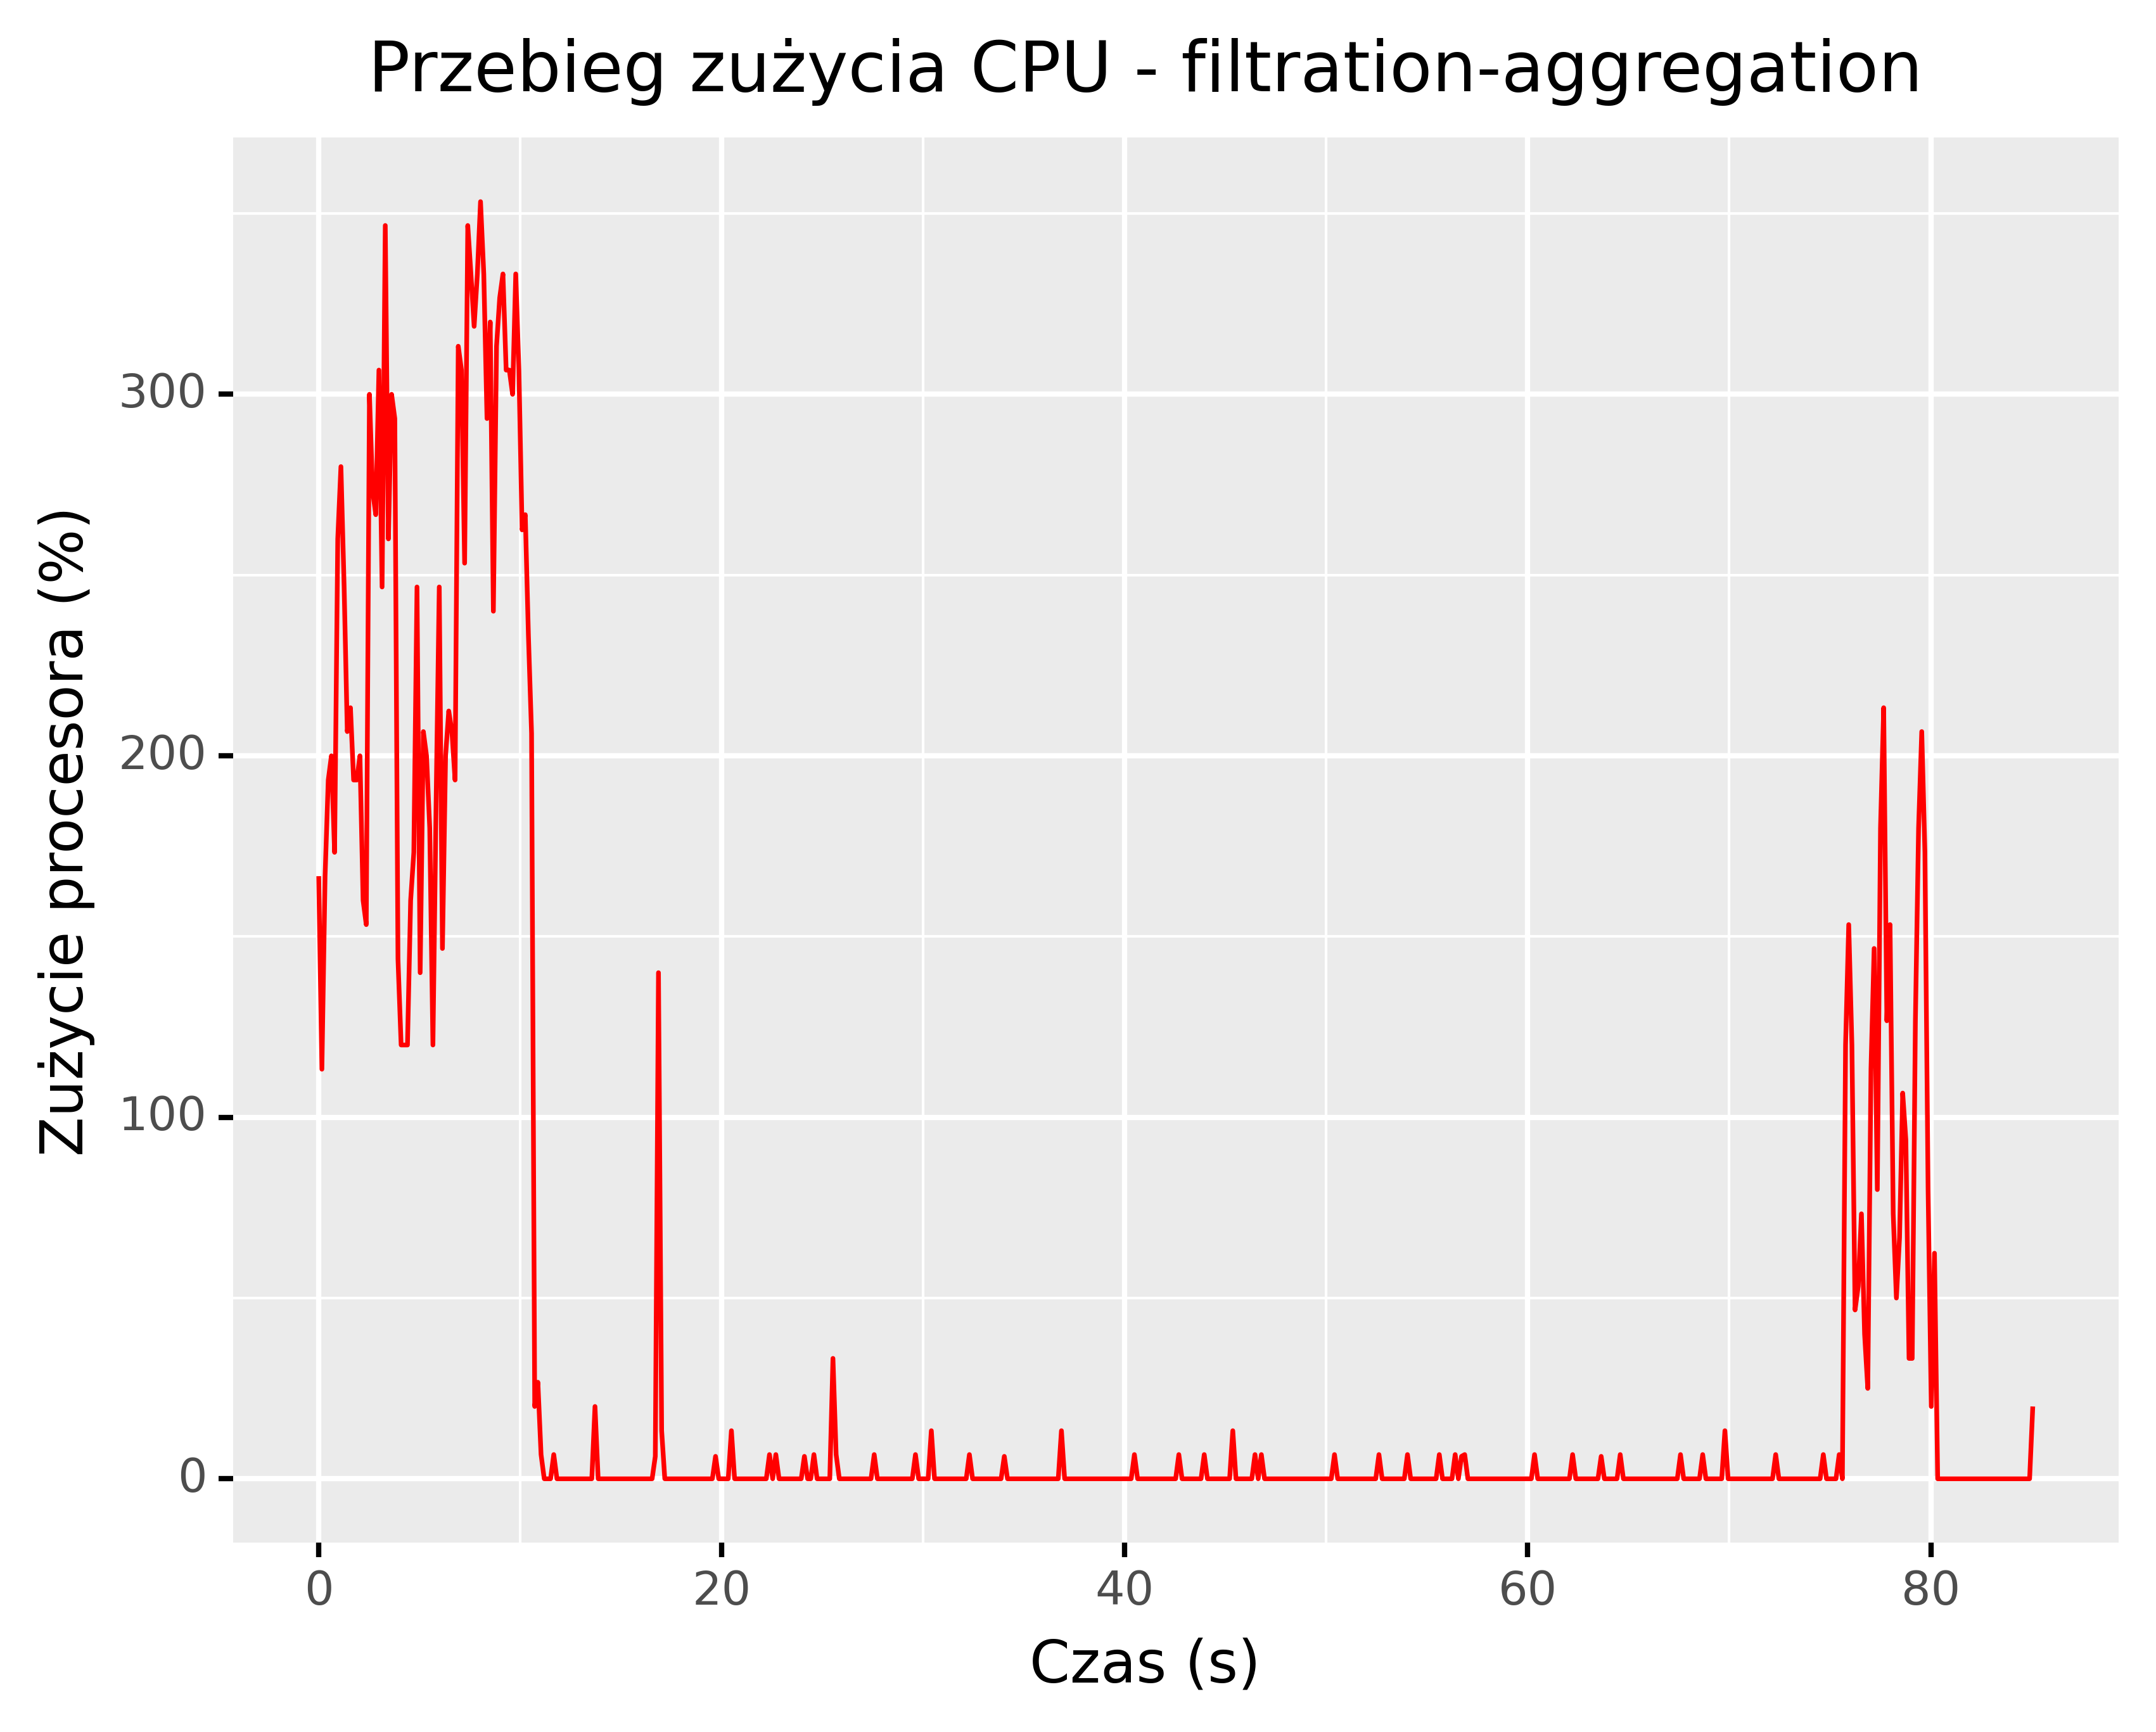
\includegraphics[width=0.5\textwidth]{figures/04-opis-danych/filtration-aggregation_example_cpu_snapshot_1.png}\label{filtration-aggregation:f1}}
  \hfill
  \subfloat[RAM]{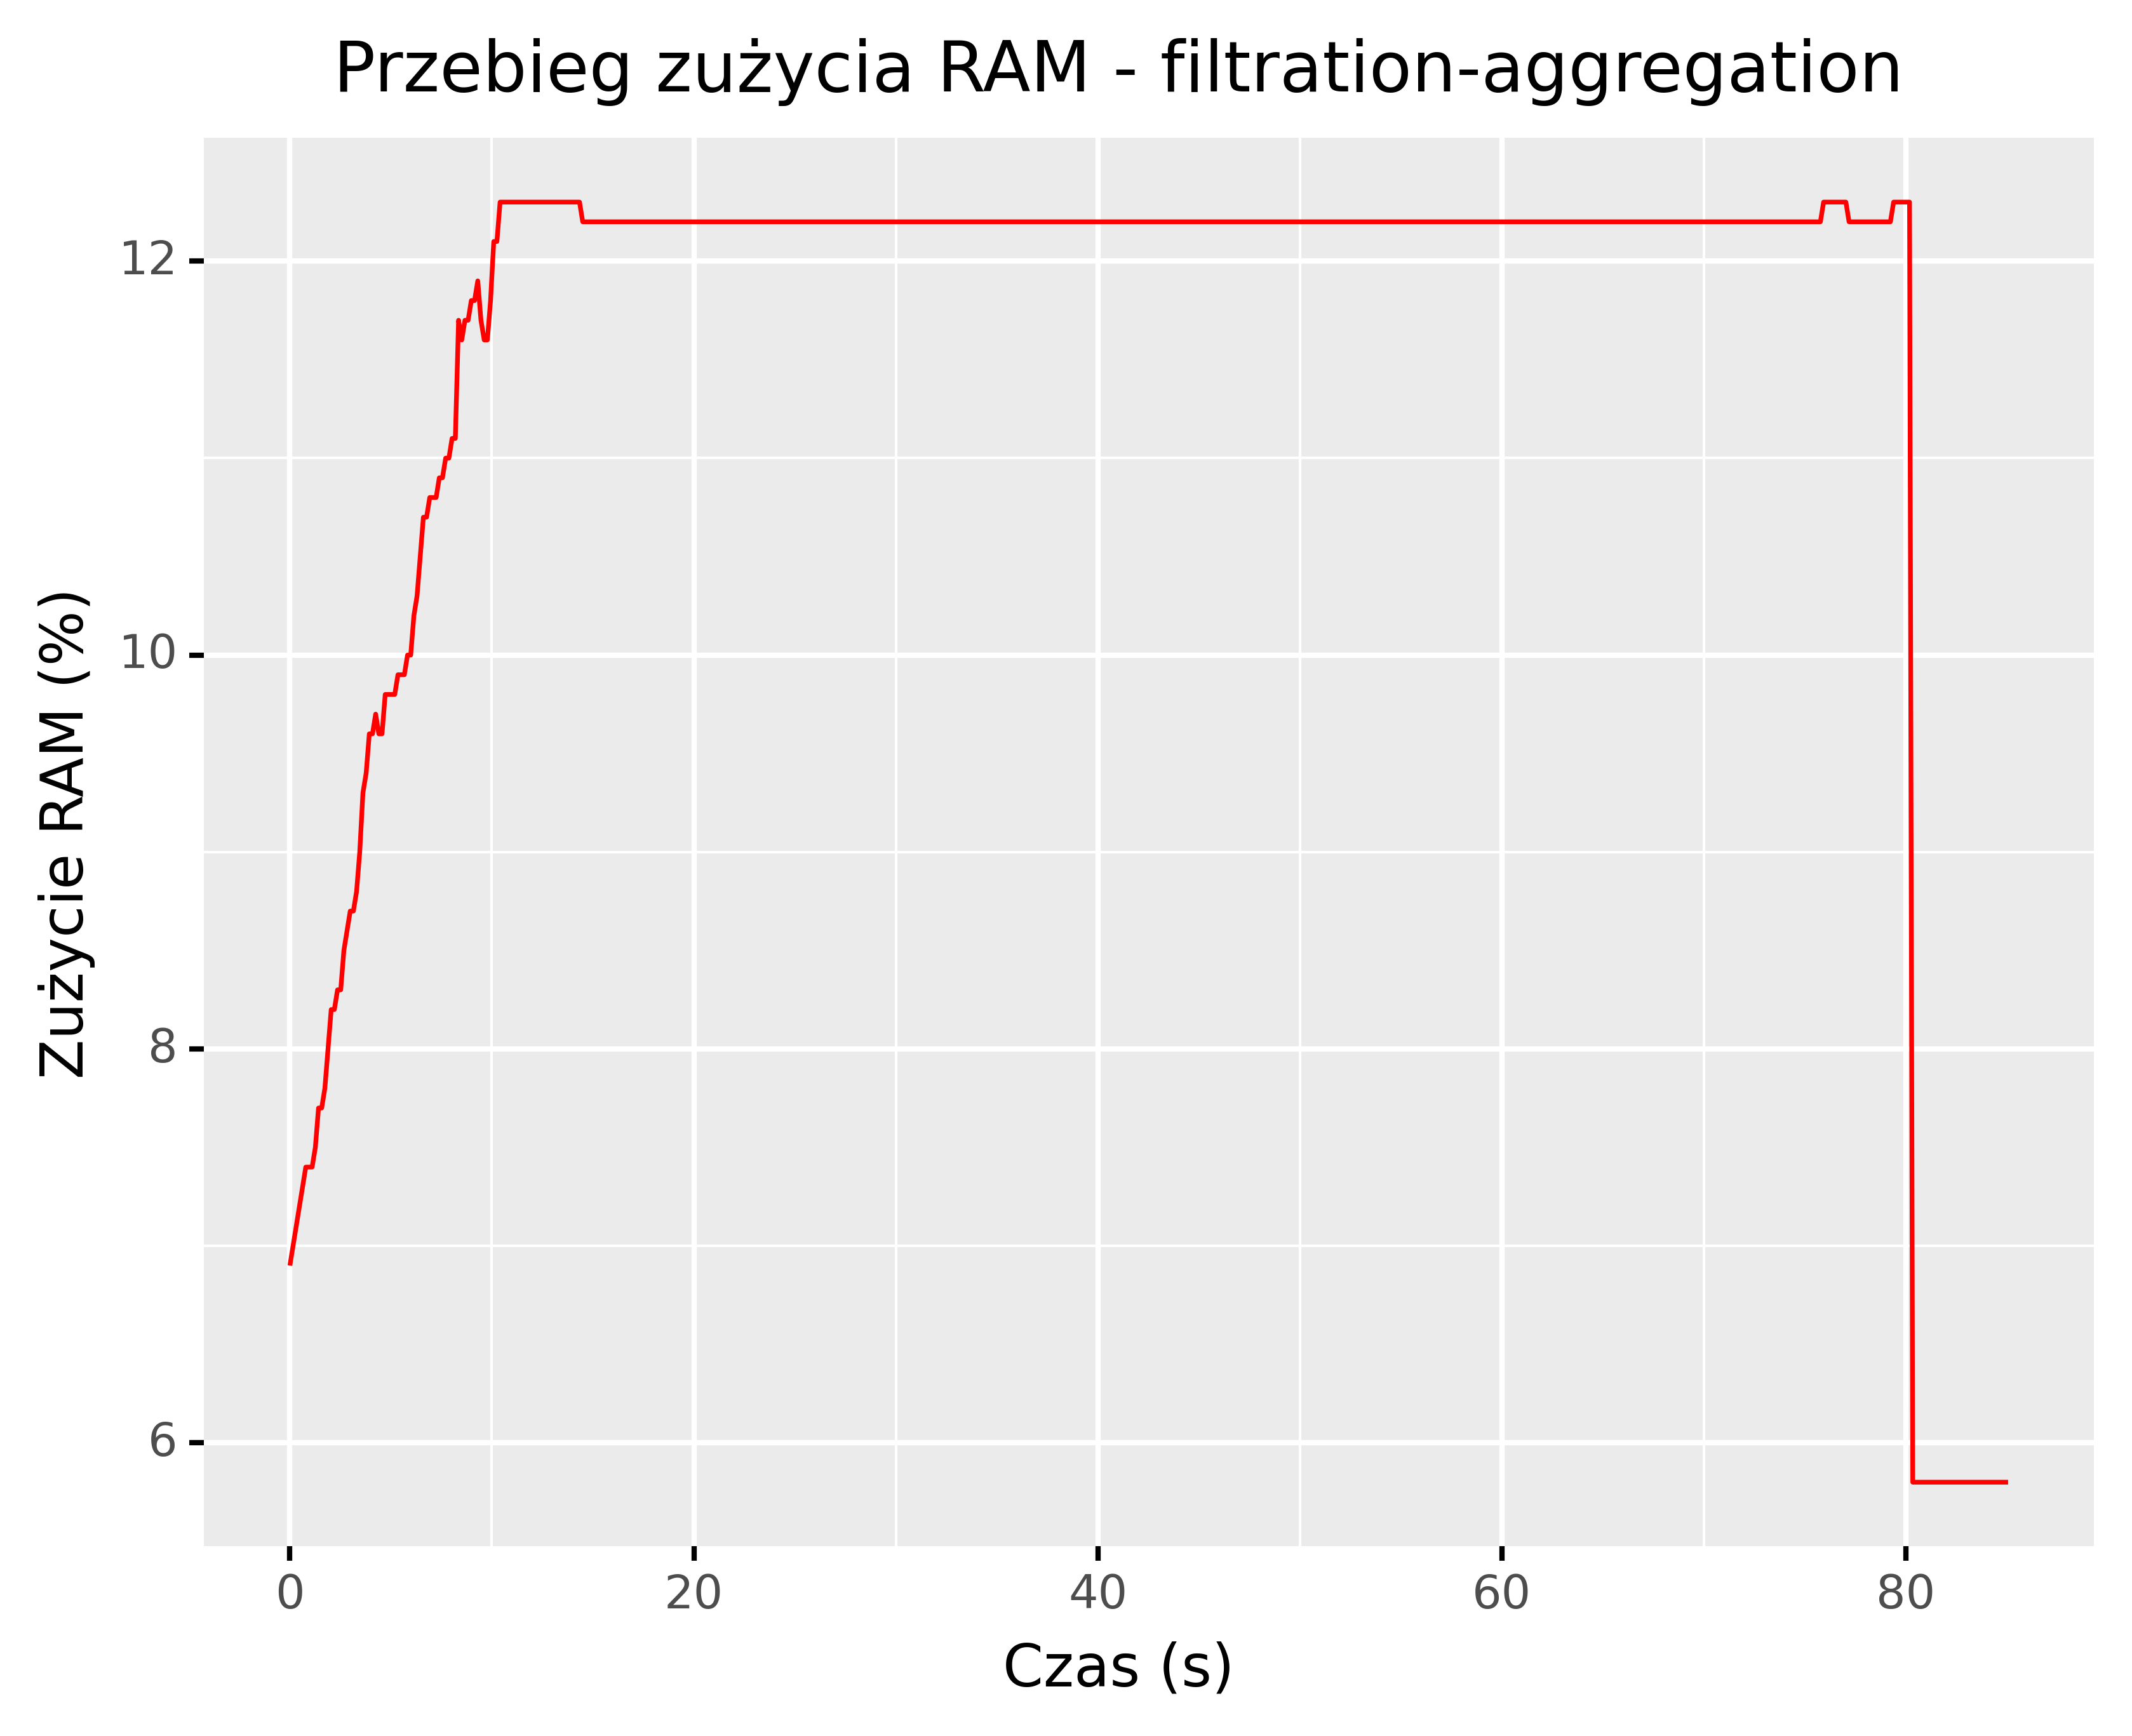
\includegraphics[width=0.5\textwidth]{figures/04-opis-danych/filtration-aggregation_example_ram_snapshot_1.png}\label{filtration-aggregation:f2}}
  \caption{Przykładowy przebieg zużycia zasobów dla filtracjo-agregacji (snapshot = 1)}
  \label{filtration-aggregation_example}
\end{figure}

\begin{figure}[H]
  \centering
  \subfloat[CPU]{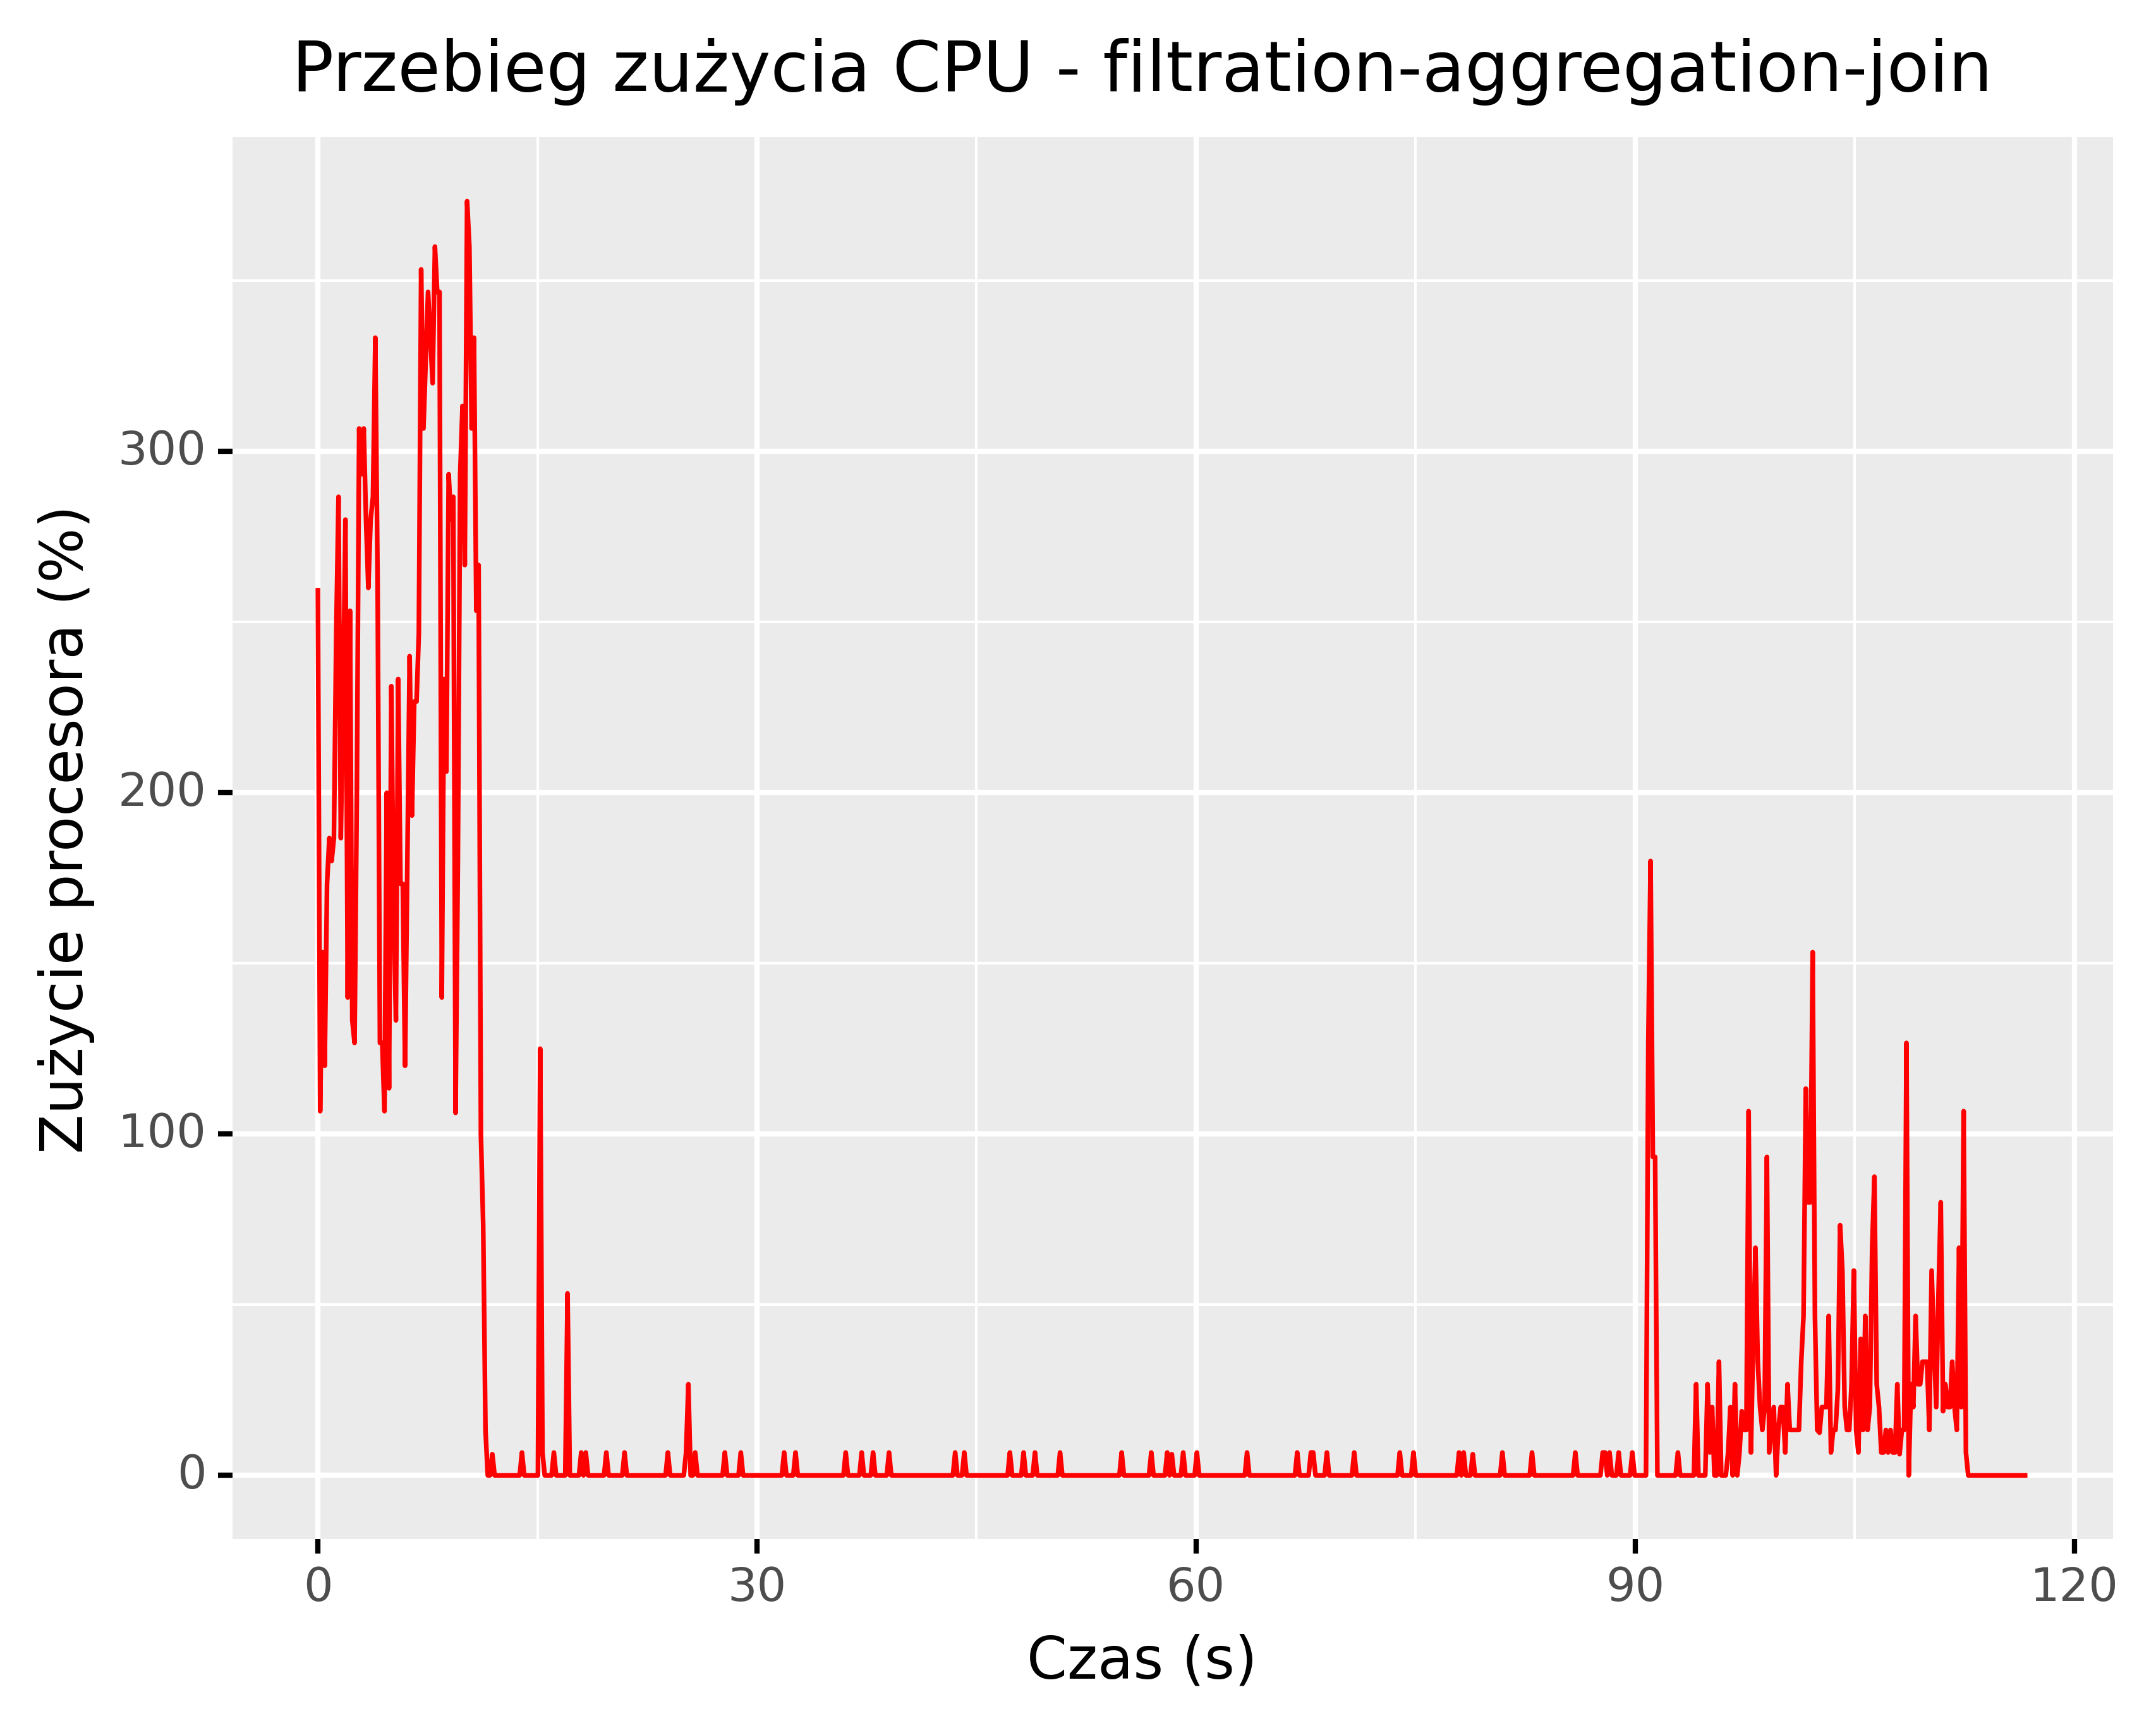
\includegraphics[width=0.5\textwidth]{figures/04-opis-danych/filtration-aggregation-join_example_cpu_snapshot_1.png}\label{filtration-aggregation-join:f1}}
  \hfill
  \subfloat[RAM]{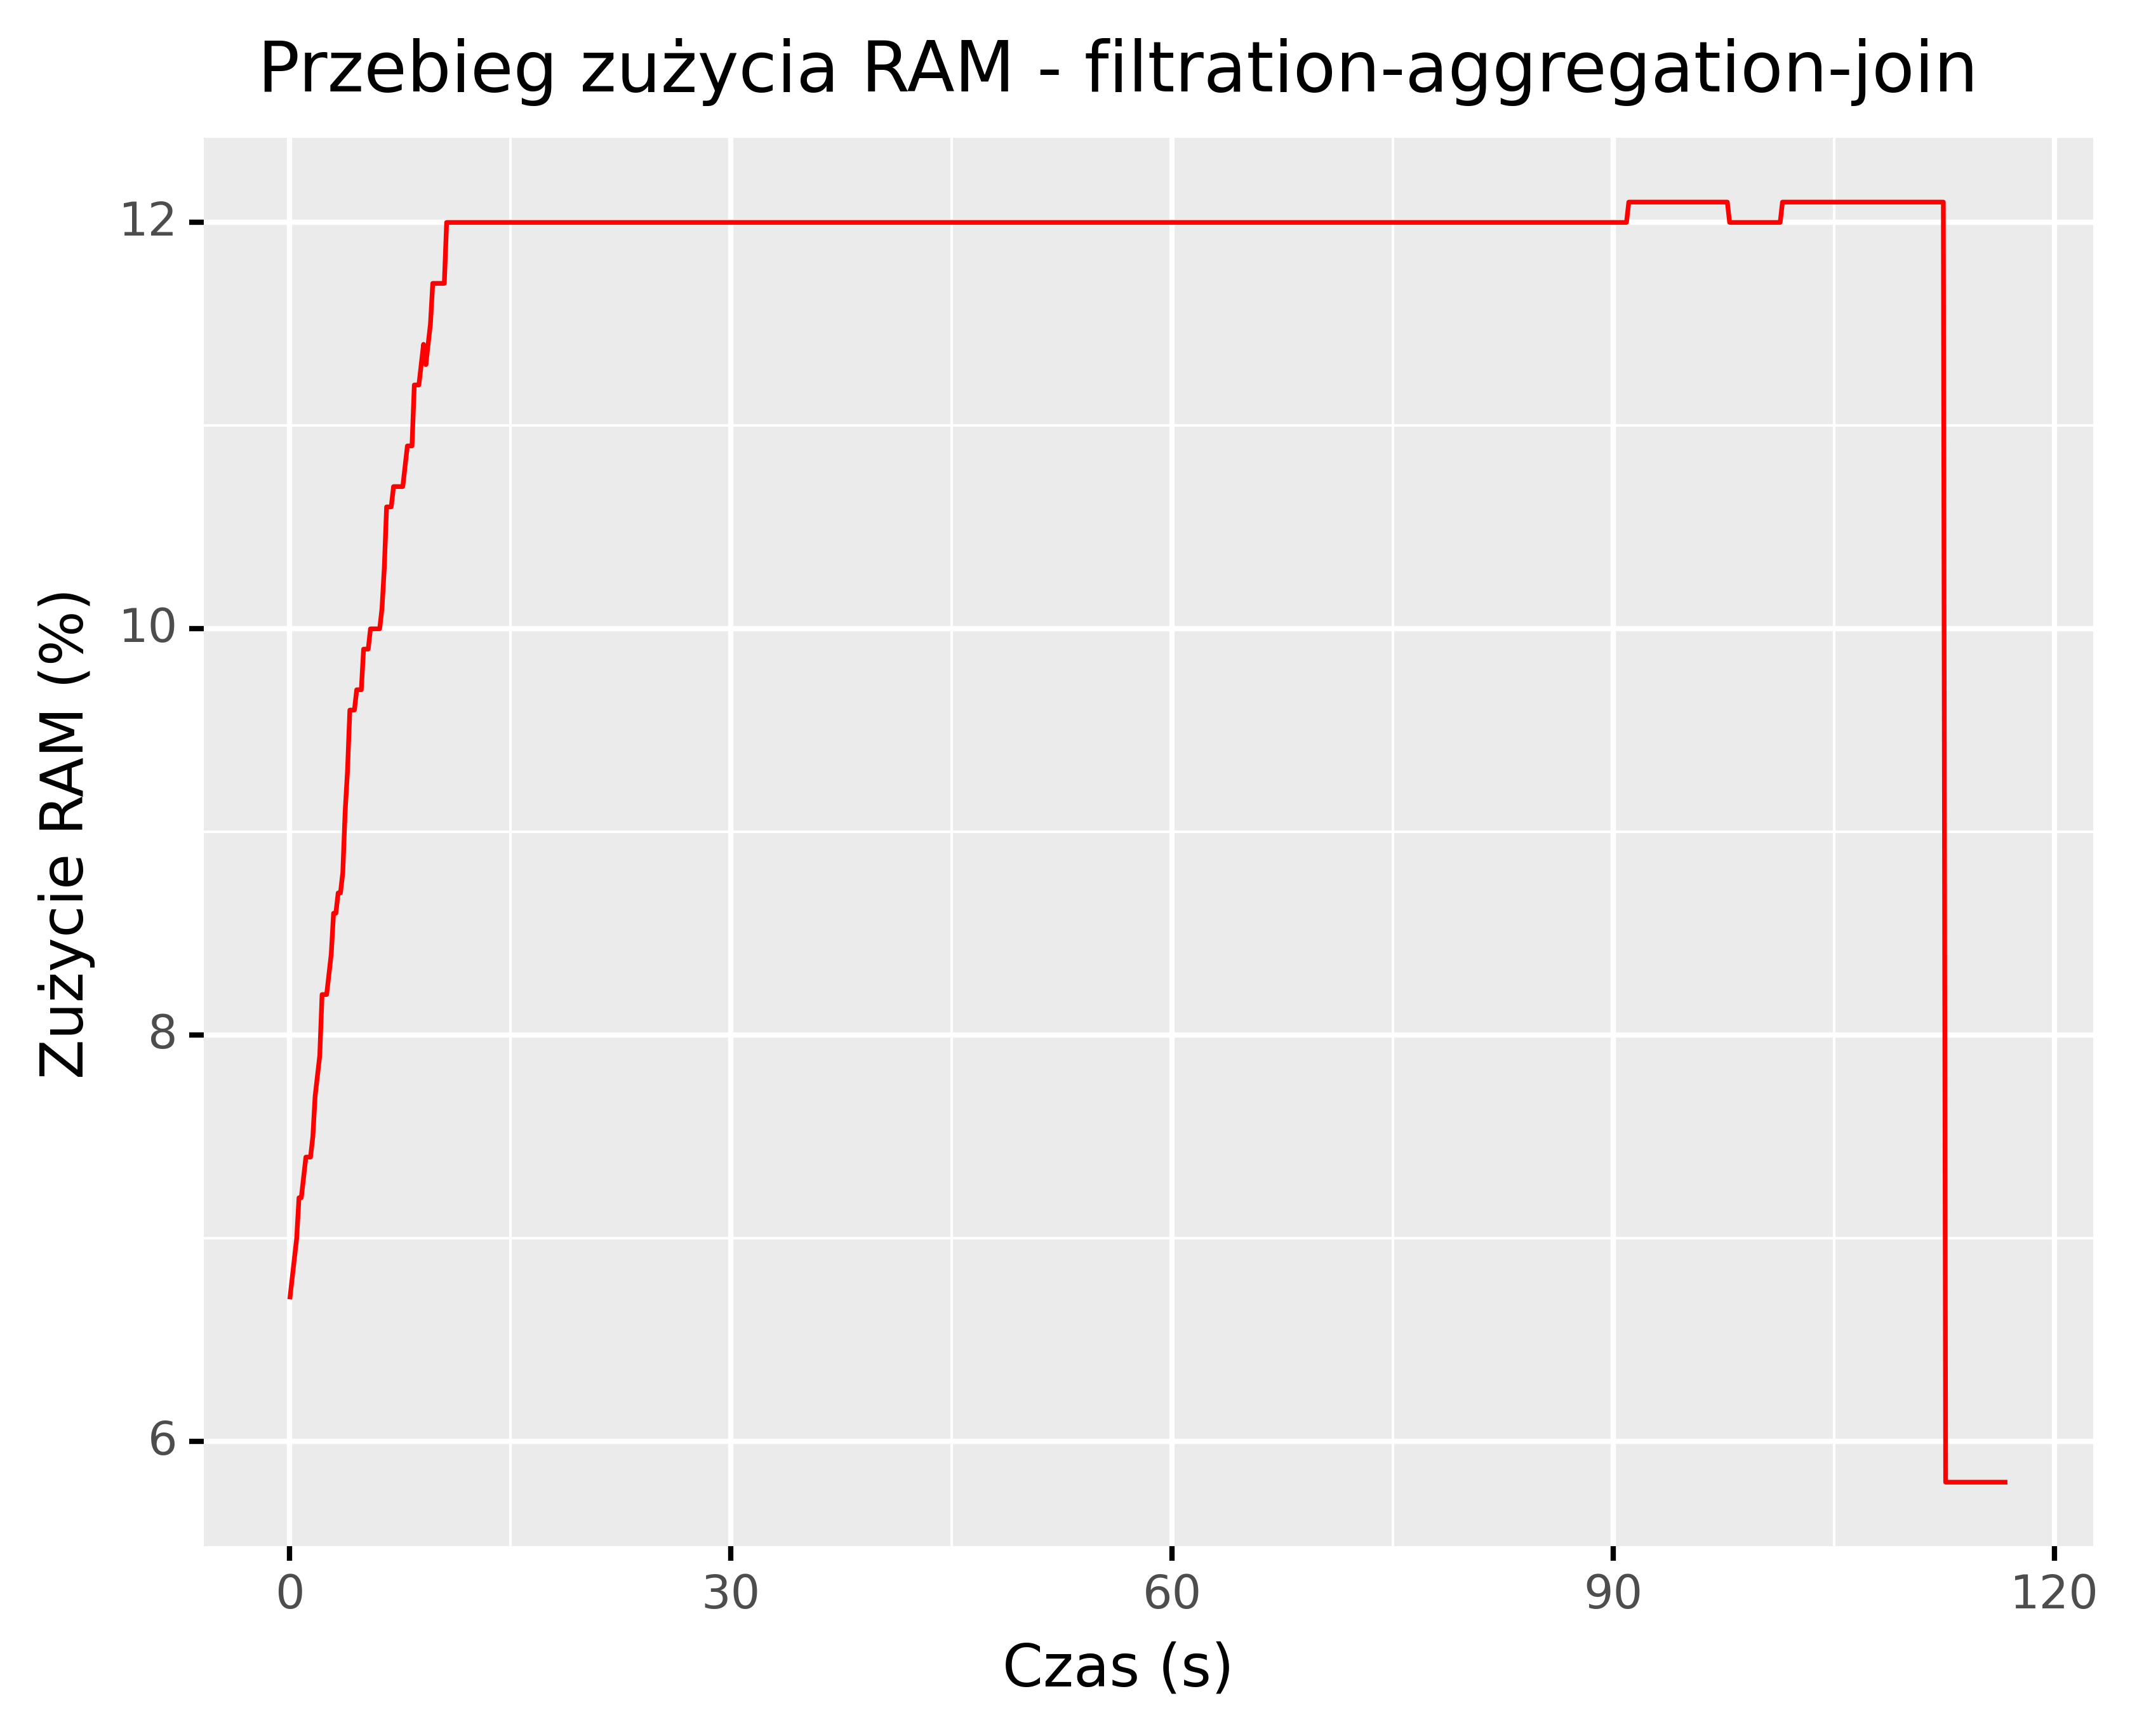
\includegraphics[width=0.5\textwidth]{figures/04-opis-danych/filtration-aggregation-join_example_ram_snapshot_1.png}\label{filtration-aggregation-join:f2}}
  \caption{Przykładowy przebieg zużycia zasobów dla filtracjo-agregacji z połączeniem (snapshot = 1)}
  \label{filtration-aggregation-join_example}
\end{figure}

\begin{figure}[!h]
  \centering
  \subfloat[CPU]{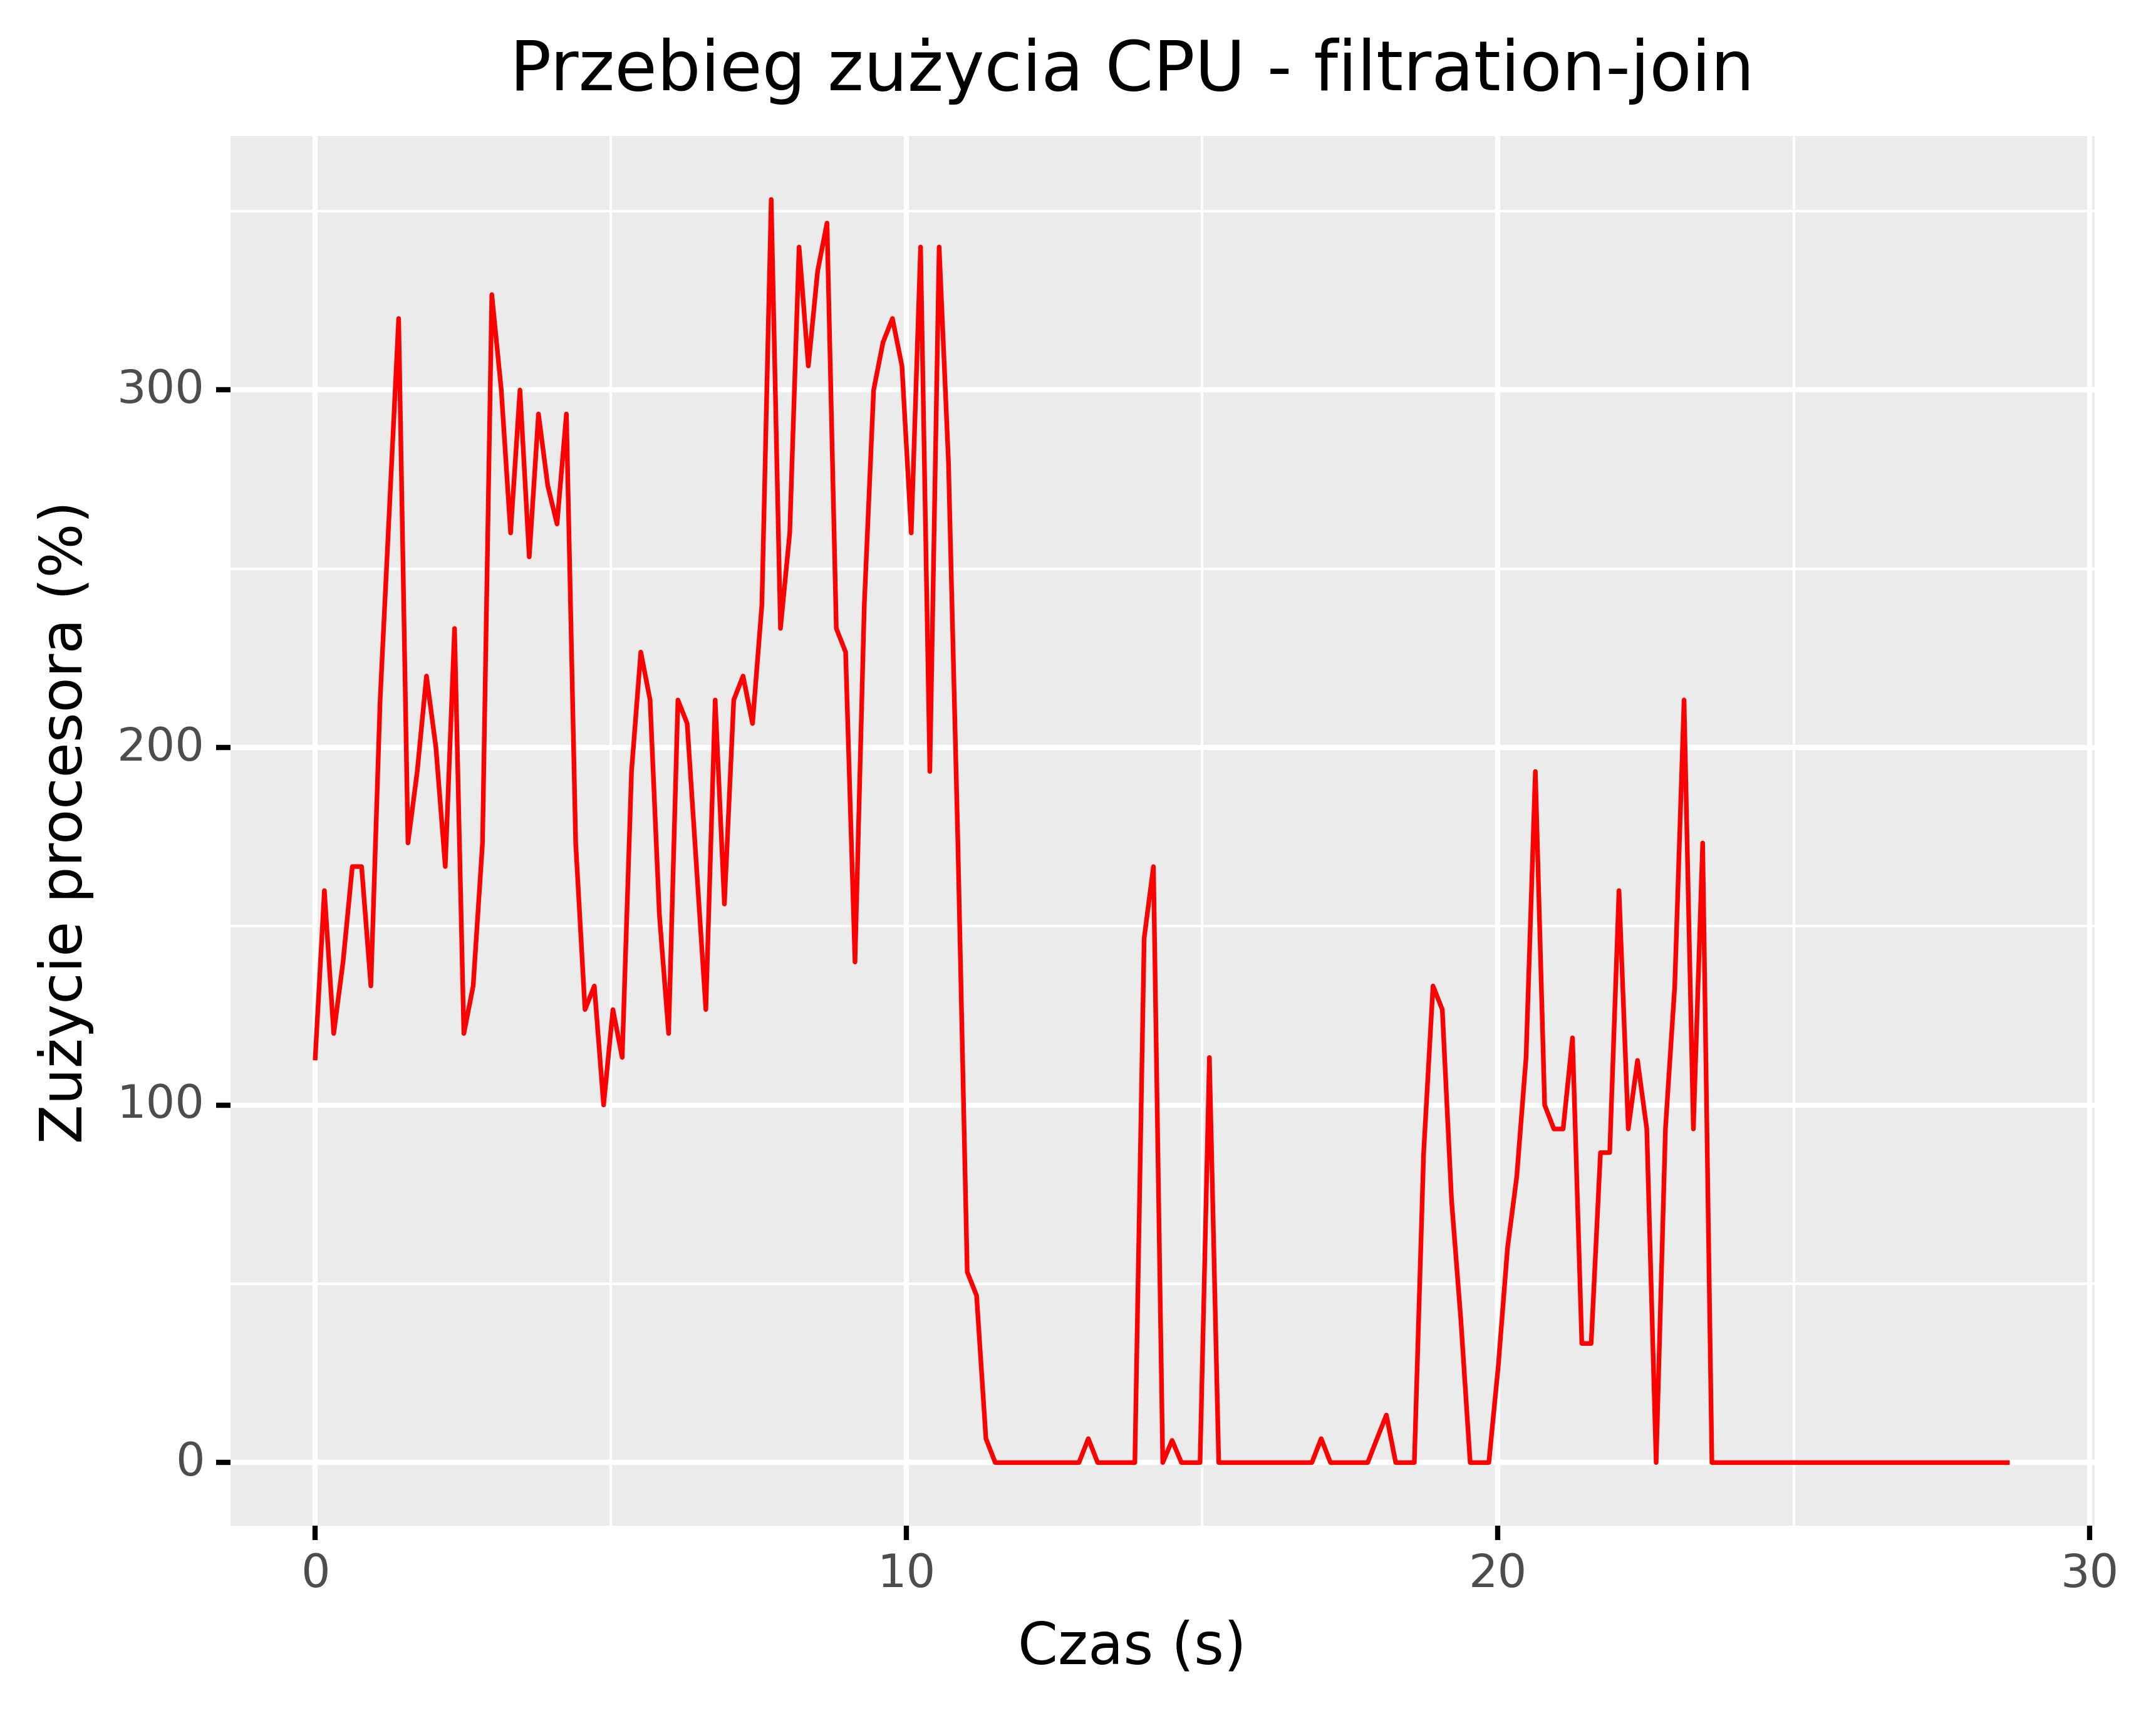
\includegraphics[width=0.5\textwidth]{figures/04-opis-danych/filtration-join_example_cpu_snapshot_1.png}\label{filtration-join_example:f1}}
  \hfill
  \subfloat[RAM]{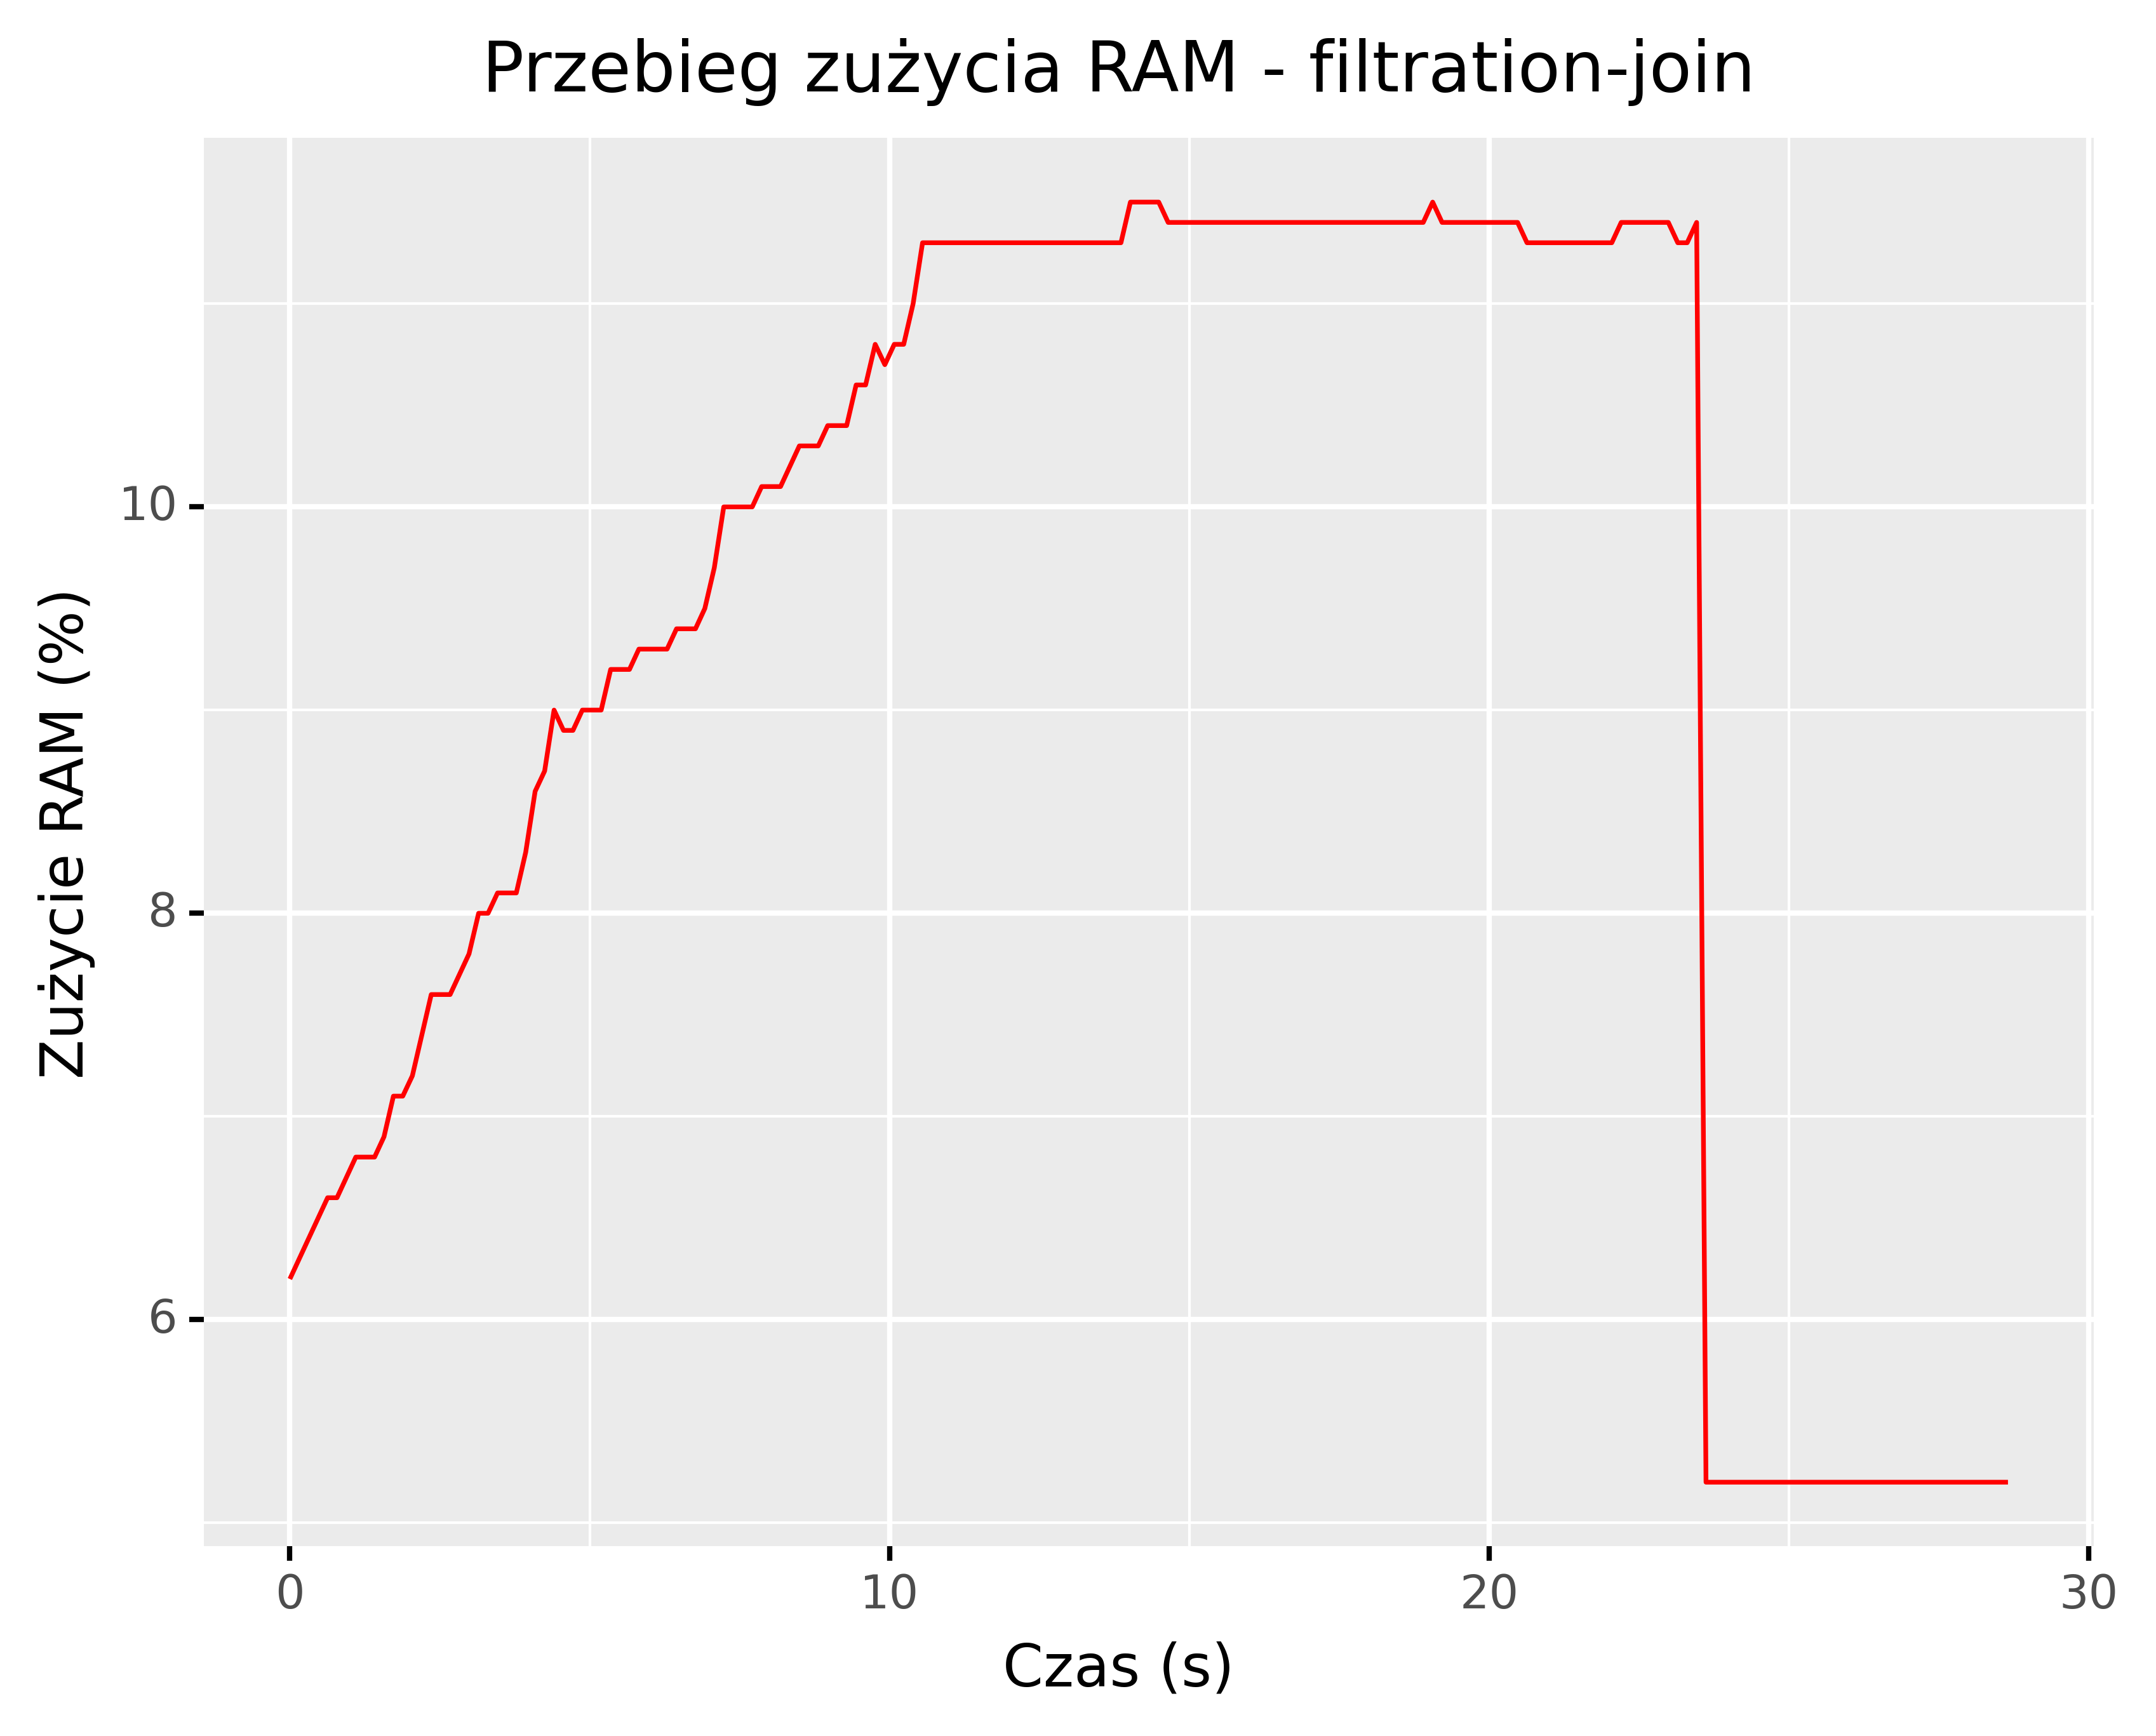
\includegraphics[width=0.5\textwidth]{figures/04-opis-danych/filtration-join_example_ram_snapshot_1.png}\label{filtration-join_example:f2}}
  \caption{Przykładowy przebieg zużycia zasobów dla filtracji z połączeniem (snapshot = 1)}
  \label{filtration-join_example}
  
\end{figure}

Na rysunkach \ref{aggregation_example} do \ref{filtration-join_example} widać, że wykresy CPU są bardzo ostre i mogły by zyskać na wygładzeniu krawędzi. Wykonaliśmy to przy użyciu średniej w oknie przesuwnym. Okno brało pod uwagę liczbę próbek zależną od tego jak dużo okno czasowe chcemy brać pod uwagę. Próbki są zebrane w odstępach 0.15 sekundy, więc ok sześciu próbek równe jest jednej sekundzie. Poniżej znajdują się wykresy przestawiający wygląd wykresów po wygładzeniu dla różnej liczby próbek dla przykładowego przebiegu agregacji.

\begin{figure}[H]
  \centering
  \subfloat[CPU]{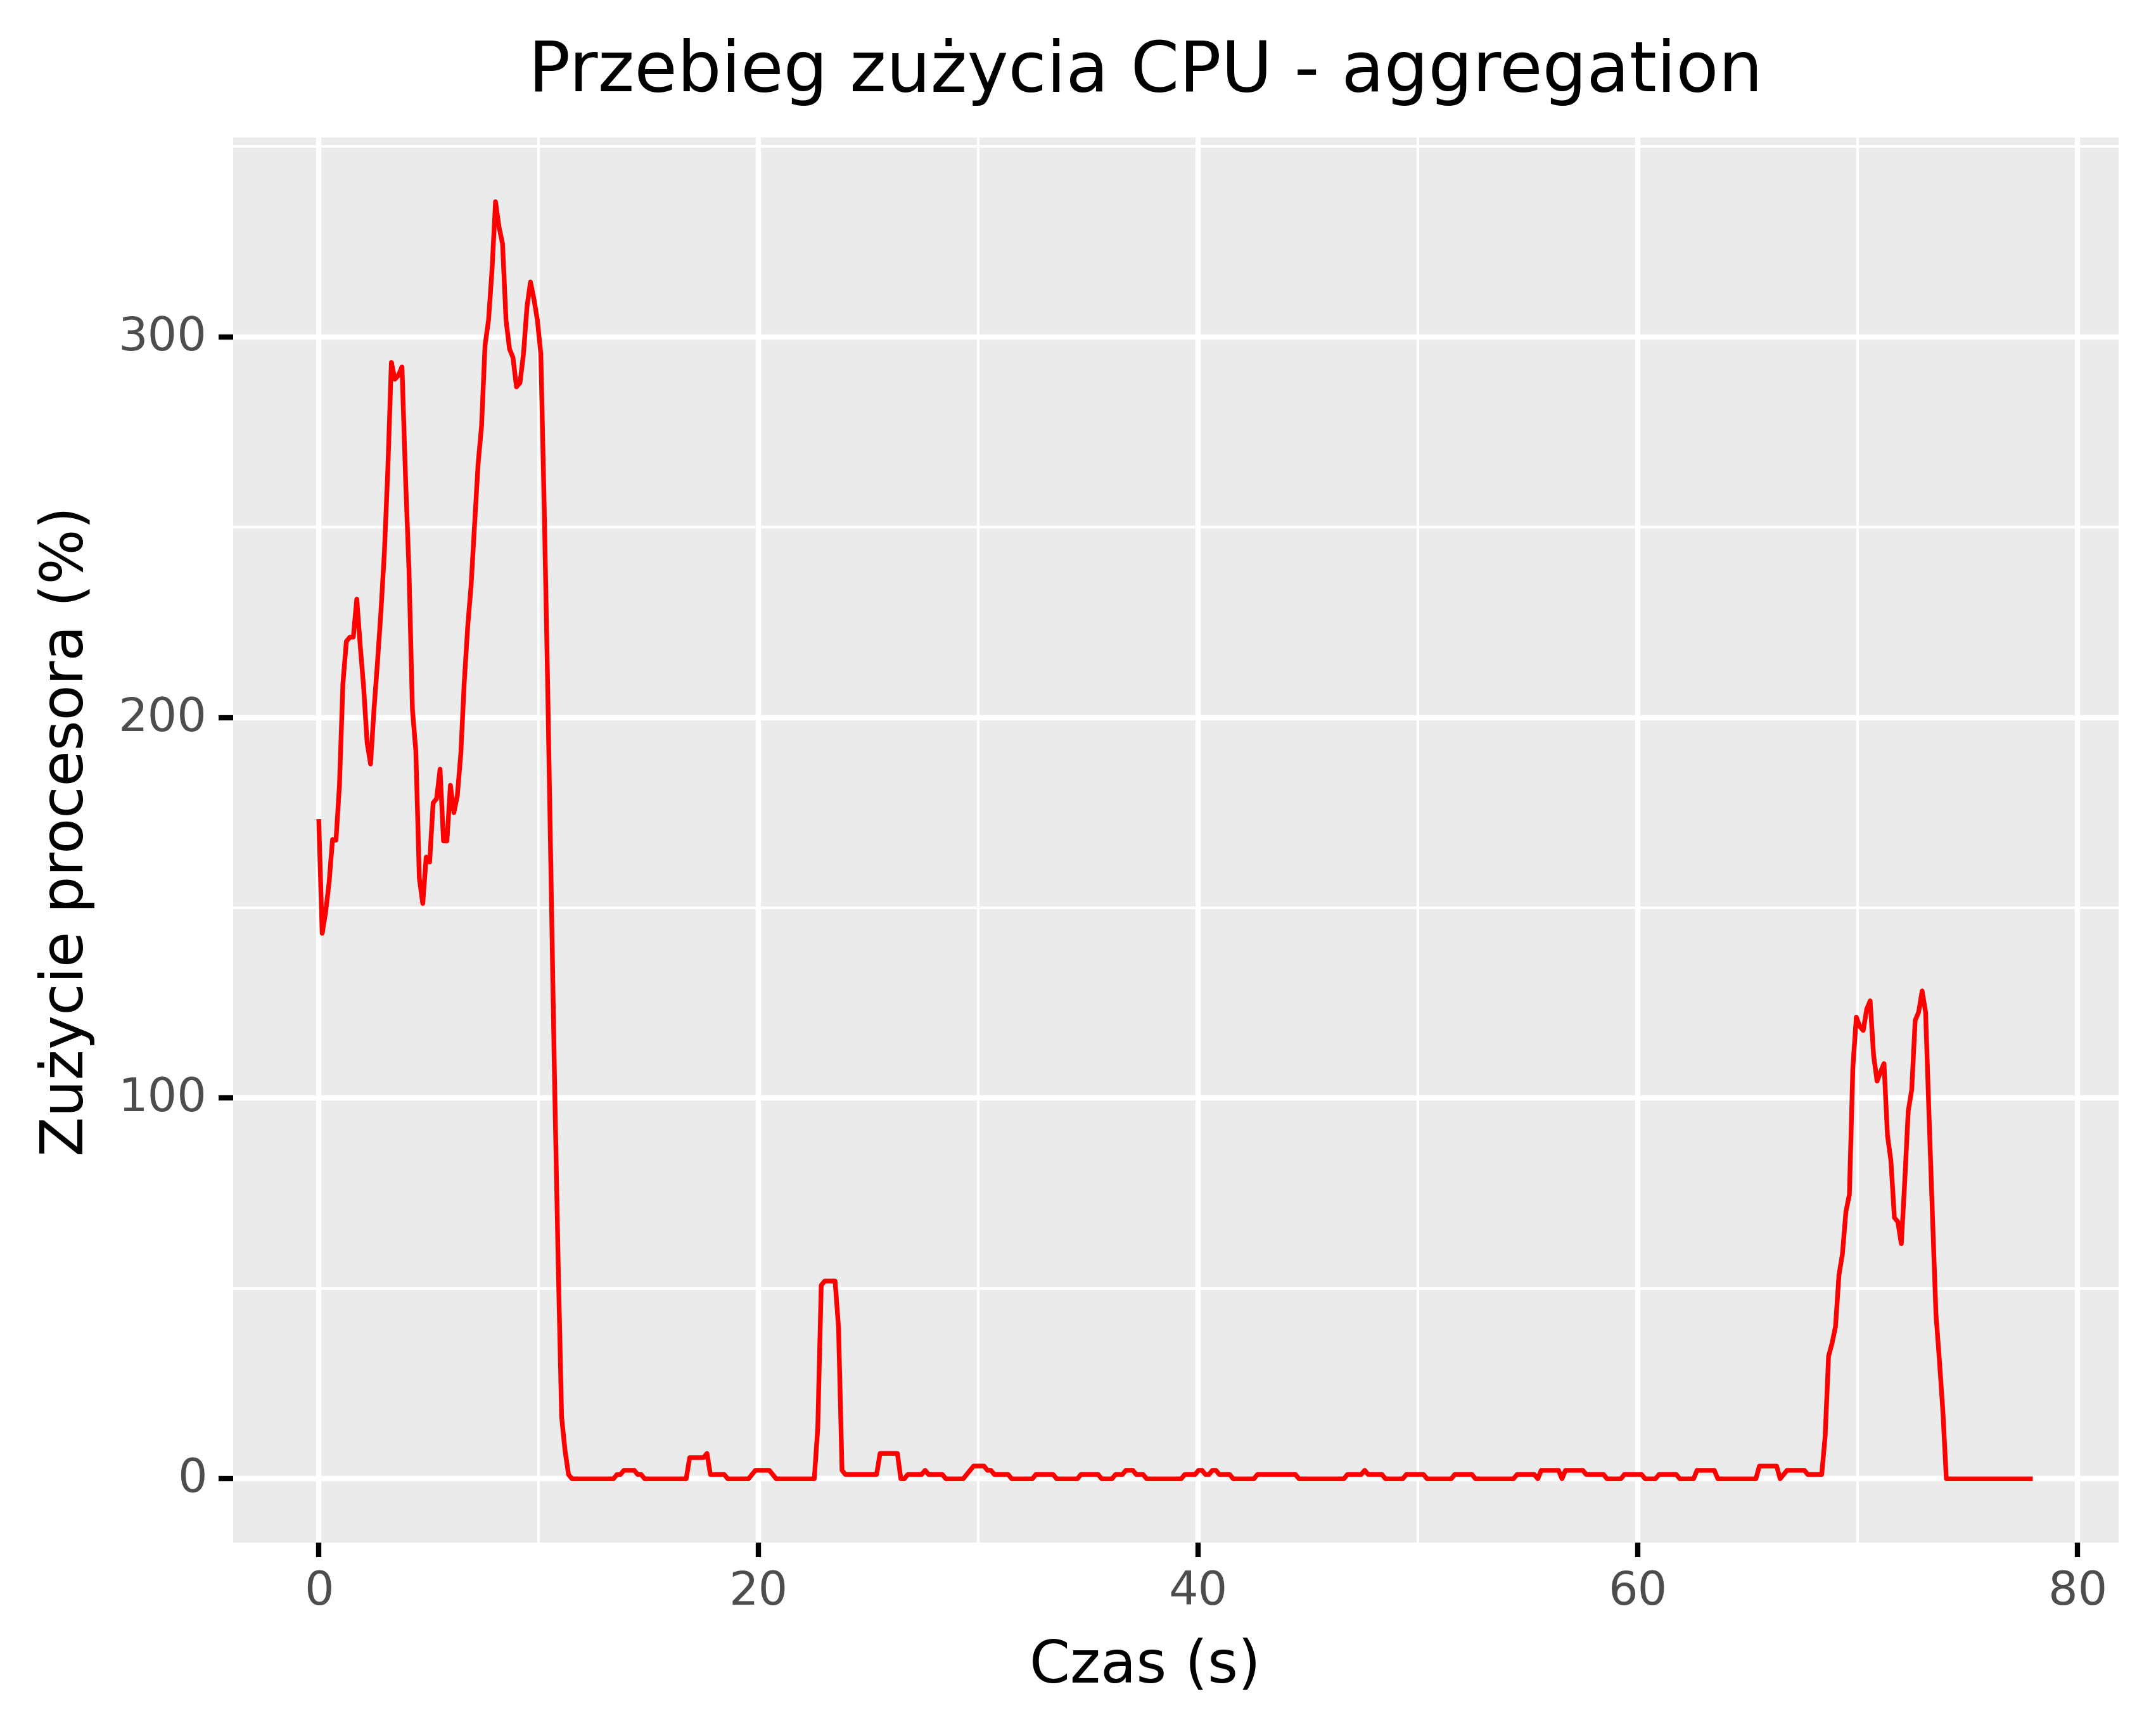
\includegraphics[width=0.5\textwidth]{figures/04-opis-danych/aggregation_smooth_6_cpu_snapshot_1.png}\label{aggregation_smooth_6:f1}}
  \hfill
  \subfloat[RAM]{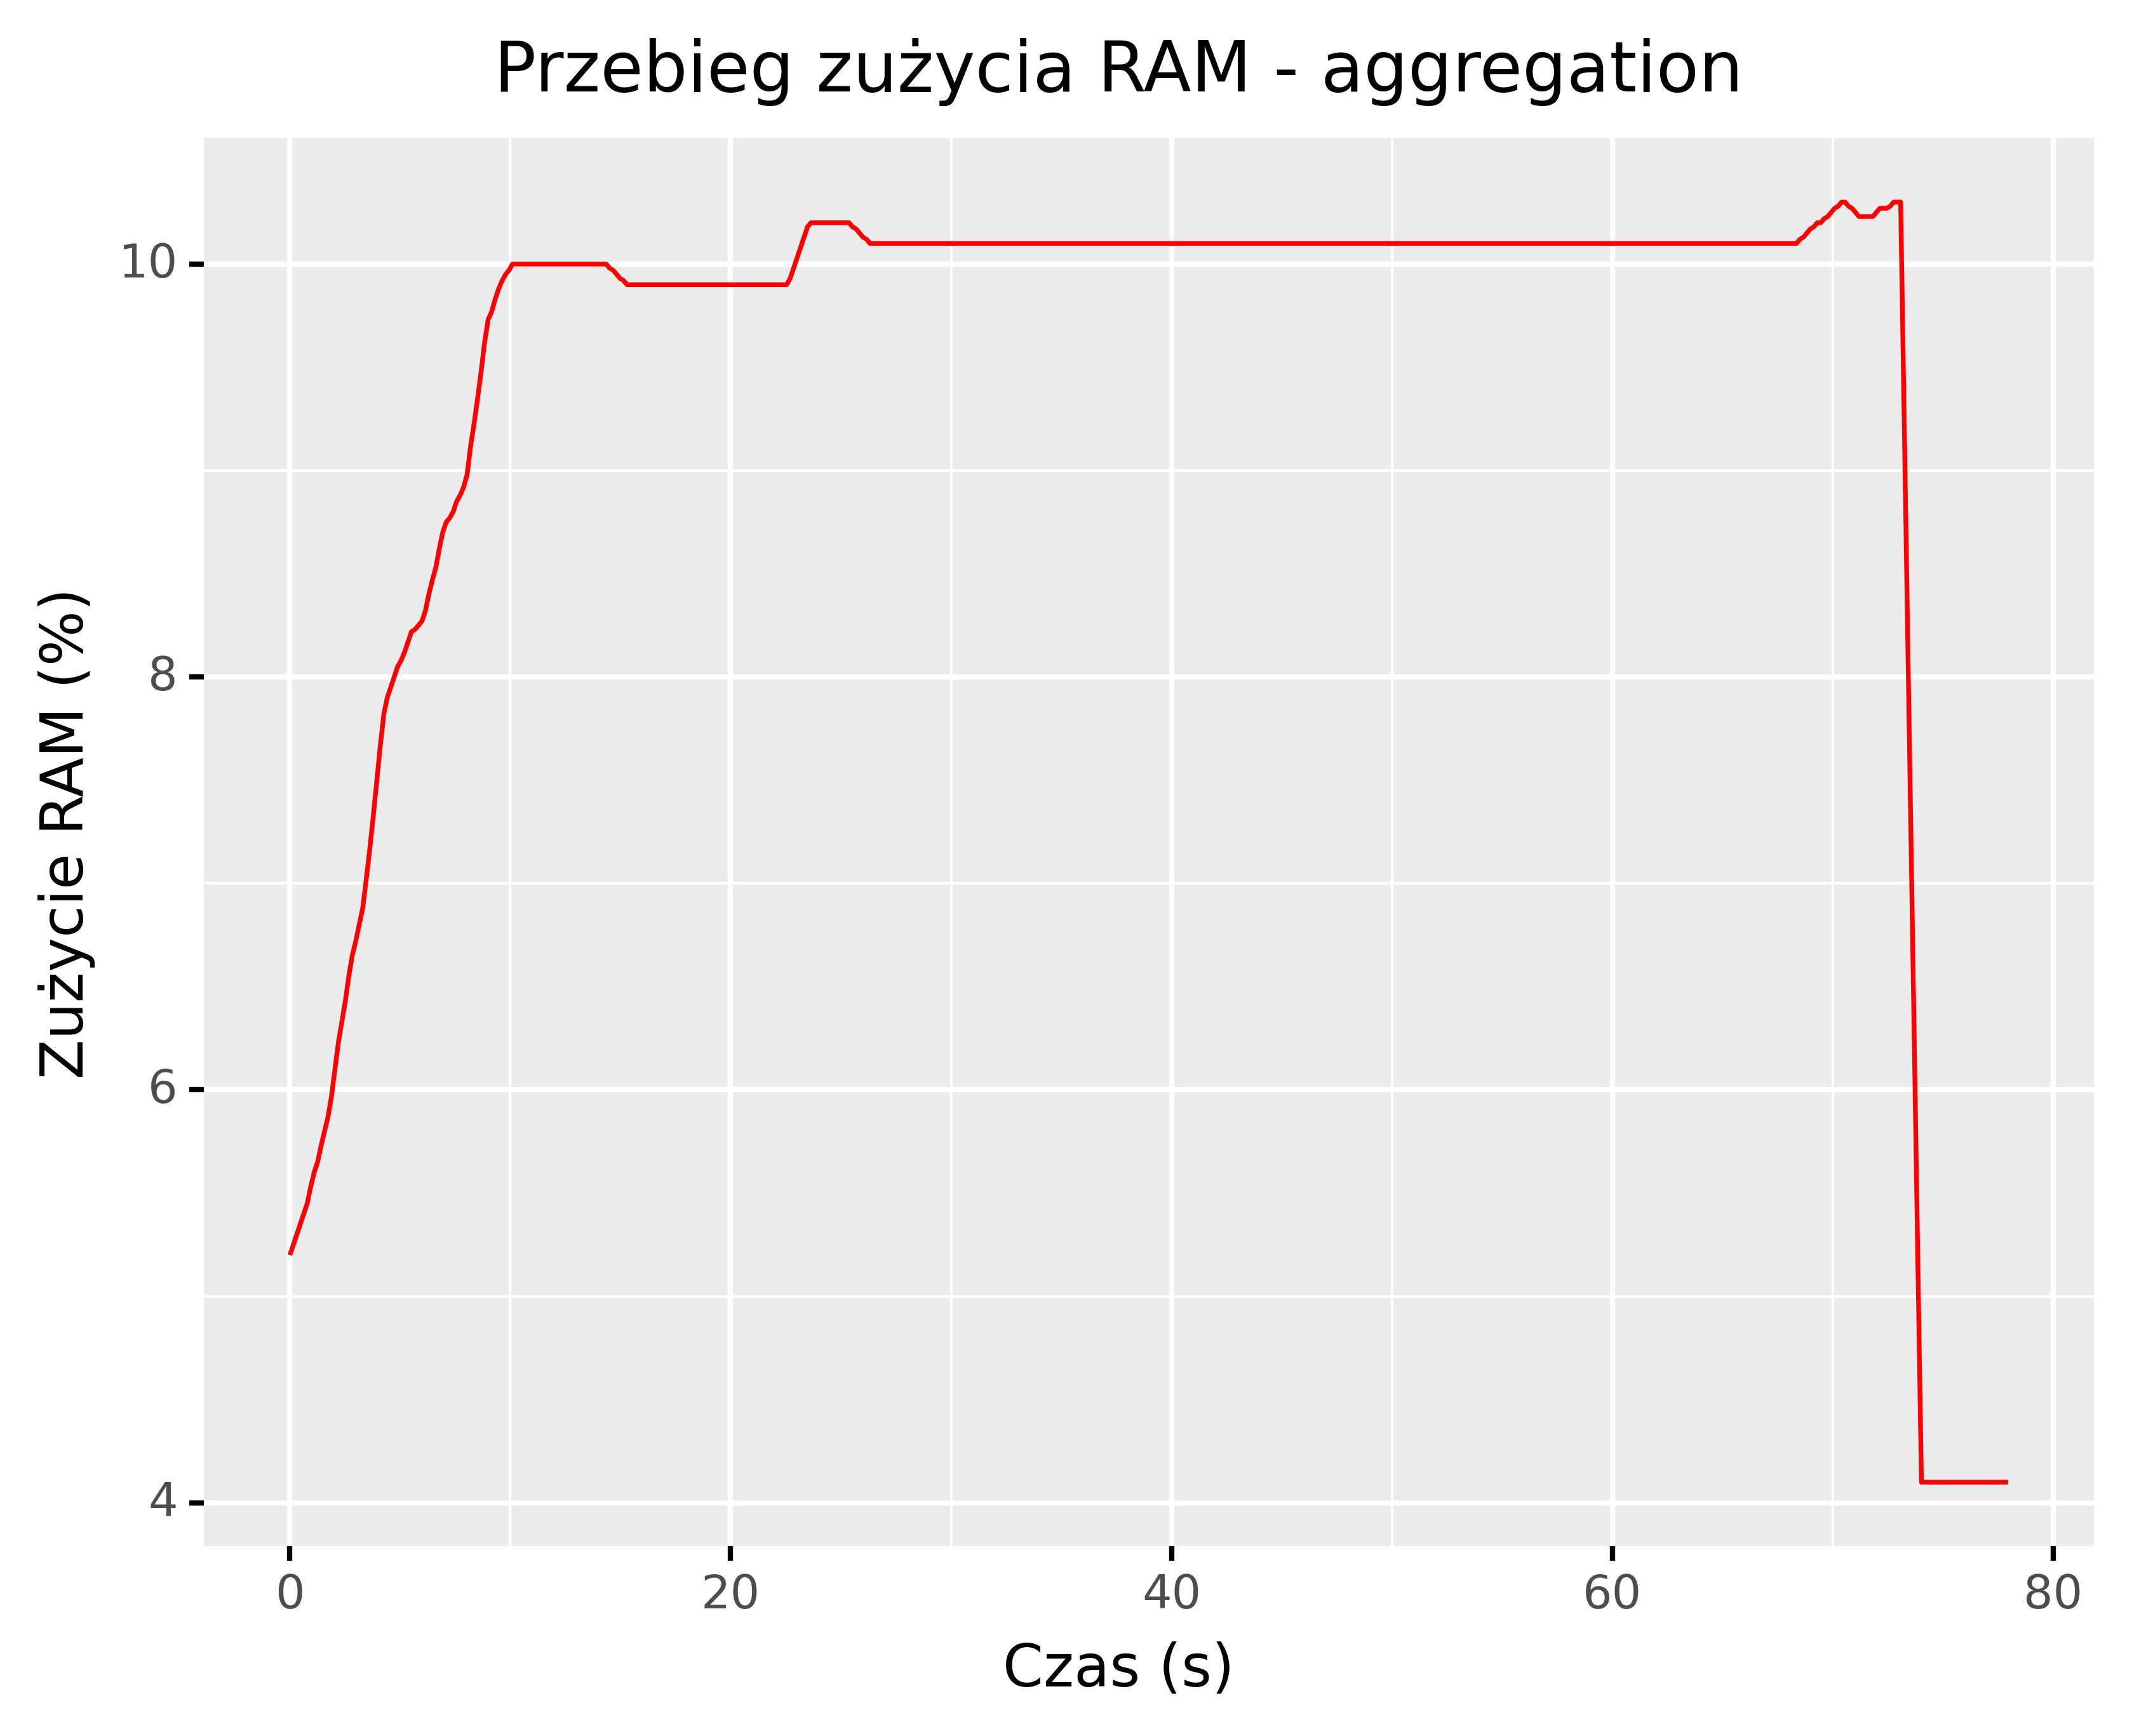
\includegraphics[width=0.5\textwidth]{figures/04-opis-danych/aggregation_smooth_6_ram_snapshot_1.png}\label{aggregation_smooth_6:f2}}
  \caption{Przykładowy wygładzony wykres zużycia zasobów dla agregacji (snapshot = 1, okno 1 sekundowe)}
  \label{aggregation_smooth_6}
\end{figure}

\begin{figure}[H]
  \centering
  \subfloat[CPU]{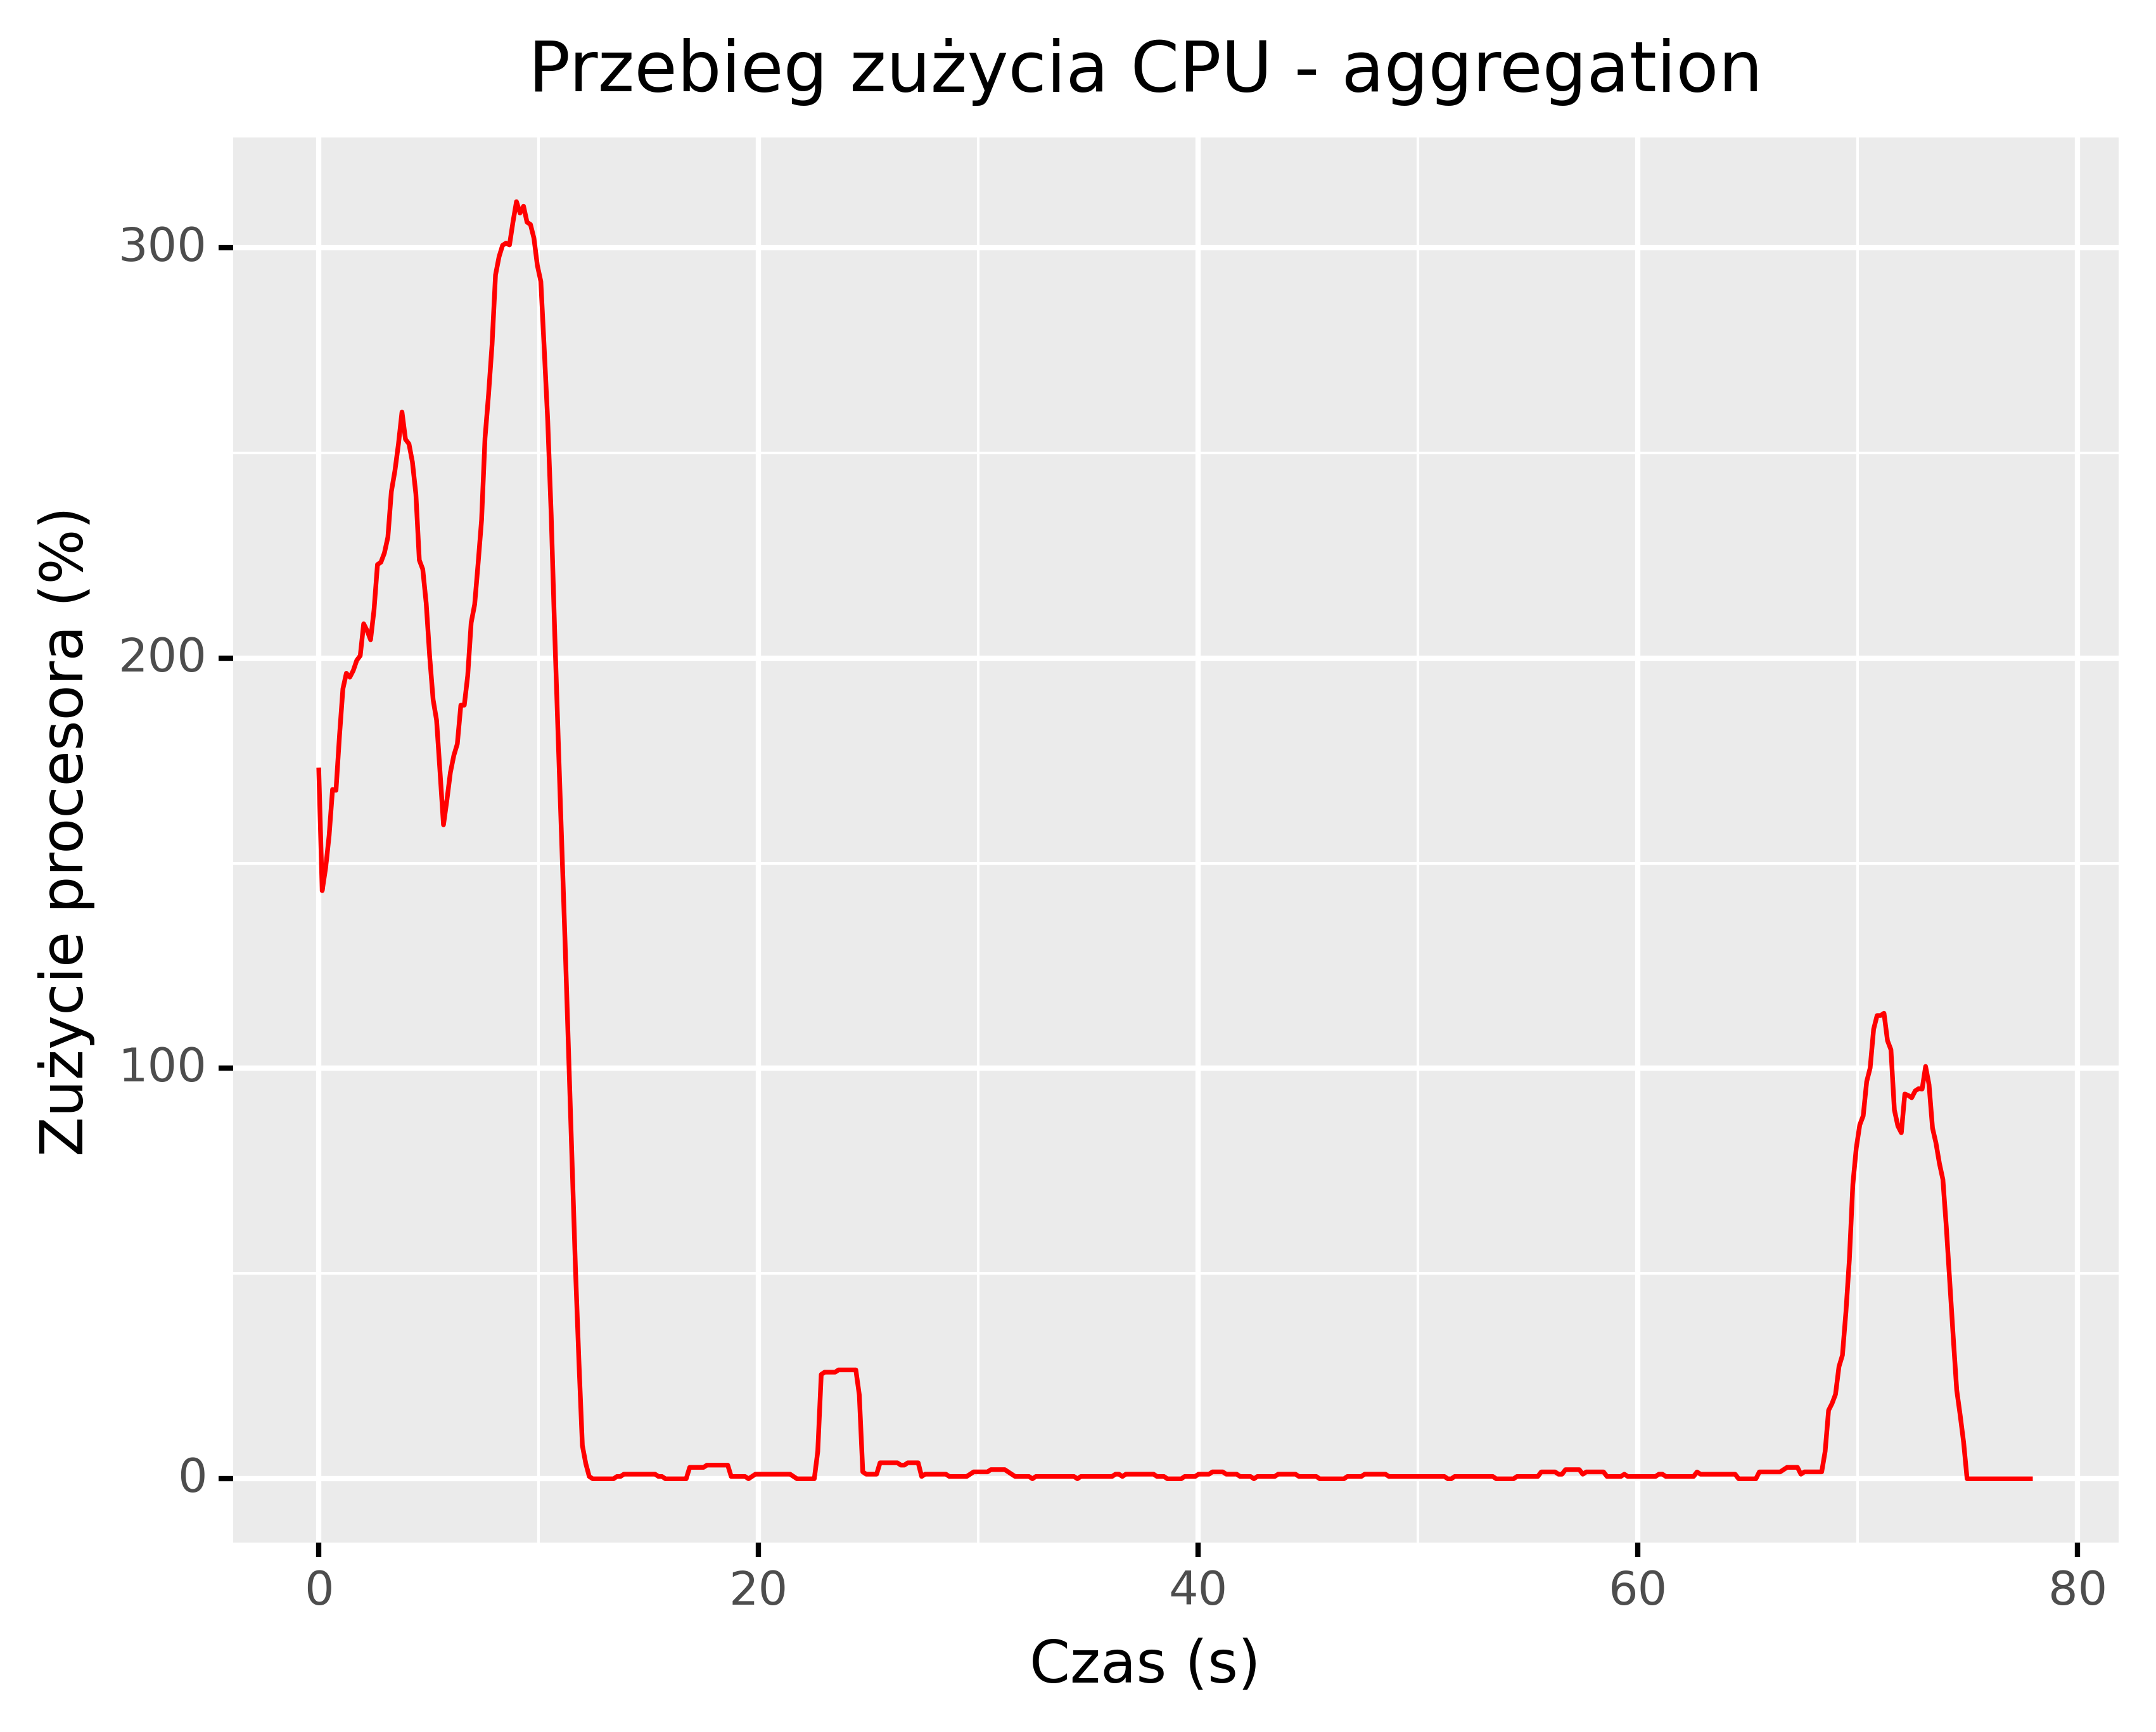
\includegraphics[width=0.5\textwidth]{figures/04-opis-danych/aggregation_smooth_12_cpu_snapshot_1.png}\label{aggregation_smooth_12:f1}}
  \hfill
  \subfloat[RAM]{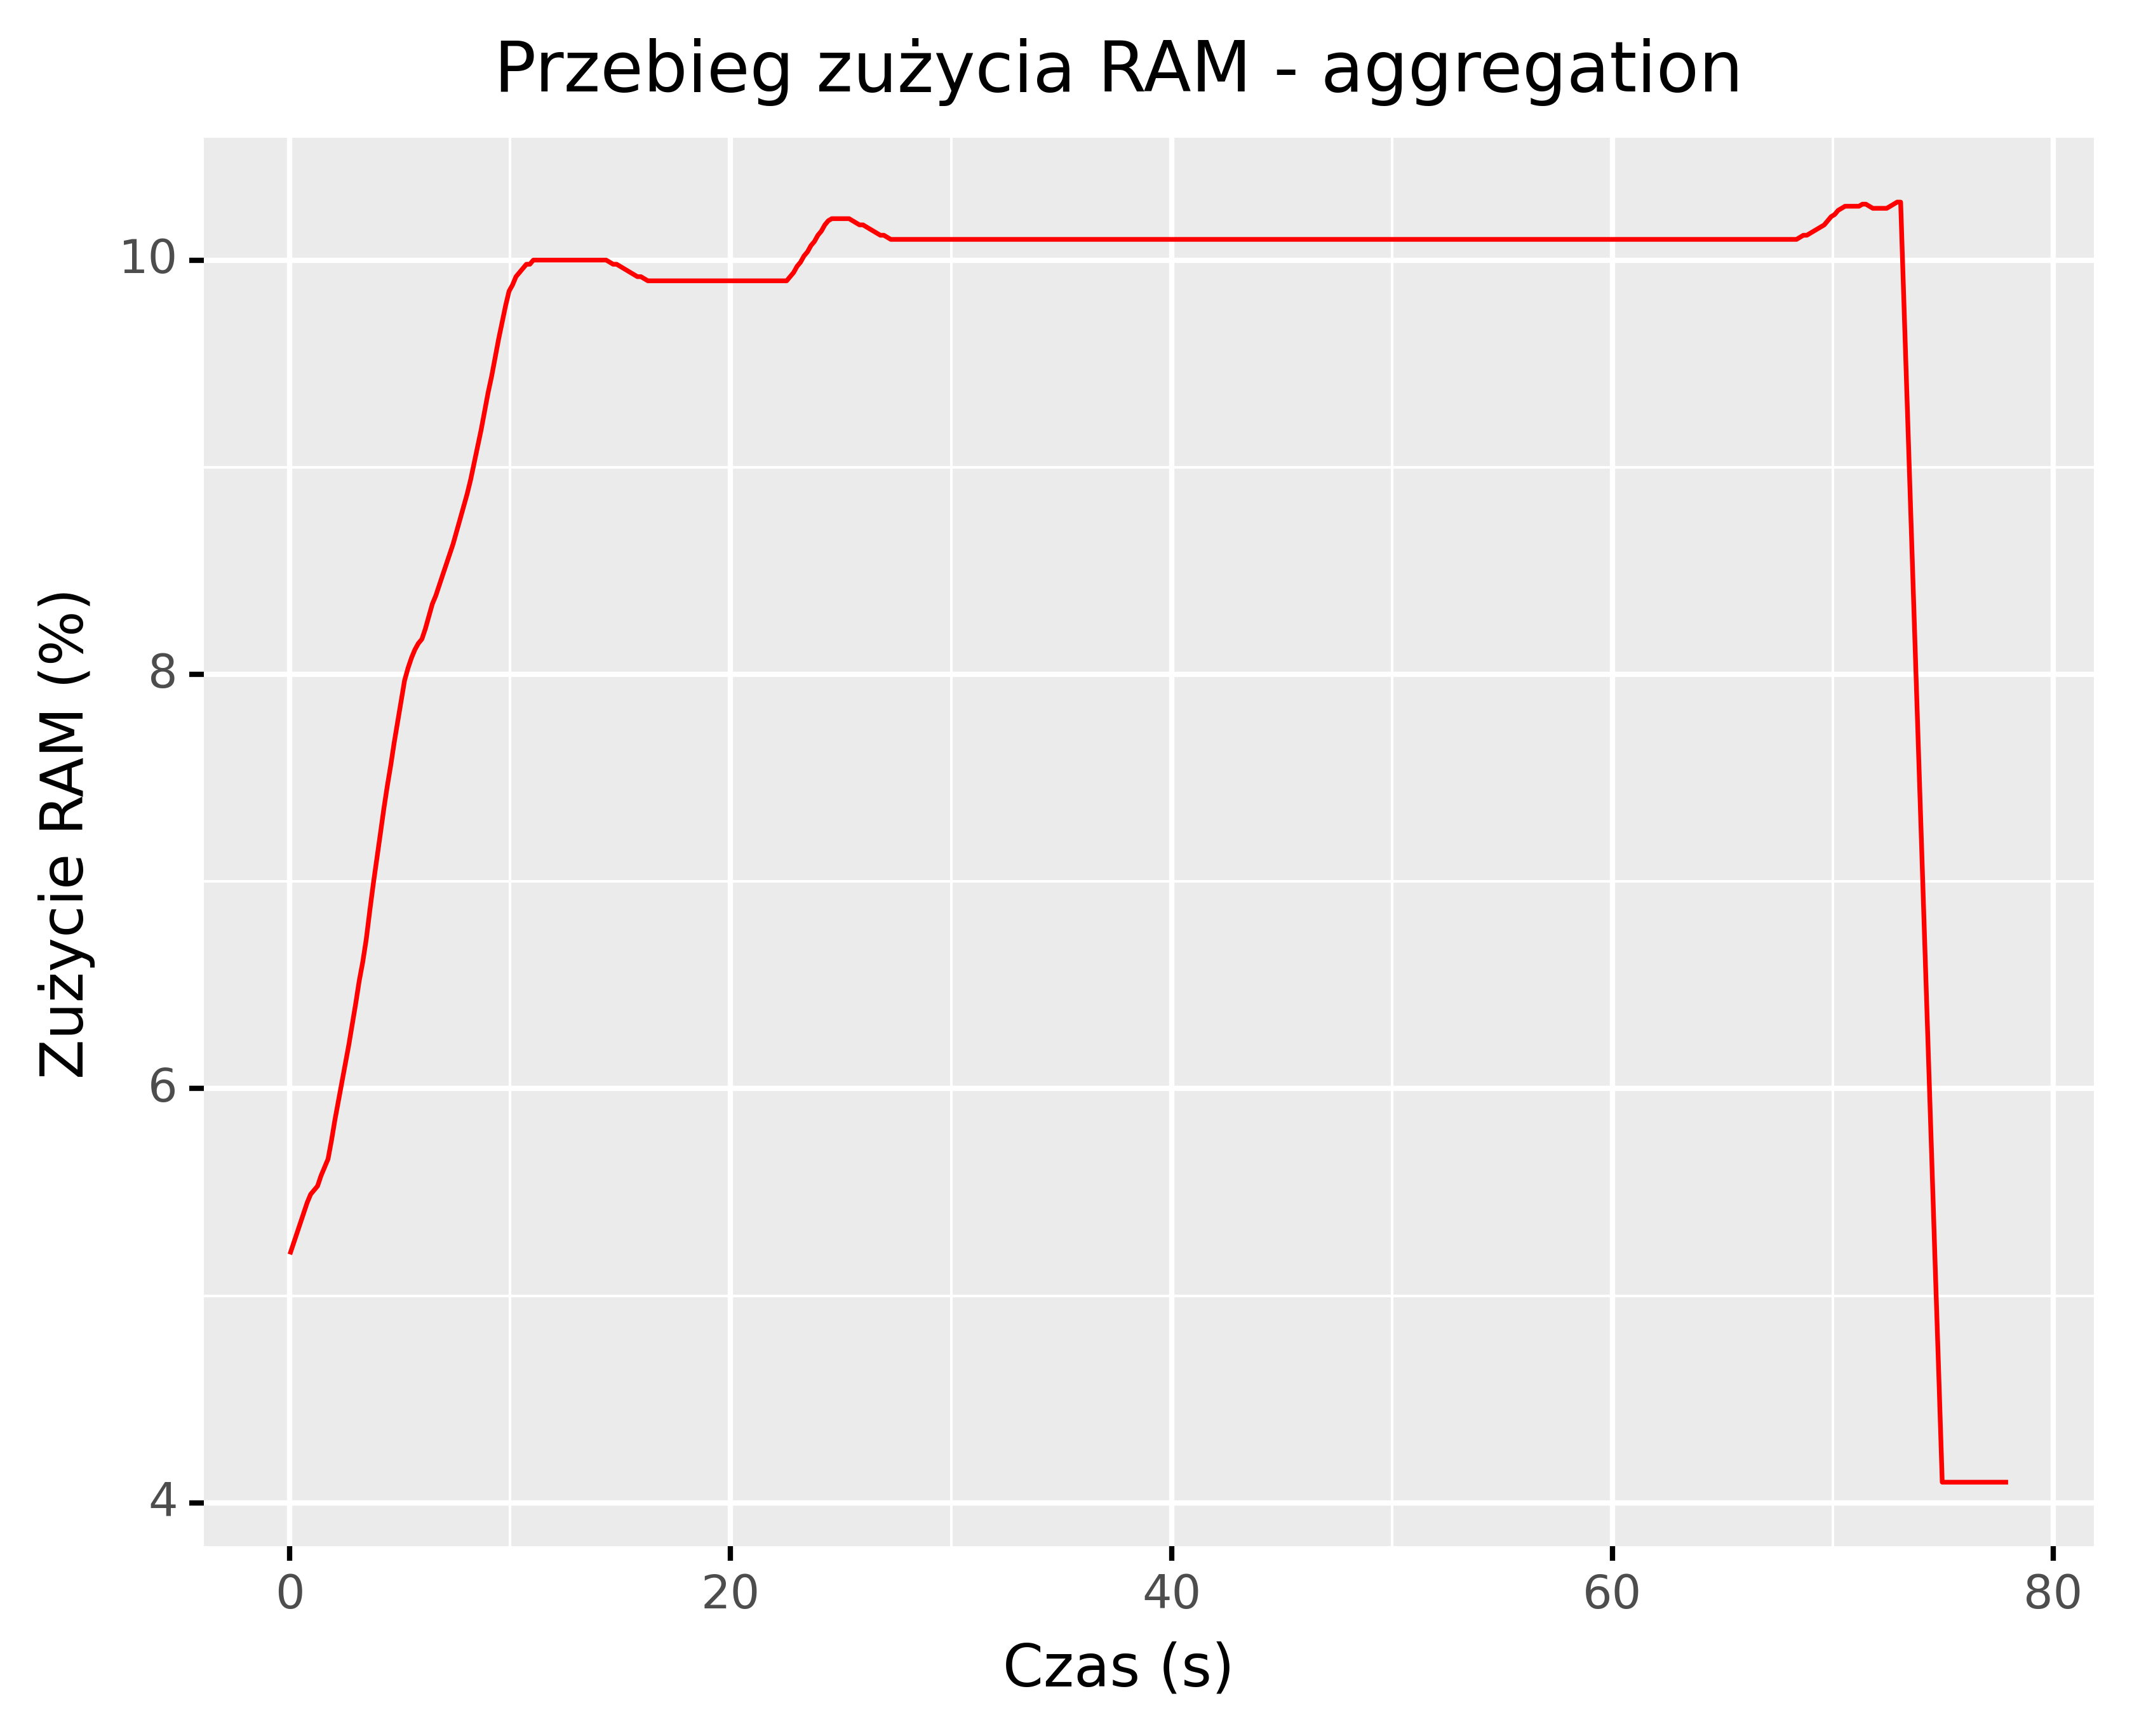
\includegraphics[width=0.5\textwidth]{figures/04-opis-danych/aggregation_smooth_12_ram_snapshot_1.png}\label{aggregation_smooth_12:f2}}
  \caption{Przykładowy wygładzony wykres zużycia zasobów dla agregacji (snapshot = 1, okno 2 sekundowe)}
  \label{aggregation_smooth_12}
\end{figure}

\begin{figure}[H]
  \centering
  \subfloat[CPU]{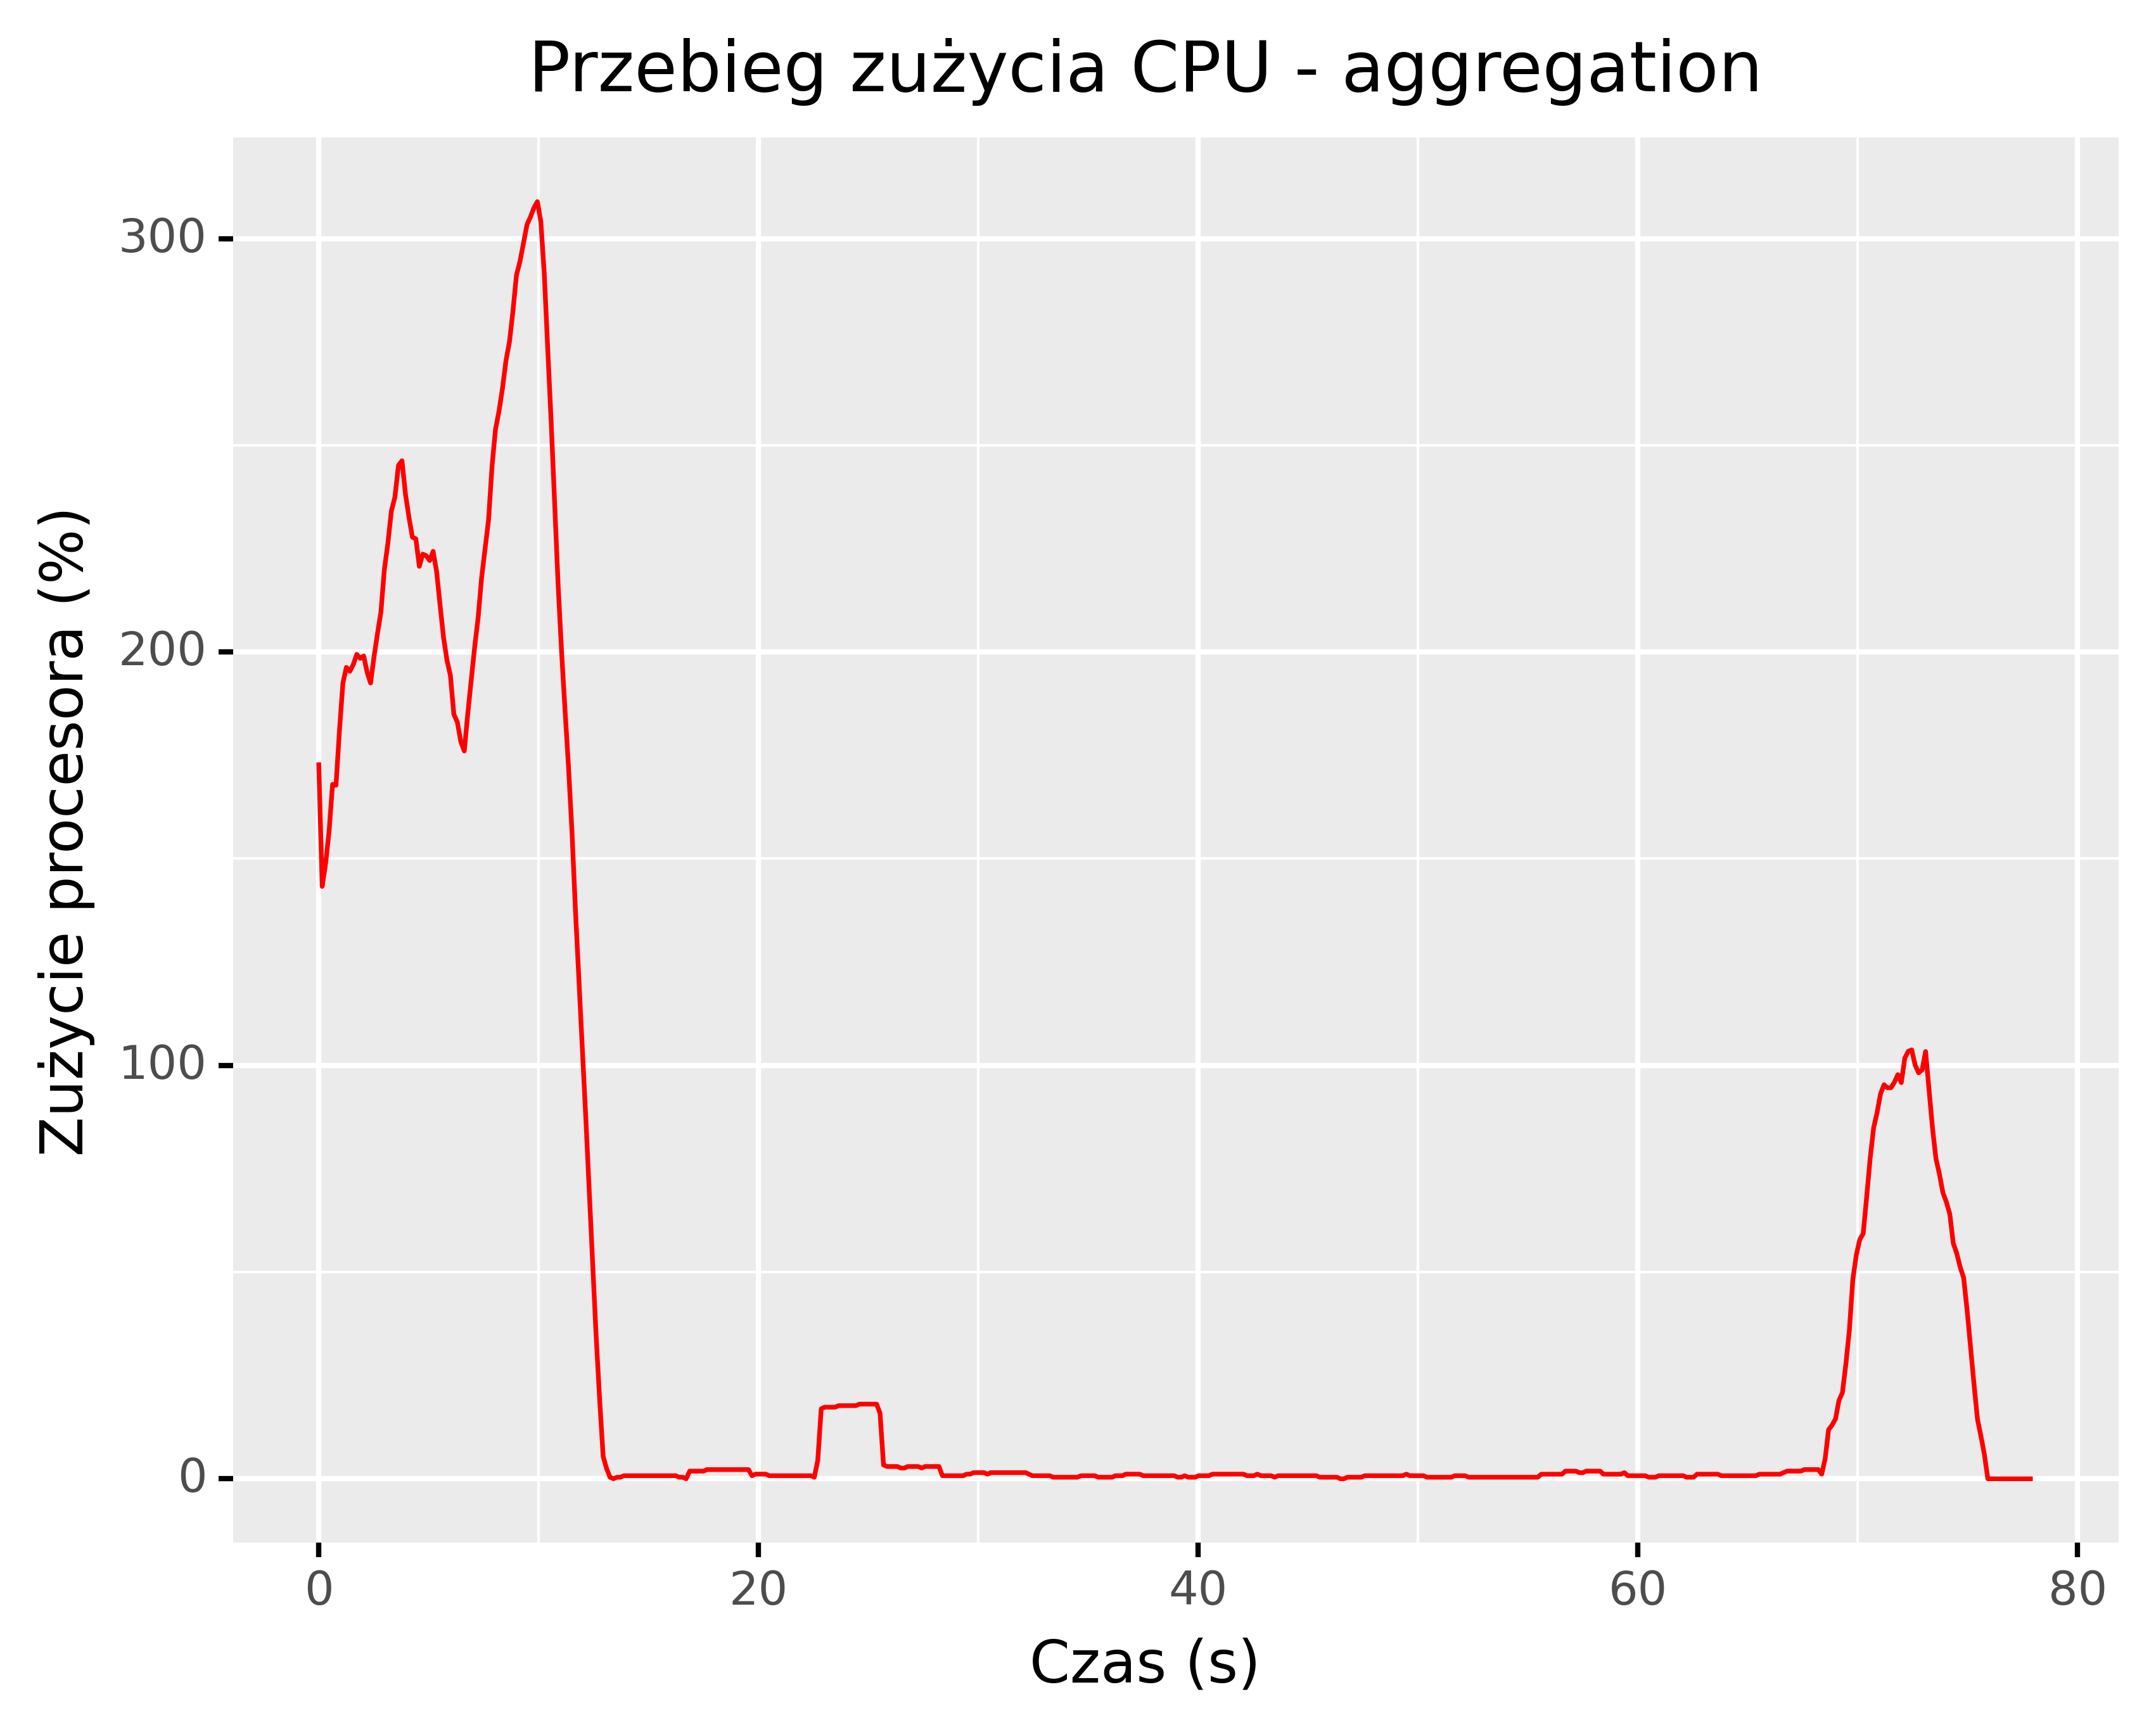
\includegraphics[width=0.5\textwidth]{figures/04-opis-danych/aggregation_smooth_18_cpu_snapshot_1.png}\label{aggregation_smooth_18:f1}}
  \hfill
  \subfloat[RAM]{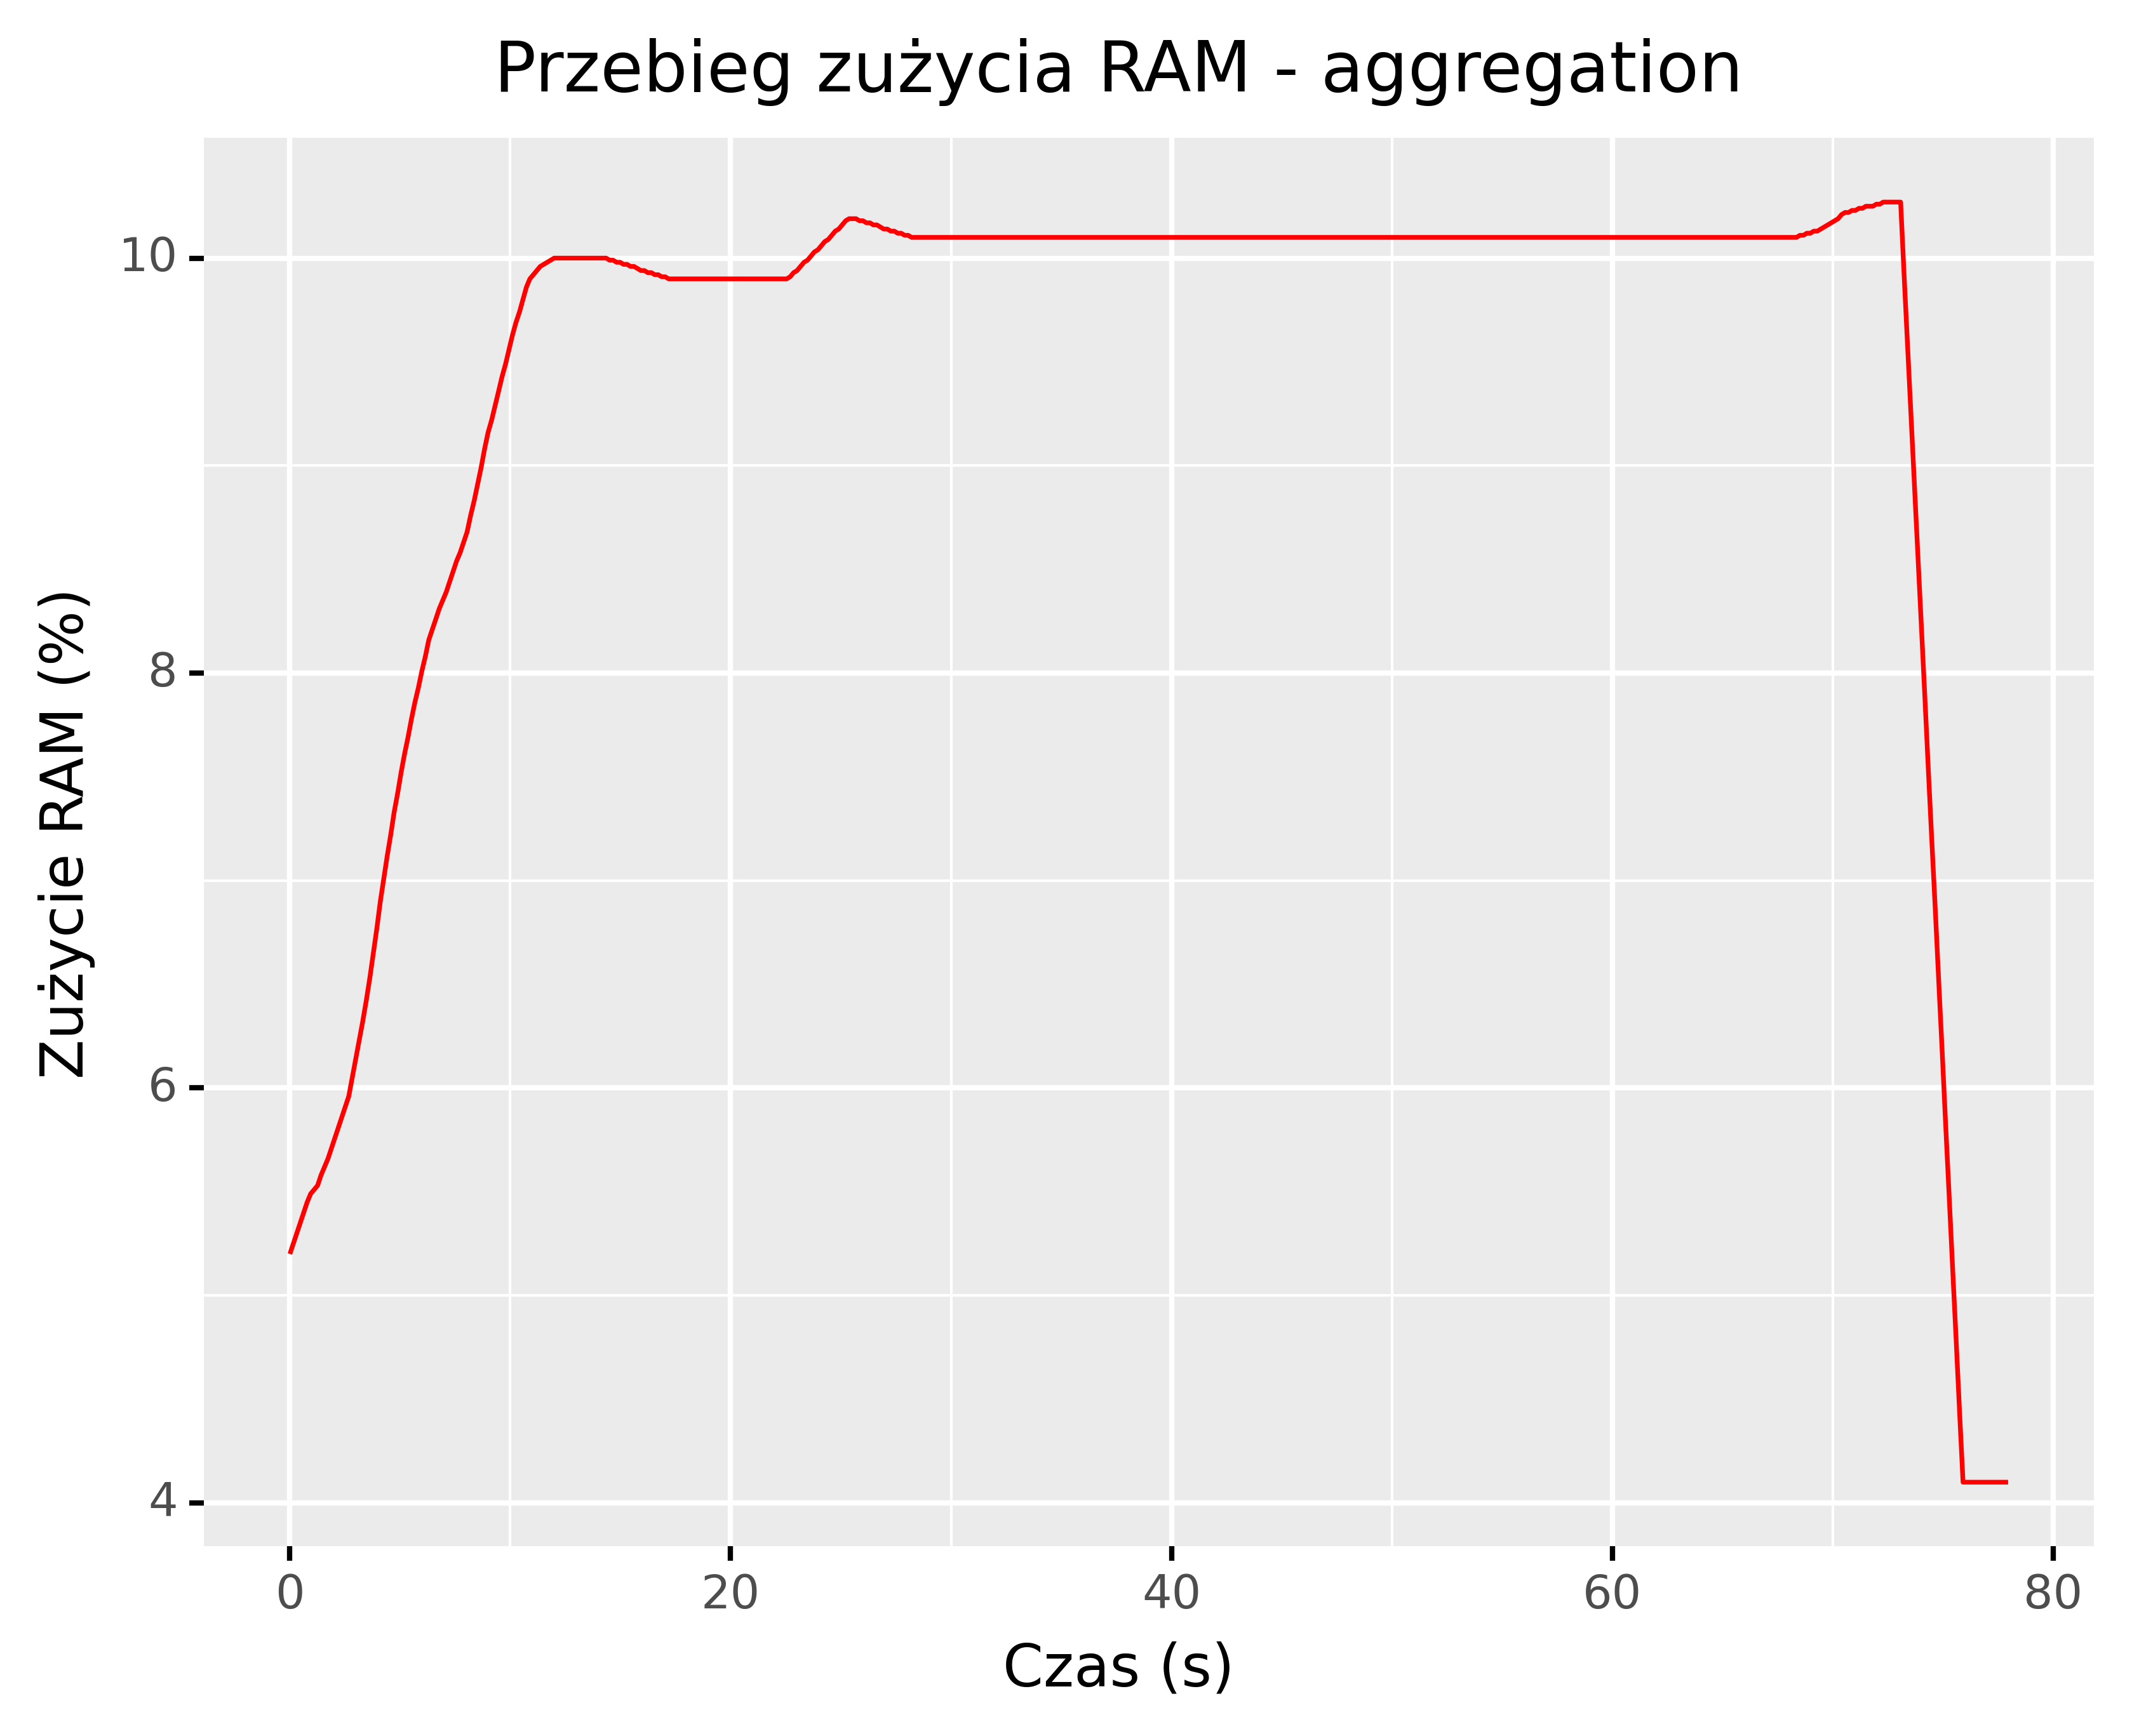
\includegraphics[width=0.5\textwidth]{figures/04-opis-danych/aggregation_smooth_18_ram_snapshot_1.png}\label{aggregation_smooth_18:f2}}
  \caption{Przykładowy wygładzony wykres zużycia zasobów dla agregacji (snapshot = 1, okno 3 sekundowe)}
  \label{aggregation_smooth_18}
\end{figure}

Po wykonaniu transformacji można zauważyć, że wykresy są mniej niestabilne (mniej dużej ilości skoków wartości w małym przedziale czasowym). Rysunki od \ref{aggregation_smooth_6} do \ref{aggregation_smooth_18} pokazują na przykładzie agregacji wyniki dla kolejno 6, 12 i 18 próbek (czyli 1, 2, 3 sekundy). Ostatecznie nie chcąc przesadzić będziemy korzystali prawdopodobnie z oknem 1 sekundowym, żeby nie stracić zbyt wielu informacji, co mogłoby się zdarzyć używając zbyt dużego okna. Przykładowo na rysunku CPU \ref{aggregation_smooth_18} widać w porównaniu z rysunkiem \ref{aggregation_smooth_6} mocno zmniejszony szczyt w okolicy 25 sekundy.

Ostatnią transformacją przeprowadzoną na danych wejściowych jest standaryzacja danych. Wykonana jest ona w celu sprawdzenia czy wybrane algorytmy liczenia podobieństwa między szeregami lepiej poradzą sobie z danymi niezmienionymi, czy jednak ustandaryzowanymi. Metoda użyta w naszym przetwarzaniu wykorzystuje średnie wartości oraz odchylenie standardowe w ramach jednego szeregu dla poszczególnych cech (CPU, RAM). Wpierw od każdej wartości odejmujemy średnią, a następnie wynik dzielimy przez odchylenie standardowe.

\begin{figure}[H]
  \centering
  \subfloat[CPU]{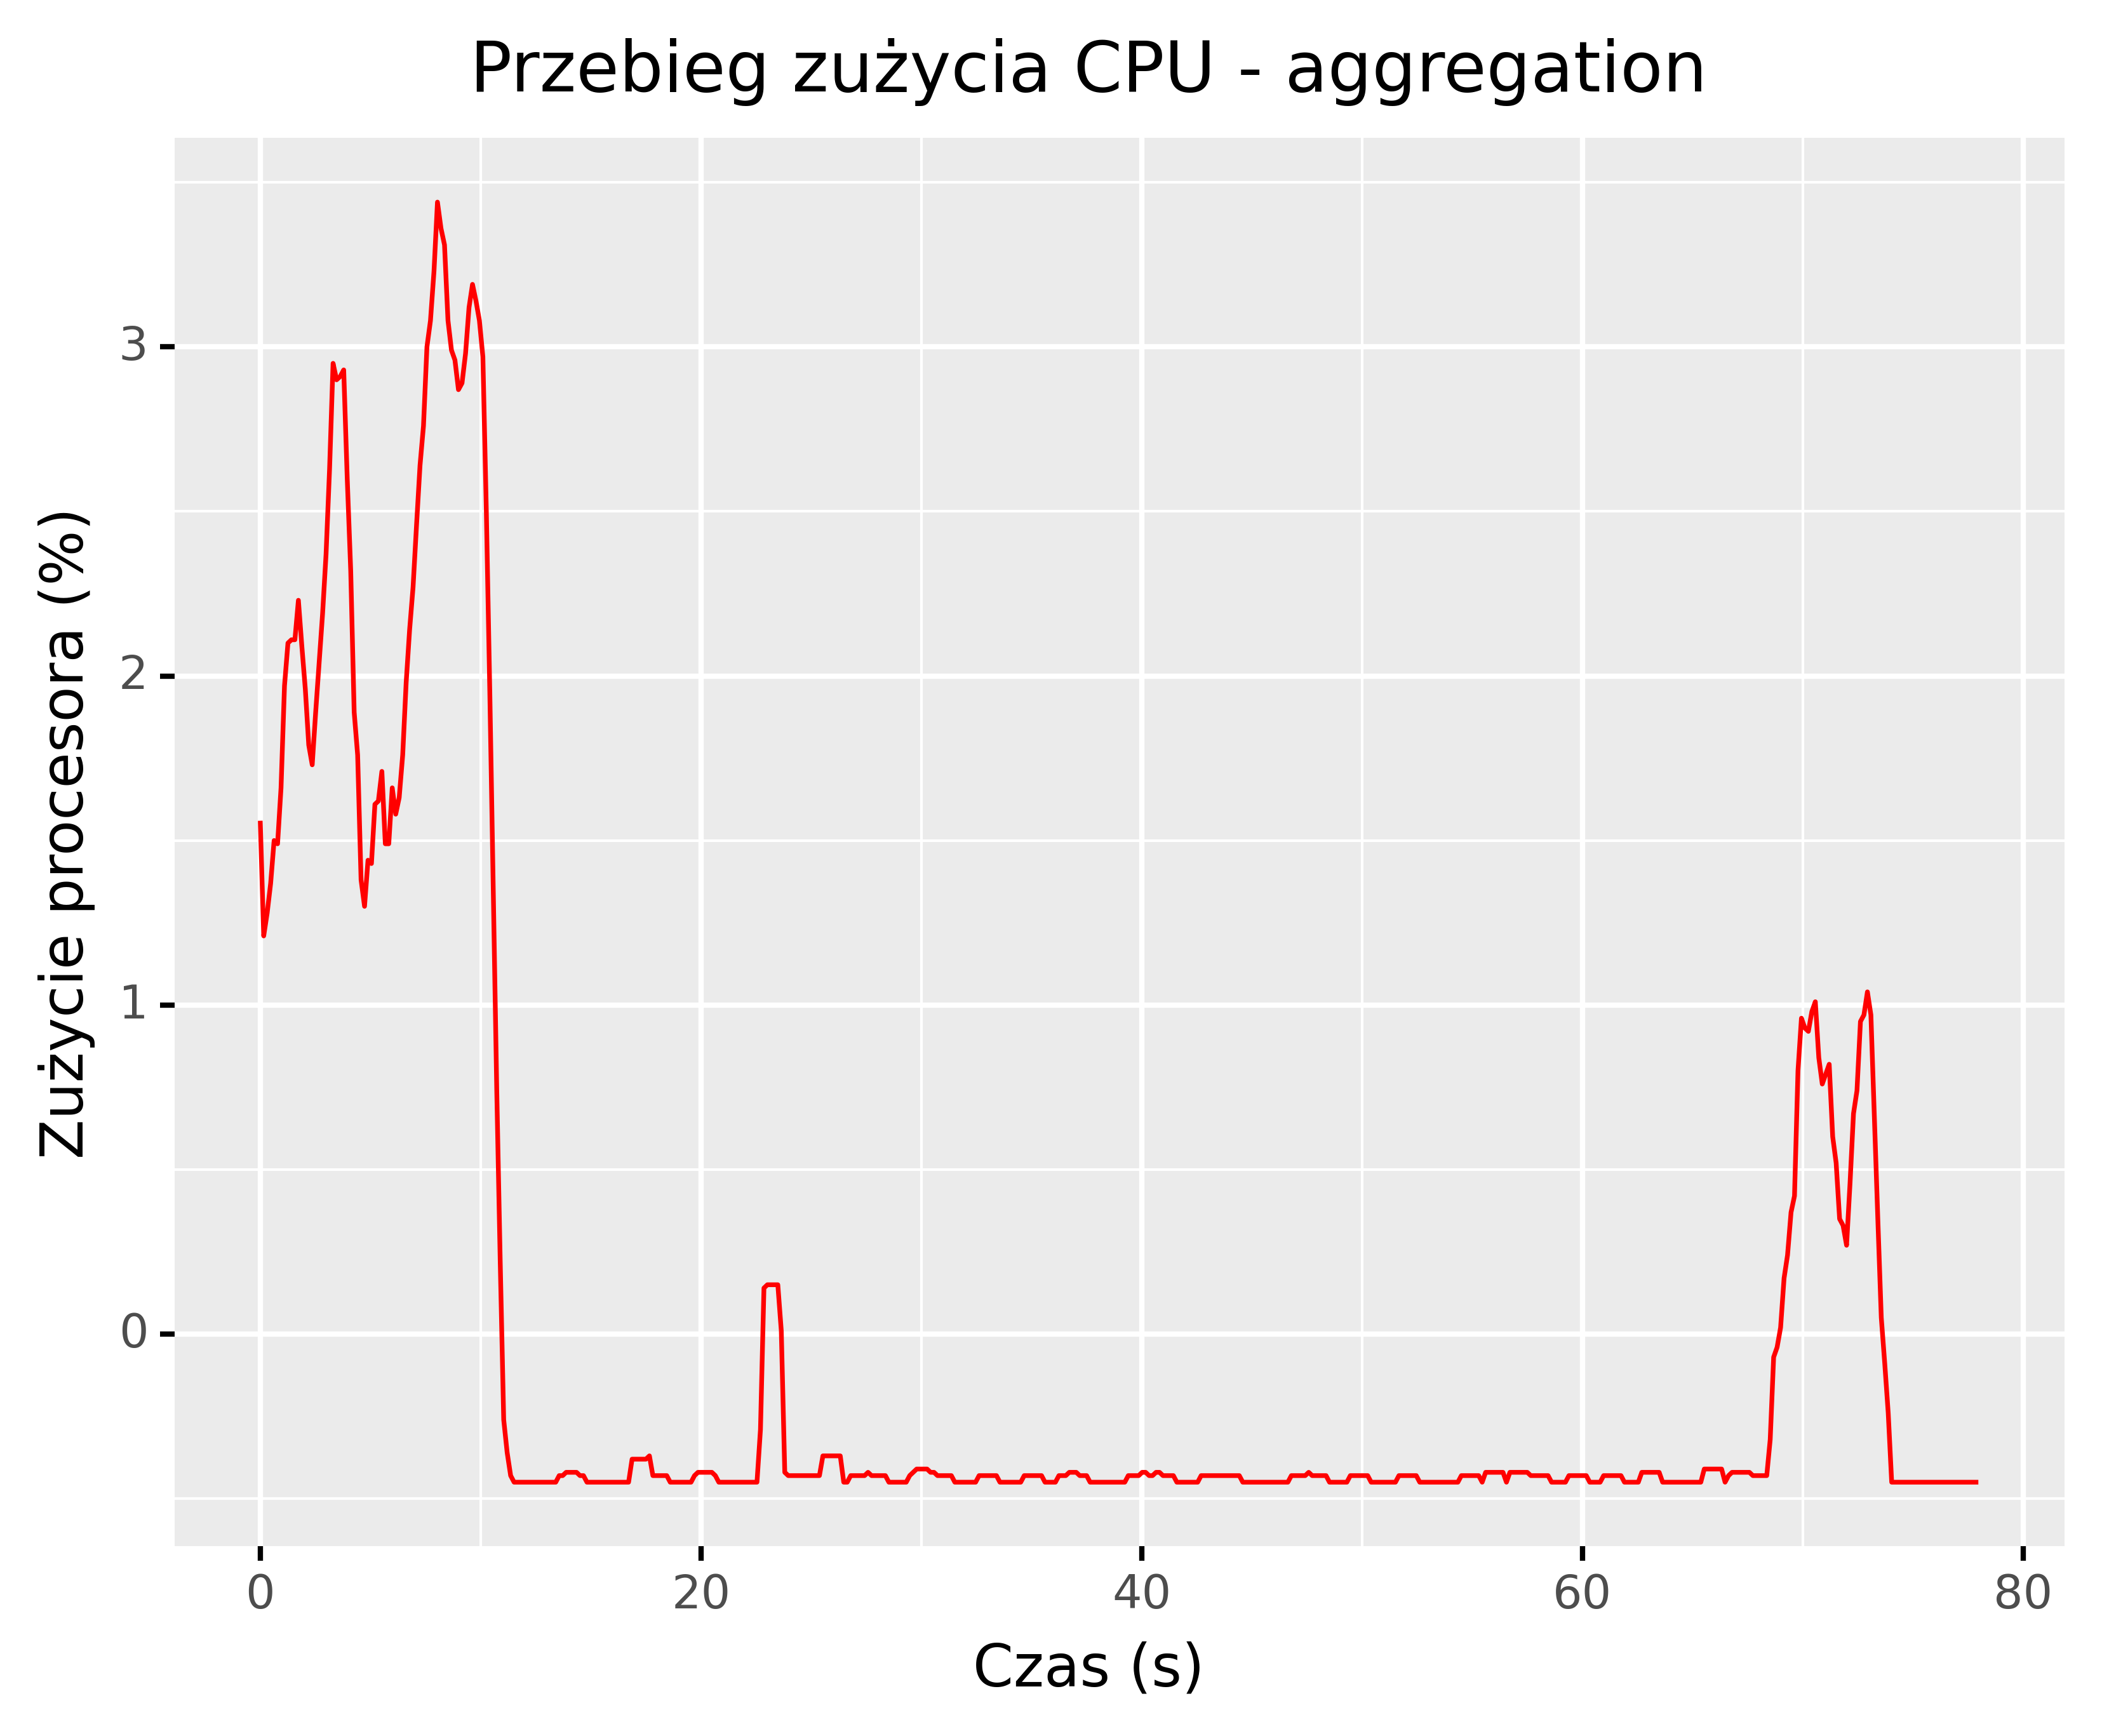
\includegraphics[width=0.5\textwidth]{figures/04-opis-danych/aggregation_smooth_standardised_cpu_snapshot_1.png}\label{aggregation_standardised:cpu}}
  \hfill
  \subfloat[RAM]{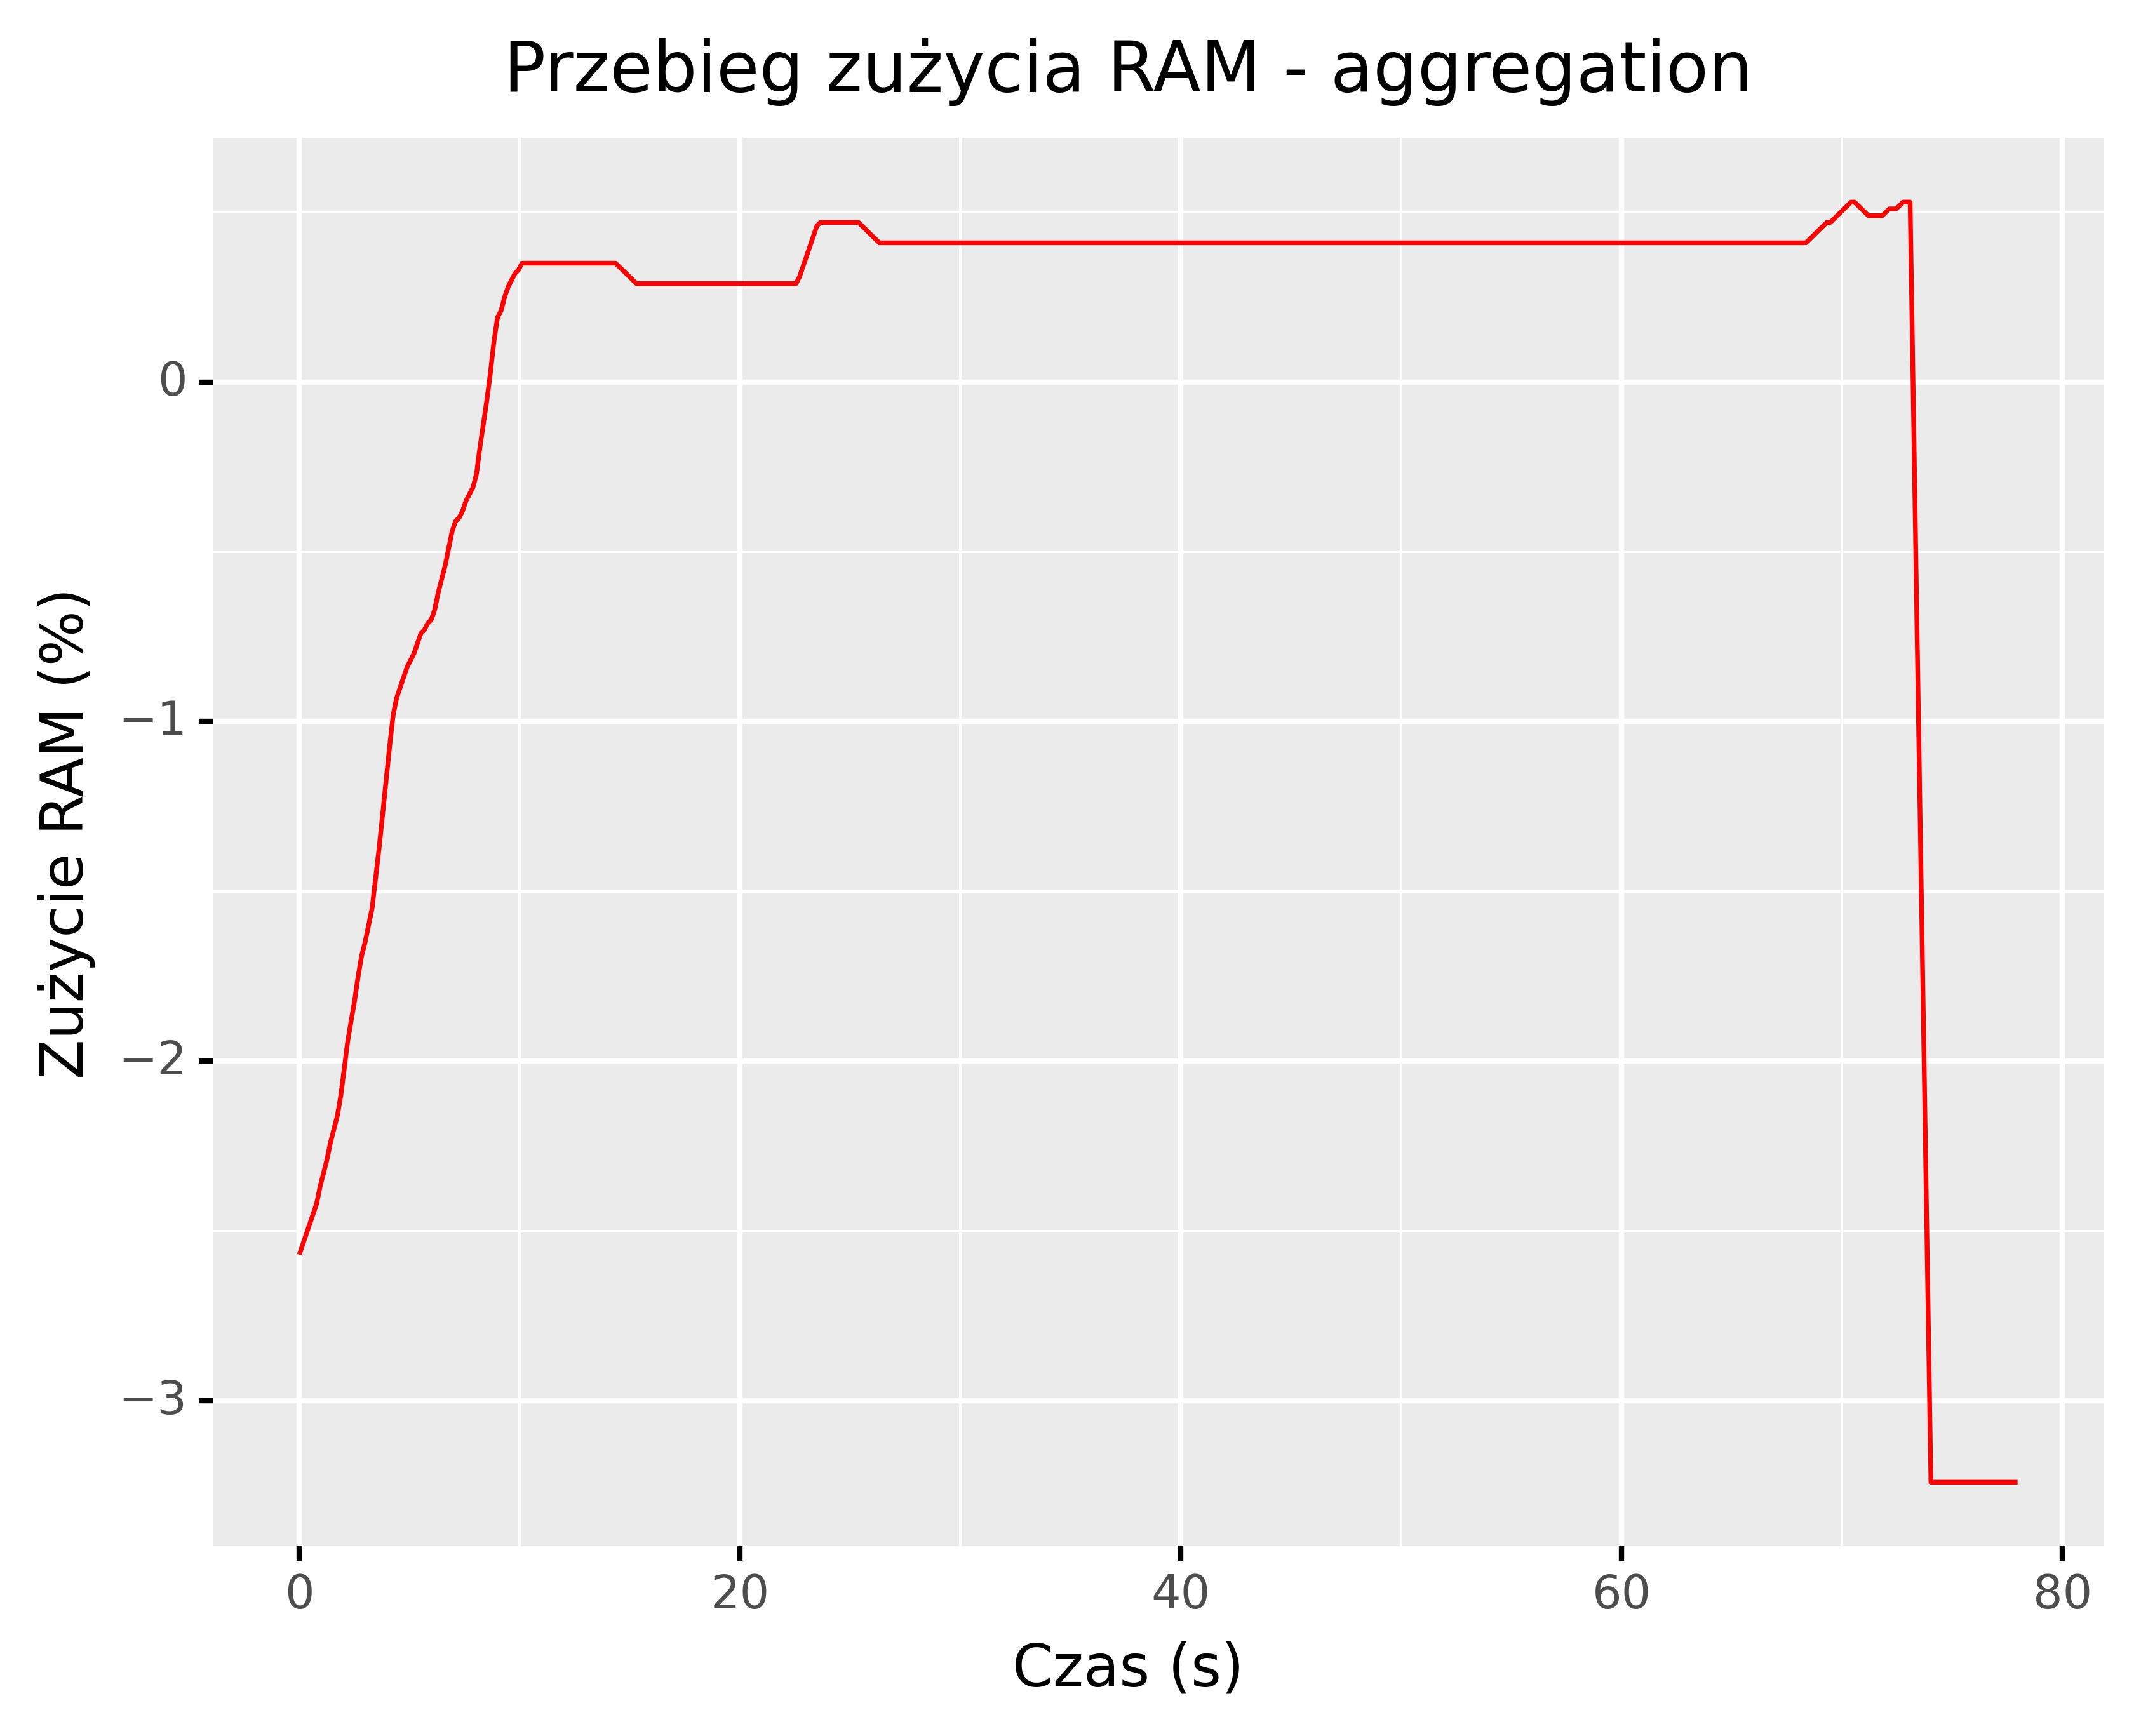
\includegraphics[width=0.5\textwidth]{figures/04-opis-danych/aggregation_smooth_standardised_ram_snapshot_1.png}\label{aggregation_standardised:ram}}
  \caption{Przykładowy ustandaryzowany wykres zużycia zasobów dla agregacji (snapshot = 1))}
  \label{aggregation_standardised}
\end{figure}

Na wykresach \ref{aggregation_standardised} widać że po wykonaniu standaryzacji kształt wykresów się nie zmienił (porównując z \ref{aggregation_smooth_6}), jednak amplitudy zmalały. W ten sposób przygotowane dane zostaną wykorzystane w eksperymentach, sprawdzając ich skuteczność przed i po standaryzacji.

\section{Charakterystyka danych wejściowych}
\begin{itemize}
    \item usunięcie identyfikatorów procesów
    \item zgrupowanie względem znacznika czasowego i zsumowanie
    \item analiza danych od około 50 próbki
\end{itemize}
\section{Cechy danych w kontekście wyboru algorytmu}
\subsection{Porównanie próbek o tych samych parametrach}
\begin{itemize}
    \item mogą się zdarzyć wartości odstające - z czym średnio radzi sobie odległość Euklidesowa
\end{itemize}
\subsection{Wpływ zmiany rozmiaru danych na uzyskany przebieg:}\begin{itemize}
    \item skalowanie amplitudy i skalowanie czasu
    \item DTW radzi sobie ze skalowaniem czasu, ale nie ze skalowaniem amplitudy. W tym wypadku prawdopodobnie lepiej zadziała Landmark Similarity
\end{itemize}

\subsection{Wpływ zmiany konfiguracji klastra (liczby węzłów roboczych) na uzyskany przebieg:}
\begin{itemize}
    \item brak większego wpływu - nie widać wpływu liczby węzłów na amplitudę lub czas
    \item skoro brak wpływu to można wykorzystać amplitudę do liczenia podobieństwa: DTW
    \item skoro brak wpływu na czas to odległość Euklidesowa również powinna być odpowiednia
    \item Sam Landmark Similarity nie wykorzystywałby informacji o amplitudzie i podobnym czasie 
\end{itemize}

\section{Wyniki eksperymentów}
Wykorzystane implementacje algorytmów:
\begin{itemize}
    \item scipy.spatial - distance.euclidean()
    \item dtw-python - distance(), normalizeDistance()
    \item dtaidistance - distance()
\end{itemize}
\subsection{dtw-python}
https://dynamictimewarping.github.io/python/
\newline
JSS Journal of Statistical Software: August 2009, Volume 31, Issue 7 \par
Computing and Visualizing Dynamic Time Warping
Alignments in R: The dtw Package
\newline Parametry \begin{itemize}
    \item {\texttt{step\_pattern} : symmetric2} - The so-called symmetric recursion printed above allows an unlimited number of elements of the query to be matched to a single element of the reference, and vice-versa
    \item {\texttt{dist\_method} : euclidean}
    \item {\texttt{keep\_internals} : true}
    \item {Funkcja normalizująca zależy od wartości step pattern, dla symmetric2 jest to N + M, gdzie N jest liczbą wartości
query sequence a M jest liczbą wartości reference, nie każdy step pattern umożliwia normalizację}
\end{itemize}

\subsection{dtaidistance}
https://dtaidistance.readthedocs.io/en/latest/usage/dtw.html



\subsection {CPU}
\begin{table}[H]
\begin{tabular}{llllll}
\hline
Funkcja:snap & Funkcja:snap &
  \begin{tabular}[c]{@{}l@{}}Euklides \\ scipy.spatial \\ distance.euclidean\end{tabular} &
  \begin{tabular}[c]{@{}l@{}}DTW \\ dtw-python \\ normalizedDistance\end{tabular} &
  \begin{tabular}[c]{@{}l@{}}DTW \\ dtw-python \\ distance\end{tabular} &
  \begin{tabular}[c]{@{}l@{}}DTW \\ dtaidistance \\distance\end{tabular} \\ \hline\hline
Aggregation:0 & Aggregation:0 & 0.0 & 0.0 & 0.0 & 0.0  \\ \hline
Aggregation:0 & Aggregation:1 & 982.23 & 3.68 & 3901.6 & 313.9  \\ \hline
Aggregation:0 & Aggregation:2 & 466.87 & 3.26 & 3646.5 & 282.45  \\ \hline
Aggregation:1 & Aggregation:2 & 984.49 & 4.04 & 4249.4 & 349.83  \\ \hline
Aggregation:0 & Filtration:1 & 1086.92 & 6.75 & 4820.7 & 450.45  \\ \hline
Aggregation:0 & Filtration:2 & 1045.09 & 7.61 & 5344.4 & 546.67 \\ \hline
Aggregation:1 & Filtration:2 & 863.54 & 6.72 & 4265.2 & 474.83  \\ \hline
\hline
\end{tabular}
\end{table}

\subsection {CPU - ustandaryzowane}
\begin{table}[H]
\begin{tabular}{llllll}
\hline
Funkcja:snap & Funkcja:snap &
  \begin{tabular}[c]{@{}l@{}}Euklides \\ scipy.spatial \\ distance.euclidean\end{tabular} &
  \begin{tabular}[c]{@{}l@{}}DTW \\ dtw-python \\ normalizedDistance\end{tabular} &
  \begin{tabular}[c]{@{}l@{}}DTW \\ dtw-python \\ distance\end{tabular} &
  \begin{tabular}[c]{@{}l@{}}DTW \\ dtaidistance \\distance\end{tabular} \\ \hline\hline
Aggregation:0 & Aggregation:0 & 0.0 & 0.0 & 0.0 & 0.0  \\ \hline
Aggregation:0 & Aggregation:1 & 11.61 & 0.06 & 65.72 & 3.93  \\ \hline
Aggregation:0 & Aggregation:2 & 5.69 & 0.04 & 48.11 & 3.63  \\ \hline
Aggregation:1 & Aggregation:2 & 11.65 & 0.07 & 76.15 & 4.34  \\ \hline
Aggregation:0 & Filtration:1 & 16.71 & 0.23 & 166.58 & 11.35  \\ \hline
Aggregation:0 & Filtration:2 & 16.94 & 0.27 & 187.24 & 10.7 \\ \hline
Aggregation:1 & Filtration:2 & 14.18 & 0.24 & 155.17 & 9.29  \\ \hline
\hline
\end{tabular}
\end{table}

\subsection {CPU - wygładzone}
\begin{table}[H]
\begin{tabular}{llllll}
\hline
Funkcja:snap & Funkcja:snap &
  \begin{tabular}[c]{@{}l@{}}Euklides \\ scipy.spatial \\ distance.euclidean\end{tabular} &
  \begin{tabular}[c]{@{}l@{}}DTW \\ dtw-python \\ normalizedDistance\end{tabular} &
  \begin{tabular}[c]{@{}l@{}}DTW \\ dtw-python \\ distance\end{tabular} &
  \begin{tabular}[c]{@{}l@{}}DTW \\ dtaidistance \\distance\end{tabular} \\ \hline\hline
Aggregation:0 & Aggregation:0 & 0.0 & 0.0 & 0.0 & 0.0  \\ \hline
Aggregation:0 & Aggregation:1 & 585.91 & 0.98 & 1039.23 & 82.9  \\ \hline
Aggregation:0 & Aggregation:2 & 183.22 & 0.84 & 936.97 & 53.32  \\ \hline
Aggregation:1 & Aggregation:2 & 558.51 & 1.04 & 1094.13 & 81.05  \\ \hline
Aggregation:0 & Filtration:1 & 743.74 & 5.59 & 3987.75 & 442.71  \\ \hline
Aggregation:0 & Filtration:2 & 670.66 & 5.65 & 3967.69 & 440.22 \\ \hline
Aggregation:1 & Filtration:2 & 496.35 & 5.81 & 3689.92 & 451.03  \\ \hline
\hline
\end{tabular}
\end{table}

\subsection {CPU - ustandaryzowany i wygładzony}
\begin{table}[H]
\begin{tabular}{llllll}
\hline
Funkcja:snap & Funkcja:snap &
  \begin{tabular}[c]{@{}l@{}}Euklides \\ scipy.spatial \\ distance.euclidean\end{tabular} &
  \begin{tabular}[c]{@{}l@{}}DTW \\ dtw-python \\ normalizedDistance\end{tabular} &
  \begin{tabular}[c]{@{}l@{}}DTW \\ dtw-python \\ distance\end{tabular} &
  \begin{tabular}[c]{@{}l@{}}DTW \\ dtaidistance \\distance\end{tabular} \\ \hline\hline
Aggregation:0 & Aggregation:0 & 0.0 & 0.0 & 0.0 & 0.0  \\ \hline
Aggregation:0 & Aggregation:1 & 6.93 & 0.02 & 22.54 & 1.33  \\ \hline
Aggregation:0 & Aggregation:2 & 2.18 & 0.01 & 11.07 & 0.66  \\ \hline
Aggregation:1 & Aggregation:2 & 6.54 & 0.02 & 23.77 & 1.44  \\ \hline
Aggregation:0 & Filtration:1 & 14.63 & 0.23 & 167.76 & 11.1  \\ \hline
Aggregation:0 & Filtration:2 & 14.95 & 0.27 & 188.75 & 11.57 \\ \hline
Aggregation:1 & Filtration:2 & 12.48 & 0.24 & 152.98 & 9.68  \\ \hline
\hline
\end{tabular}
\end{table}

\subsection {RAM}
\begin{table}[H]
\begin{tabular}{llllll}
\hline
Funkcja:snap & Funkcja:snap &
  \begin{tabular}[c]{@{}l@{}}Euklides \\ scipy.spatial \\ distance.euclidean\end{tabular} &
  \begin{tabular}[c]{@{}l@{}}DTW \\ dtw-python \\ normalizedDistance\end{tabular} &
  \begin{tabular}[c]{@{}l@{}}DTW \\ dtw-python \\ distance\end{tabular} &
  \begin{tabular}[c]{@{}l@{}}DTW \\ dtaidistance \\distance\end{tabular} \\ \hline\hline
Aggregation:0 & Aggregation:0 & 0.0 & 0.0 & 0.0 & 0.0  \\ \hline
Aggregation:0 & Aggregation:1 & 34.88 & 0.04 & 38.9 & 2.01  \\ \hline
Aggregation:0 & Aggregation:2 & 4.54 & 0.04 & 46.4 & 2.16  \\ \hline
Aggregation:1 & Aggregation:2 & 33.51 & 0.0 & 3.7 & 0.63  \\ \hline
Aggregation:0 & Filtration:1 & 29.34 & 0.13 & 92.3 & 6.93  \\ \hline
Aggregation:0 & Filtration:2 & 29.74 & 0.15 & 102.2 & 7.34 \\ \hline
Aggregation:1 & Filtration:2 & 27.61 & 0.23 & 145.0 & 8.04  \\ \hline
\hline
\end{tabular}
\end{table}

\subsection {RAM - ustandaryzowany}
\begin{table}[H]
\begin{tabular}{llllll}
\hline
Funkcja:snap & Funkcja:snap &
  \begin{tabular}[c]{@{}l@{}}Euklides \\ scipy.spatial \\ distance.euclidean\end{tabular} &
  \begin{tabular}[c]{@{}l@{}}DTW \\ dtw-python \\ normalizedDistance\end{tabular} &
  \begin{tabular}[c]{@{}l@{}}DTW \\ dtw-python \\ distance\end{tabular} &
  \begin{tabular}[c]{@{}l@{}}DTW \\ dtaidistance \\distance\end{tabular} \\ \hline\hline
Aggregation:0 & Aggregation:0 & 0.0 & 0.0 & 0.0 & 0.0  \\ \hline
Aggregation:0 & Aggregation:1 & 20.32 & 0.04 & 47.31 & 2.06  \\ \hline
Aggregation:0 & Aggregation:2 & 1.03 & 0.02 & 17.57 & 0.76  \\ \hline
Aggregation:1 & Aggregation:2 & 20.27 & 0.04 & 44.26 & 1.57  \\ \hline
Aggregation:0 & Filtration:1 & 15.66 & 0.25 & 177.08 & 11.89  \\ \hline
Aggregation:0 & Filtration:2 & 15.67 & 0.27 & 188.27 & 13.04 \\ \hline
Aggregation:1 & Filtration:2 & 13.65 & 0.26 & 167.23 & 10.09  \\ \hline
\hline
\end{tabular}
\end{table}

\subsection {RAM - wygładzony}
\begin{table}[H]
\begin{tabular}{llllll}
\hline
Funkcja:snap & Funkcja:snap &
  \begin{tabular}[c]{@{}l@{}}Euklides \\ scipy.spatial \\ distance.euclidean\end{tabular} &
  \begin{tabular}[c]{@{}l@{}}DTW \\ dtw-python \\ normalizedDistance\end{tabular} &
  \begin{tabular}[c]{@{}l@{}}DTW \\ dtw-python \\ distance\end{tabular} &
  \begin{tabular}[c]{@{}l@{}}DTW \\ dtaidistance \\distance\end{tabular} \\ \hline\hline
Aggregation:0 & Aggregation:0 & 0.0 & 0.0 & 0.0 & 0.0  \\ \hline
Aggregation:0 & Aggregation:1 & 30.45 & 0.02 & 23.69 & 1.1  \\ \hline
Aggregation:0 & Aggregation:2 & 4.44 & 0.01 & 10.37 & 0.6  \\ \hline
Aggregation:1 & Aggregation:2 & 29.11 & 0.01 & 7.39 & 0.69  \\ \hline
Aggregation:0 & Filtration:1 & 25.69 & 0.09 & 61.37 & 6.28  \\ \hline
Aggregation:0 & Filtration:2 & 26.17 & 0.09 & 62.59 & 6.7 \\ \hline
Aggregation:1 & Filtration:2 & 24.11 & 0.12 & 73.95 & 7.06  \\ \hline
\hline
\end{tabular}
\end{table}

\subsection {RAM - ustandaryzowany i wygładzony}
\begin{table}[H]
\begin{tabular}{llllll}
\hline
Funkcja:snap & Funkcja:snap &
  \begin{tabular}[c]{@{}l@{}}Euklides \\ scipy.spatial \\ distance.euclidean\end{tabular} &
  \begin{tabular}[c]{@{}l@{}}DTW \\ dtw-python \\ normalizedDistance\end{tabular} &
  \begin{tabular}[c]{@{}l@{}}DTW \\ dtw-python \\ distance\end{tabular} &
  \begin{tabular}[c]{@{}l@{}}DTW \\ dtaidistance \\distance\end{tabular} \\ \hline\hline
Aggregation:0 & Aggregation:0 & 0.0 & 0.0 & 0.0 & 0.0  \\ \hline
Aggregation:0 & Aggregation:1 & 17.71 & 0.02 & 17.02 & 1.68  \\ \hline
Aggregation:0 & Aggregation:2 & 0.93 & 0.01 & 7.64 & 0.54  \\ \hline
Aggregation:1 & Aggregation:2 & 17.65 & 0.02 & 19.04 & 1.28  \\ \hline
Aggregation:0 & Filtration:1 & 14.99 & 0.15 & 104.85 & 10.79  \\ \hline
Aggregation:0 & Filtration:2 & 15.2 & 0.16 & 109.56 & 11.77 \\ \hline
Aggregation:1 & Filtration:2 & 12.88 & 0.15 & 95.24 & 9.95  \\ \hline
\hline
\end{tabular}
\end{table}
\chapter{Budowa rozwiązania}


\chapter{Własne propozycje rozwiązań}

\chapter{Wyniki oceny eksperymentalnej}


\chapter{Uwagi końcowe}



%--------------------------------------
% Literatura
%--------------------------------------

\bibliographystyle{plain}{\raggedright\sloppy\small\bibliography{bibliografia}}

%--------------------------------------
% Dodatki
%--------------------------------------
\newpage\null\thispagestyle{empty}\newpage
\cleardoublepage\appendix%
\chapter{Repozytorium}
%--------------------------------------
% Informacja o prawach autorskich
%--------------------------------------
\newpage\null\thispagestyle{empty}\newpage

\ppcolophon

\end{document}